\documentclass[10pt]{book}
\usepackage{documento}
\usepackage{procesos}
\usepackage{verbatim} % comentarios
\title{CP2 - DA}
\subtitle{Componente 2: Documento de Análisis}
\author{Ingeniería de Software}
\date{\today}

\begin{document}

\maketitle
\thispagestyle{empty}
\tableofcontents
\chapter{Especificación de las Reglas del Negocio}
\chapter{Especificación de Reglas del Negocio}
%----------------------------------BR --------------------------------------%
\begin{BussinesRule}{BR1}{Jefe de División de Innovación Académica y Jefe de Departamento e Innovación curricular.}
    \BRitem[Tipo:] Estructural.
    \BRitem[Clase:] Habilitadora.
    \BRitem[Nivel:] Control.
    \BRitem[Descripción:] Solo pueden existir un Jefe de División de Innovación Académica y un Jefe de Departamento e Innovación curricular.
    \BRitem[Motivación:] Restringir el numero de Usuarios capaces de Gestionar Usuarios.
\end{BussinesRule}
%----------------------------------BR --------------------------------------%

\begin{BussinesRule}{BR2}{Jefes de Innovación Educativa.}
    \BRitem[Tipo:] Estructura.
    \BRitem[Clase:] Habilitadora.
    \BRitem[Nivel:] Control.
    \BRitem[Descripción:] Solo puede existir un único Jefe de Innovación Educativa por Unidad Académica.
    \BRitem[Motivación:] Tener un único responsable por Unidad Académica.
\end{BussinesRule}
%----------------------------------BR --------------------------------------%

\begin{BussinesRule}{BR3}{Gestión de Usuarios}
    \BRitem[Tipo:] Autorización.
    \BRitem[Clase:] Ejecutiva.
    \BRitem[Nivel:] Influencia.
    \BRitem[Descripción:] Solo los jefes (Jefe de División de Innovación Académica, Jefe de Departamento de Desarrollo e Innovación curricular y jefe de Innovación Educativa ) pueden registrar, consultar y cambiar  la información de los empleados que estén a su cargo, la organización para saber que usuario controla  la información de otro  será la siguiente:
    \begin{itemize}
        \item Jefe de División de Innovación Académica: Jefe de Departamento de Desarrollo e Innovación curricular, jefe de Innovación Educativa y analista de la DES.
        \item Jefe de Departamento de Desarrollo e Innovación curricular: ]efe de Innovación Educativa y analista de la DES.
        \item Jefe de Innovación Educativa: Docente y analista de su unidad académica.
    \end{itemize}
    \BRitem[Motivación:] Permitir a los Jefes tener un control sobre el acceso al sistema.
    \BRitem[Ejemplo Positivo:] El Jefe de División de Innovación Académica  actualiza el título de un analista.
    \BRitem[Ejemplo Negativo:] Un analista modifica  el nombre de otro analista.
\end{BussinesRule}
%----------------------------------BR --------------------------------------%
\begin{BussinesRule}{BR4}{Cada Usuario debe estar relacionado a una zona de trabajo.}
    \BRitem[Tipo:] Integradora.
    \BRitem[Clase:] Habilitadora.
    \BRitem[Nivel:] Control.
    \BRitem[Descripción:] La zona de trabajos de un Usuario se determinará de la siguiente manera:
    \begin{itemize}
        \item Jefe de División de Innovación Académica: DES.
        \item Jefe de Departamento de Desarrollo e Innovación curricular: DES.
        \item Jefe de Innovación Educativa: Unidad Académica.
        \item Docente: Unidad Académica de su Jefe de Innovación Educativa.
        \item Analista:  DES o Unidad Académica de su Jefe de Innovación Educativa.
    \end{itemize}
    \BRitem[Motivación:] Identificar que usuarios pertenecen a cada área y así saber que permisos tienen y a que información pueden acceder.
    \BRitem[Ejemplo Positivo:] La zona de trabajo de un Docente creado por el Jefe de Innovación Educativa de la ESCOM es la ESCOM.
    \BRitem[Ejemplo Negativo:] La zona de trabajo del Jefe de Innovación Educativa de la ESCOM es la DES.
\end{BussinesRule}
%----------------------------------BR --------------------------------------%
\begin{BussinesRule}{BR5}{Máquina de Estados de una Tarea.}
    \BRitem[Tipo:] Flujo.
    \BRitem[Clase:] Habilitadora.
    \BRitem[Nivel:] Control.
    \BRitem[Descripción:] Según el estado de la Tarea son los permisos de quien puede modificar la información relacionada con esta.
    \BRitem[Motivación:] Tener un mayor control sobre la información.
    \BRitem[Ejemplo Positivo:] La Tarea de registrar Mapa Curricular se aprobó después de que el analista y el jefe la revisaran.
    \BRitem[Ejemplo Negativo:] La Tarea de registrar Unidad de Aprendizaje se empezó a revisar antes de que terminara su registro.
\end{BussinesRule}
%----------------------------------BR --------------------------------------%
\begin{BussinesRule}{BR6}{Tareas de Registro.}
    \BRitem[Tipo:] Flujo.
    \BRitem[Clase:] Habilitadora.
    \BRitem[Nivel:] Control.
    \BRitem[Descripción:] Solo los Docentes pueden registrar Mapas Curriculares y Unidades de Aprendizaje.
    \BRitem[Motivación:] Cuestiones de jerarquía dentro de la Unidad Académica.
    \BRitem[Ejemplo Positivo:] El usuario Docente registra un Mapa Curricular o una Unidad de Aprendizaje.
    \BRitem[Ejemplo Negativo:] El usuario Analista registra un Mapa Curricular o una Unidad de Aprendizaje.
\end{BussinesRule}
%----------------------------------BR --------------------------------------%
\begin{BussinesRule}{BR7}{Revisión de Tareas.}
    \BRitem[Tipo:] Flujo.
    \BRitem[Clase:] Habilitadora.
    \BRitem[Nivel:] Control.
    \BRitem[Descripción:] Solo los analistas y los jefes  pueden revisar Mapas Curriculares o Unidades de Aprendizaje.
    \BRitem[Motivación:] Cuestiones de jerarquía dentro de la Unidad Académica.
    \BRitem[Ejemplo Positivo:] El Analista revisa un Mapa Curricular y sus respectivas Unidades de Aprendizaje.
    \BRitem[Ejemplo Negativo:] El Docente revisa un Mapa Curricular y Unidades de Aprendizaje.
\end{BussinesRule}
%----------------------------------BR --------------------------------------%
\begin{BussinesRule}{BR8}{Aprobación de Tareas.}
    \BRitem[Tipo:] Flujo.
    \BRitem[Clase:] Habilitadora.
    \BRitem[Nivel:] Control.
    \BRitem[Descripción:] Una Tarea es aprobada si al terminar de revisar no contiene comentarios.
    \BRitem[Motivación:] Poder saber cuando una tarea a finalizado.
    \BRitem[Ejemplo Positivo:] El Jefe de Innovación Educativa no agrego comentarios por lo que se aprueba.
    \BRitem[Ejemplo Negativo:] El Jefe de Innovación Educativa agrega comentario y aun así se aprueba el documento.
\end{BussinesRule}
%----------------------------------BR --------------------------------------%
\begin{BussinesRule}{BR9}{Aprobación de Tareas Seccionada.}
    \BRitem[Tipo:] Condición.
    \BRitem[Clase:] Habilitadora.
    \BRitem[Nivel:] Control.
    \BRitem[Descripción:]
    \BRitem[Sentencia:] Una tarea puede ser aprobada parcialmente y las secciones aprobadas no pueden ser modificadas.
    \BRitem[Motivación:] Evitar modificaciones en una sección ya aprobada.
    \BRitem[Ejemplo Positivo:] Una sección ya ha sido aprobada y no se hacen modificaciones.
    \BRitem[Ejemplo Negativo:] Una sección es aprobada y fue modificada.
\end{BussinesRule}
%----------------------------------BR --------------------------------------%
\begin{BussinesRule}{BR10}{Rechazo de Tareas.}
    \BRitem[Tipo:] Flujo.
    \BRitem[Clase:] Habilitadora.
    \BRitem[Nivel:] Control.
    \BRitem[Descripción:] Una Tarea es rechazada si al terminar de revisar contiene comentarios.
    \BRitem[Motivación:] Poder saber cuando una tarea debe volver al estado de Registro.
    \BRitem[Ejemplo Positivo:] El Jefe de Innovación Educativa agrego comentarios por lo que se rechaza.
    \BRitem[Ejemplo Negativo:] Ni el Jefe de Innovación Educativa ni el Analista agregaron comentarios y aun así se aprobó.
\end{BussinesRule}
%----------------------------------BR --------------------------------------%
\begin{BussinesRule}{BR11}{Asignar tareas.}
    \BRitem[Tipo:] Autorización.
    \BRitem[Clase:] Ejecutiva.
    \BRitem[Nivel:] Control.
    \BRitem[Descripción:] Solo los jefes pueden asignar tareas a los usuarios.
    \BRitem[Sentencia:]
    \BRitem[Motivación:] Llevar un orden y un control para la asignación de tareas.
    \BRitem[Ejemplo Positivo:] El Jefe de Departamento e Innovación curricular le asigna una tarea a un analista.
    \BRitem[Ejemplo Negativo:] El analista le asigna una tarea al Jefe de Departamento e Innovación curricular.
\end{BussinesRule}
%----------------------------------BR --------------------------------------%
\begin{BussinesRule}{BR12}{Tiempos de entregas.}
    \BRitem[Tipo:] Integridad.
    \BRitem[Clase:] Cronometrado.
    \BRitem[Nivel:] Control.
    \BRitem[Descripción:] Una tarea debe entregarse en la fecha indicada por el jefe de desarrollo e innovación curricular.
    \BRitem[Motivación:] Se tiene un control en las entregas de tareas.
    \BRitem[Ejemplo Positivo:] Una propuesta de unidad de aprendizaje puede ser revisada por un analista solo en el tiempo establecido.
    \BRitem[Ejemplo Negativo:] Una propuesta de unidad de aprendizaje puede ser revisada por un analista en cualquier momento.
\end{BussinesRule}
%----------------------------------BR --------------------------------------%
\begin{BussinesRule}{BR13}{Todos los datos solicitados son obligatorios.}
    \BRitem[Tipo:] Regla de Operación.
    \BRitem[Clase:] Habilitadora.
    \BRitem[Nivel:] Control.
    \BRitem[Descripción:] Los campos solicitados, no se pueden ser dejados en blanco.
    \BRitem[Sentencia:]
    \BRitem[Motivación: ]Que la base de datos esté siempre en un estado consistente.
    \BRitem[Ejemplo Positivo:] El usuario ingresa todos los datos solicitados y prosigue con su operación.
    \BRitem[Ejemplo Negativo: ]El usuario deja campos vacios y el sistema le permite continuar.
\end{BussinesRule}
%----------------------------------BR --------------------------------------%
\begin{BussinesRule}{BR14}{Catálogos del Sistema.}
    \BRitem[Tipo: ]Regla de inferencia de un hecho.
    \BRitem[Clase: ]Habilitadora.
    \BRitem[Nivel: ]Control.
    \BRitem[Descripción: ]Existen catálogos de:
    \begin{itemize}
        \item Modalidades\\
            Escolarizada\\
            Mixta\\
            No Escolarizada
        \item Roles\\
            Docente\\
            Analista\\
            Jefe de División de Innovación Académica\\
            Jefe de Departamento de Desarrollo e Innovación Curricular\\
            Jefe de Innovación Educativa
        \item Tareas\\
            Revisar Mapa Curricular\\
            Aprobar Mapa Curricular\\
            Registrar Unidad de Aprendizaje\\
            Revisar Unidad de Aprendizaje\\
            Aprobar Unidad de Aprendizaje
        \item Cargo\\
            Subdirector Académico\\
            Director\\
            Docente\\
            Director de Educación Superiores\\
            Directora de Educación Superiores
        \item Titulo\\
            Abogado/a\\
            Arquitecto/a\\
            Contador público titulado\\
            Doctor/a\\
            Ingeniero/a\\
            Licenciado/a\\
            Máster || Magíster\\
            Maestro || Ministro\\
            Maestra || Ministra\\
            Técnico
        \item Lugar de Trabajo\\
            Dirección de Estudios Superiores\\
            Dirección General\\
            Coordinación General de Formación e Innovación Educativa (CGFIE)\\
            Dirección de Formación en Lenguas Extranjeras\\
            Escuela Superior de Ingeniería Mecánica y Eléctrica (ESIME) Unidad Zacatenco \\
            Escuela Superior de Ingeniería Mecánica y Eléctrica (ESIME) Unidad Culhuacán \\
            Escuela Superior de Ingeniería Mecánica y Eléctrica (ESIME) Unidad Azcapotzalco \\
            Escuela Superior de Ingeniería Mecánica y Eléctrica (ESIME) Unidad Ticomán \\
            Escuela Superior de Ingeniería y Arquitectura (ESIA) Unidad Zacatenco \\
            Escuela Superior de Ingeniería y Arquitectura (ESIA) Unidad Tecamachalco \\
            Escuela Superior de Ingeniería y Arquitectura (ESIA) Unidad Ticomán \\
            Escuela Superior de Ingeniería Textil (ESIT) \\
            Escuela Superior de Ingeniería Química e Industrias Extractivas (ESIQIE) \\
            Escuela Superior de Física y Matemáticas (ESFM) \\
            Escuela Superior de Cómputo (ESCOM) \\
            Unidad Profesional Interdisciplinaria de Ingeniería y Ciencias Sociales y Administrativas ( UPIICSA) \\
            Unidad Profesional Interdisciplinaria en Ingeniería y Tecnologías Avanzadas (UPIITA) \\
            Unidad Profesional Interdisciplinaria de Biotecnología (UPIBI) \\
            Unidad Profesional Interdisciplinaria de Ingeniería, Campus Guanajuato (UPIIG) \\
            Unidad Profesional Interdisciplinaria de Ingeniería, Campus Zacatecas (UPIIZ) \\
            Escuela Nacional de Ciencias Biológicas (ENCB) \\
            Escuela Superior de Medicina (ESM) \\
            Escuela Nacional de Medicina y Homeopatía (ENMH) \\
            Escuela Superior de Enfermería y Obstetricia (ESEO) \\
            Centro Interdisciplinario de Ciencias de la Salud (CICS) Unidad Milpa Alta \\
            Centro Interdisciplinario de Ciencias de la Salud (CICS) Unidad Santo Tomás \\
            Escuela Superior de Comercio y Administración (ESCA) Unidad Santo Tomás \\
            Escuela Superior de Comercio y Administración (ESCA) Unidad Tepepan \\
            Escuela Superior de Economía (ESE) \\
            Escuela Superior de Turismo (EST) \\
            Centro de Lenguas Extranjeras
        \item Áreas de Formación\\
            Institucional\\
            Científica Básica\\
            Profesional\\
            Terminal y de Integración
    \end{itemize}
    \BRitem[Motivación: ]Mantener los datos en un estado consistente.
\end{BussinesRule}
%----------------------------------BR --------------------------------------%
\begin{BussinesRule}{BR15}{Planes de Estudios en re diseño por Programa Académico.}
    \BRitem[Tipo:] Relación.
    \BRitem[Clase:] Habilitadora.
    \BRitem[Nivel:] Control.
    \BRitem[Descripción:] Un Programa Académico puede tener unicamente un Plan de Estudios en rediseño.
    \BRitem[Motivación: ]Una Programa Académico puede tener varios Planes de Estudios activos pero solo se rediseña el mas actual pues este fue el rediseño de los anterior.
    \BRitem[Ejemplo Positivo:] Ingeniería en Sistemas Computacionales: ]Plan 2019.
    \BRitem[Ejemplo Negativo:] Licenciatura en Economía: ]Plan 2000, Plan 2009, Plan 2014, Plan 2018.
\end{BussinesRule}
%----------------------------------BR --------------------------------------%
\begin{BussinesRule}{BR16}{El correo electrónico del empleado es único.}
    \BRitem[Tipo: ]Relación.
    \BRitem[Clase: ]Habilitadora.
    \BRitem[Nivel: ]Control.
    \BRitem[Descripción:] Cada una de las cuentas de los empleados registrados en el sistema cuentan con un correo electrónico único.
    \BRitem[Motivación: ]Poder identificar a los usuarios.
    \BRitem[Ejemplo Positivo:] El Empleado Juan Perez tiene una correo electrónico juanp@ipn.mx  y el empleado Armando López Doriga tiene un correo electrónico armlop@ipn.mx.
    \BRitem[Ejemplo Negativo:] El Empleado Juan Perez tiene una correo electrónico juanp@ipn.mx  y el empleado Armando López Doriga tiene un correo electrónico juanp@ipn.mx.
\end{BussinesRule}
%----------------------------------BR --------------------------------------%
\begin{BussinesRule}{BR17} {El nombre de la Unidad de Aprendizaje es único.}
    \BRitem[Tipo: ]Relación.
    \BRitem[Clase: ]Habilitadora.
    \BRitem[Nivel: ]Control.
    \BRitem[Descripción: ]Cada  una de las Unidades de Aprendizaje dentro de un mismo Programa Académico tienen un nombre único.
    \BRitem[Motivación: ] Que no exista redundancia en la información y la base de datos este siempre en un estado consistente.
    \BRitem[Ejemplo Positivo:] En un Programa Académico  tenemos la materia Ingeniería de Software y Administración de Proyectos.
    \BRitem[Ejemplo Negativo: ]En un Programa Académico  tenemos la materia Ingeniería de Software y  Ingeniería de Software.
\end{BussinesRule}
%----------------------------------BR --------------------------------------%
\begin{BussinesRule}{BR18}{ Longitud máxima de Unidad de aprendizaje.}
    \BRitem[Tipo: ]Regla de inferencia de un hecho.
    \BRitem[Clase: ]Habilitadora.
    \BRitem[Nivel: ]Control.
    \BRitem[Descripción: ]El nombre de la Unidad de Aprendizaje tiene un tamaño máximo de 80 caracteres.
    \BRitem[Sentencia:]
    \BRitem[Motivación: ]Que la base de datos esté siempre en un estado consistente.
    \BRitem[Ejemplo Positivo:] El usuario llena los datos marcados con (*) y prosigue con su operación.
    \BRitem[Ejemplo Negativo: ]El usuario deja campos obligatorios y el sistema le permite continuar.
\end{BussinesRule}
%----------------------------------BR --------------------------------------%
\begin{BussinesRule}{BR19} {El nombre del Programa Académico es único.}
    \BRitem[Tipo: ]Relación.
    \BRitem[Clase: ]Habilitadora.
    \BRitem[Nivel: ]Control.
    \BRitem[Descripción: ]El nombre de los Programas Académicos es único dentro de la Unidad Académica.
    \BRitem[Motivación: ] Que no exista redundancia en la información y la base de datos este siempre en un estado consistente.
    \BRitem[Ejemplo Positivo:] En una Unidad Académica existen los Programas Académicos Ingeniería en Sistemas Computacionales y Ingeniería en Comunicaciones y Electrónica.
    \BRitem[Ejemplo Negativo: ]En una Unidad Académica existen los Programas Académicos Ingeniería en Sistemas Computacionales y Ingeniería en Sistemas Computacionales.
\end{BussinesRule}
%----------------------------------BR --------------------------------------%
\begin{BussinesRule}{BR20}{Las horas totales deben de estar entre 350 y 450 horas.}
    \BRitem[Tipo: ]Regla de operación.
    \BRitem[Clase: ]Habilitadora.
    \BRitem[Nivel: ]Control.
    \BRitem[Descripción: ]Un Plan de Estudios debe tener entre 350 y 450 horas.
    \BRitem[Motivación:] Distribuir las horas entre las unidades de aprendizaje.
    \BRitem[Ejemplo Positivo:] El usuario llena los dato de total de horas con 400 horas.
    \BRitem[Ejemplo Negativo: ] El usuario llena los dato de total de horas con 40000 horas.
\end{BussinesRule}
%----------------------------------BR --------------------------------------%
\begin{BussinesRule}{BR21}{Un libro tiene un ISBN único.}
    \BRitem[Tipo:] Regla de integridad referencial.
    \BRitem[Clase:] Habilitadora.
    \BRitem[Nivel:] Control.
    \BRitem[Descripción:] Cada uno de los libros registrados en el sistema cuentan con un ISBN único que los diferencia de otro libro aunque éstos coincidan en el nombre.
    \BRitem[Motivación:] Que no exista redundancia en la información y la base de datos esté siempre en un estado consistente.
    \BRitem[Ejemplo Positivo:] Un libro cuyo nombre es ``Ingeniería de Software'' conlleva un ISBN que es 978-92-95055-02-5, y existe otro libro con el mismo nombre ``Ingeniería de Software'' sin embargo su ISBN es 969-83-59550-10-3. Entonces se cumple la regla
    \BRitem[Ejemplo Negativo:] Para el planteamiento anterior no cumple la regla que el ISBN sea el mismo para ambos libros, puesto que uno es escrito por un autor, y el otro es escrito por otro autor.
\end{BussinesRule}
%----------------------------------BR --------------------------------------%
\begin{BussinesRule}{BR22}{Longitud del ISBN.}
    \BRitem[Tipo:] Regla de integridad estructural.
    \BRitem[Clase:] Habilitadora.
    \BRitem[Nivel:] Control.
    \BRitem[Descripción:] El ISBN se compone actualmente de trece dígitos agrupados en cinco elementos, mismos que deben estar separados por guiones de la siguiente manera:
    \begin{itemize}
        \item Prefijo Internacional (978)
        \item Identificador de grupo o Grupo de registro (607)
        \item Prefijo de editor o de Agente editor (0000)
        \item Identificador de título o publicación (00)
        \item Dígito de control o de comprobación (0)
    \end{itemize}
El resultado finalmente será: ] ISBN: ]978 - 607 - 0000 - 00 - 0
    \BRitem[Sentencia:]
    \BRitem[Motivación:] Apegarnos a las normas de la \emph{Secretaría de Cultura} y el \emph{Instituto Nacional del Derecho de Autor} para así evitar sanciones y/o incongruencias en el sistema.
    \BRitem[Ejemplo Positivo:]
    \BRitem[Ejemplo Negativo:]
\end{BussinesRule}
%----------------------------------BR --------------------------------------%
\begin{BussinesRule}{BR23}{Un libro con más de 3 autores es sólo citado por los primeros 3.}
    \BRitem[Tipo:] Regla de integridad estructural.
    \BRitem[Clase:] Habilitadora.
    \BRitem[Nivel:] Control.
    \BRitem[Descripción:] Se tomará en cuenta solamente los tres primeros autores que son referenciados en el libro.
    \BRitem[Motivación:] Seguir las normas de referencia de acuerdo al formato APA.
    \BRitem[Ejemplo Positivo:] Un libro cuyo número de autores es 5, se referencia a los autores de la siguiente manera:
    Apellido autor 1, iniciales del autor 1, Apellido autor 2, iniciales del autor 2 y Apellido de autor 3, iniciales del autor 3 (año de publicación)
    Ejemplo: Escartín, MªJ., Palomar, M. y Súarez, E. (1997)
    \BRitem[Ejemplo Negativo:] Un libro cuyo número de autores es 5, se referencia a los autores de la siguiente manera:
    Ejemplo: Escartín, MªJ., Palomar, M., Chavez, C., Salinas, L.A. y Súarez, E. (1997)
\end{BussinesRule}
%----------------------------------BR --------------------------------------%
\begin{BussinesRule}{BR24}{Debe existir al menos un criterio de evaluación para una Unidad de Aprendizaje.}
    \BRitem[Tipo:] Regla de integridad estructural.
    \BRitem[Clase:] Habilitadora.
    \BRitem[Nivel:] Control.
    \BRitem[Descripción:] Para cada Unidad de Aprendizaje debe existir al menos un criterio de evaluación cuyo porcentaje asociado sería de 100\%, sin embargo, puede tener tantos criterios como el docente decida.
    \BRitem[Motivación:] Que el docente que imparta dicha Unidad de Aprendizaje tenga al menos un referente para evaluar a sus alumnos.
    \BRitem[Ejemplo positivo:] La Unidad de Aprendizaje ``Ingeniería de Sofware'' tiene como único criterio de evaluación el desarrollo de un proyecto cuyo porcentaje equivale al 100\% de la calificación del alumno.
\end{BussinesRule}
%----------------------------------BR --------------------------------------%
\begin{BussinesRule}{BR25}{La suma de los porcentajes de cada evaluación debe ser igual a 100\%.}
    \BRitem[Tipo:] Regla de operación.
    \BRitem[Clase:] Habilitadora.
    \BRitem[Nivel:] Control.
    \BRitem[Descripción:] La suma total de los porcentajes de cada evaluación registrada por el docente, debe ser exactamente igual al 100\%.
    \BRitem[Motivación:] Que exista coherencia al momento de evaluar y que el alumno pueda identificar de dónde proviene su calificación.
    \BRitem[Ejemplo positivo:] Las evaluaciones registradas para la Unidad de Aprendizaje ``Ingeniería de Software'' son:
        \begin{itemize}
            \item 20\% Examen oral.
            \item 20\% Tareas.
            \item 60\% Proyecto final.
        \end{itemize}
        En total, los porcentajes suman el 100\% de la calificación del alumno.
\end{BussinesRule}
%----------------------------------BR --------------------------------------%
\begin{BussinesRule}{BR26}{Vigencia de una Unidad de Aprendizaje}
    \BRitem[Tipo:] Regla de integridad referencial.
    \BRitem[Clase:] Cronometrada.
    \BRitem[Nivel:] Control.
    \BRitem[Descripción:] La vigencia de una Unidad de Aprendizaje comienza en el año en el que está siendo diseñada o rediseñada hasta cinco años posteriores.
    \BRitem[Motivación:] Que los a los alumnos se les impartan las Unidades de Aprendizaje más actualizadas y no estén trabajando con cosas obsoletas.
    \BRitem[Ejemplo positivo:] Para una Unidad de Aprendizaje que está siendo diseñada o rediseñada el día 13/11/2018 cumple la regla:
        \begin{itemize}
            \item 13/11/2023.
            \item 2023.
        \end{itemize}
\end{BussinesRule}
%----------------------------------BR --------------------------------------%
\begin{BussinesRule}{BR27}{ Longitud máxima de matricula.}
    \BRitem[Tipo: ]Regla de inferencia de un hecho.
    \BRitem[Clase: ]Habilitadora.
    \BRitem[Nivel: ]Control.
    \BRitem[Descripción: ]La matricula tiene un tamaño máximo de 10 caracteres y es la matricula que tiene cada trabajador del IPN.
    \BRitem[Sentencia:]
    \BRitem[Motivación: ]Que la base de datos esté siempre en un estado consistente.
    \BRitem[Ejemplo Positivo:] . 2014171285
    \BRitem[Ejemplo Negativo: ]. 20111111111
\end{BussinesRule}
%----------------------------------BR --------------------------------------%
\begin{BussinesRule}{BR28}{ Longitud máxima de contraseña.}
    \BRitem[Tipo: ]Regla de inferencia de un hecho.
    \BRitem[Clase: ]Habilitadora.
    \BRitem[Nivel: ]Control.
    \BRitem[Descripción: ]La contraseña tiene un tamaño máximo de 6 caracteres y no debe llevar acentos.
    \BRitem[Sentencia:]
    \BRitem[Motivación: ]Que la base de datos esté siempre en un estado consistente.
    \BRitem[Ejemplo Positivo:] . abc123
    \BRitem[Ejemplo Negativo: ]. abé123333
\end{BussinesRule}
%----------------------------------BR --------------------------------------%
\begin{BussinesRule}{BR29}{Debe existir al menos un criterio de evaluación para la Relación de Prácticas.}
    \BRitem[Tipo:] Regla de integridad estructural.
    \BRitem[Clase:] Habilitadora.
    \BRitem[Nivel:] Control.
    \BRitem[Descripción:] Para cada Práctica debe existir al menos un criterio de evaluación cuyo porcentaje asociado sería de 100\%, sin embargo, puede tener tantos criterios como el docente decida.
    \BRitem[Motivación:] Que cada práctica tenga al menos un referente para evaluar a sus alumnos.
    \BRitem[Ejemplo positivo:] La Práctica 1 de la Unidad de Aprendizaje ``Ingeniería de Sofware'' tiene como único criterio de evaluación el desarrollo de un proyecto cuyo porcentaje equivale al 100\% de la calificación del alumno.
\end{BussinesRule}
%----------------------------------BR --------------------------------------%
\begin{BussinesRule}{BR30}{Información personal de usuarios y/o recursos humanos}
        \BRitem[Tipo:] Regla de integridad.
    \BRitem[Clase:] Habilitadora.
    \BRitem[Nivel:] Control.
    \BRitem[Descripción:]Se debe de contar con la siguiente información para registrar un usuario y/o recurso humano:
    \begin{itemize}
        \item Nombre
        \item Primer Apellido.
        \item Segundo Apellido.

        Estos tres datos comparten la misma expresión regular:
        \verb|/^[A-Za-záéíóúüñÁÉÍÓÚÜÑ]+(((-|')[A-Za-záéíóúüñÁÉÍÓÚÜÑ]+)|.)?( [A-Za-záéíóúüñÁÉÍÓÚÜÑ]+(((-|')[A-Za-záéíóúüñÁÉÍÓÚÜÑ]+)|.)?)*/|
        \item ***Contraseña. Expresión regular: \verb|/[^áéíóúüñÁÉÍÓÚÜÑ\s]+/|

        \item Correo electrónico.
    \end{itemize}
    ***La diferencia entre un usuario del sistema y un recurso humano registrado es que el primero posee contraseña, mientras que el segundo no. Un recurso humano se convierte en un usuario cuando se le asigna una contraseña.

    \BRitem[Motivación:] Contar con la información necesaria de los usuarios y recursos humanos para el desarrollo de las actividades.
    \BRitem[Ejemplo positivo:] Información personal del usuario o recurso humano
    \begin{itemize}
        \item Nombre: Juan Manuel
        \item Primer Apellido: Perez de
        \item Segundo Apellido: los Santos
        \item ***Contraseña: juanit8banan4 (Si se trata de un usuario)
        \item Correo electrónico: juanito@gmail.com
    \end{itemize}
    \BRitem[Ejemplo negativo:] Información personal del usuario o recurso humano
    \begin{itemize}
        \item Nombre: juan Ma. Fernando
        \item Primer Apellido: Perez de los Santos
        \item Segundo Apellido: del Carmen
        \item ***Contraseña: 132:\_147\%\$ (Si se trata de un usuario)
        \item Correo electrónico: juanito\&@gmail.com-mx/
    \end{itemize}
 \end{BussinesRule}
%----------------------------------BR --------------------------------------%
\begin{BussinesRule}{BR31}{Información de Programa Académico.}
    \BRitem[Tipo:] Regla de integridad.
    \BRitem[Clase:] Habilitadora.
    \BRitem[Nivel:] Control.
    \BRitem[Descripción:]Se debe de contar con la siguiente información para registrar un Programa Académico:
    \begin{itemize}
        \item Nombre
        Este dato tiene la expresión regular:
     \verb|[\wéíóúüñÁÉÍÓÚÜÑ]+( [\wáéíóúüñÁÉÍÓÚÜÑ+])*|
    \end{itemize}
    \BRitem[Motivación:] Contar con la información necesaria para la gestión de un Programa Académico.
    \BRitem[Ejemplo positivo:] Información del Programa Académico
    \begin{itemize}
        \item Nombre: Ingeniería en Sistemas Computacionales
    \end{itemize}
    \BRitem[Ejemplo negativo:] Información del Programa Académico
    \begin{itemize}
    \item Nombre: Ingeniería\% \_en\ Sistemas\ Computacionales\
    \end{itemize}
 \end{BussinesRule}
%----------------------------------BR --------------------------------------%
 \begin{BussinesRule}{BR32}{ Longitud máxima de nombre de Programa Académico.}
    \BRitem[Tipo: ]Regla de inferencia de un hecho.
    \BRitem[Clase: ]Habilitadora.
    \BRitem[Nivel: ]Control.
    \BRitem[Descripción: ]El nombre del Programa Acádémico tiene una longitud máxima de 150 basada en el modelo de datos.
    \BRitem[Sentencia:]
    \BRitem[Motivación: ]Que la base de datos esté siempre en un estado consistente.
    \BRitem[Ejemplo Positivo:] . Ingeniería en Sistemas Computacionales
    \BRitem[Ejemplo Negativo: ]. Ingeniería en Sistemas Computacionales Ingeniería en Sistemas Computacionales Ingeniería en Sistemas Computacionales Ingeniería en Sistemas Computacionales Ingeniería en Sistemas Computacionales
\end{BussinesRule}
%----------------------------------BR --------------------------------------%
\begin{BussinesRule}{BR33}{Información del Plan de Estudio.}
	\BRitem[Tipo:] Regla de integridad.
	\BRitem[Clase:] Habilitadora.
	\BRitem[Nivel:] Control.
	\BRitem[Descripción:]Se debe de contar con la siguiente información para registrar el Plan de Estudios:
	\begin{itemize}
		\item Programa Académico. Se obtiene por medio de un select.
		\item Año. Expresión regular: \verb|\d{4}|
		\item Modalidad. Se obtiene por medio de un select.
		\item Créditos totales TEPIC. Expresión Regular: \verb|\d+(\.\d{1,2})?|
		\item Créditos totales SATCA. Expresión Regular: \verb|\d+(\.\d{1,2})?|
		\item Total Horas/Teoría. Expresión Regular: \verb|\d{3,}|
		\item Total Horas/Práctica. Expresión Regular: \verb|\d{3,}|
	\end{itemize}
	\BRitem[Motivación:] Contar con la información necesaria del Plan de Estudio para el desarrollo de las actividades.
	\BRitem[Ejemplo positivo:] Información del Plan de Estudios
	\begin{itemize}
		\item Año: 2008
		\item Créditos totales TEPIC: 450
		\item Créditos totales SATCA: 328.55
		\item Total Horas/ Teoría: 150
		\item Total Horas/ Práctica: 150
	\end{itemize}
	\BRitem[Ejemplo negativo:] Información del Plan de Estudios
	\begin{itemize}
		\item Año: 18
		\item Créditos totales TEPIC: 302.5 6
		\item Créditos totales SATCA: 1 . 5
		\item Total Horas/ Teoría: 104
		\item Total Horas/ Práctica: 568
	\end{itemize}
\end{BussinesRule}
%----------------------------------BR --------------------------------------%
\begin{BussinesRule}{BR34}{Información de Unidad de Aprendizaje.}
	\BRitem[Tipo:] Regla de integridad.
	\BRitem[Clase:] Habilitadora.
	\BRitem[Nivel:] Control.
	\BRitem[Descripción:]Se debe de contar con la siguiente información para registrar una Unidad de Aprendizaje:
	\begin{itemize}
		\item Nombre. Expresión Regular: /[A-Za-záéíóúüñÁÉÍÓÚÜÑ]+( [A-Za-záéíóúüñÁÉÍÓÚÜÑ]+)*/
		\item Créditos TEPIC. Expresión Regular: \verb|\d+(\.\d{2})?|
		\item Créditos SATCA. Expresión Regular: \verb|\d+(\.\d{2})?|
		\item Horas Teoría/Semana. Expresión Regular: \verb|\d{2}|
		\item Horas Práctica/Semana. Expresión Regular: \verb|\d{2}|
		\item Área de Formación. Se obtiene por medio de un select.
		\item Semestre. Se obtiene por medio de un select.
	\end{itemize}
	\BRitem[Motivación:] Contar con la información necesaria de la Unidad de aprendizaje para el desarrollo de las actividades.
	\BRitem[Ejemplo positivo:] Información de la Unidad de Aprendizaje
	\begin{itemize}
		\item Nombre: Ingeniería de software.
		\item Créditos TEPIC: 8
		\item Créditos SATCA. 1.6
		\item Total Horas Teoría/Semana: 3
		\item Total Horas Práctica/Semana: 2
	\end{itemize}
	\BRitem[Ejemplo negativo:] Información del Plan de Estudios
	\begin{itemize}
		\item Nombre: Ingeniera de software 23 4.
		\item Créditos TEPIC: 455 . 5
		\item Créditos SATCA. 243-ñ
		\item Total Horas Teoría/Semana: tres
		\item Total Horas Práctica/Semana: cuatro
	\end{itemize}
\end{BussinesRule}
%----------------------------------BR --------------------------------------%
\begin{BussinesRule}{BR35}{Información laboral de los usuarios y recursos humanos.}
    \BRitem[Tipo:] Regla de integridad.
    \BRitem[Clase:] Habilitadora.
    \BRitem[Nivel:] Control.
    \BRitem[Descripción:] Cada usuario y recurso humano debe tener asignado:
    \begin{itemize}
        \item Un título profesional, se tomará aquel con mayor grado profesional.
        \item Un lugar de trabajo en la institución.
        \item Uno o varios cargos dentro de su lugar de trabajo.
    \end{itemize}

    Estos datos se cargarán desde un catálogo para cada campo.
    \BRitem[Motivación:] Contar con la información laboral necesaria de los usuarios y recursos humanos para el desarrollo de las actividades.
    \BRitem[Ejemplo positivo:] Información laboral del usuario o recurso humano
    \begin{itemize}
        \item Título: Doctor
        \item Lugar de trabajo: ESCOM
        \item Cargo(s): Director, docente.
    \end{itemize}
    \BRitem[Ejemplo negativo:] Información laboral del usuario o recurso humano
    \begin{itemize}
        \item Título: Licenciado y Maestro en Ciencias
        \item Lugar de trabajo: ESCOM y CIDETEC.
        \item Cargo(s): Sin cargo.
    \end{itemize}
 \end{BussinesRule}
 %----------------------------------BR --------------------------------------%
 \begin{BussinesRule}{BR36}{Calculo de Créditos TEPIC.}
     \BRitem[Tipo:] Regla de integridad.
     \BRitem[Clase:] Habilitadora.
     \BRitem[Nivel:] Control.
     \BRitem[Descripción:]Calcular los créditos TEPIC mediante las Horas/Semana.\\
     Formula: (Horas Teoría/Semana)*2 + Horas Práctica/Semana
     \BRitem[Motivación:] Validar la congruencia de los datos.
  \end{BussinesRule}

%\begin{BussinesRule}{}{}
%   \BRitem[Tipo:]
%   \BRitem[Clase:]
%   \BRitem[Nivel:]
%   \BRitem[Descripción:]
%   \BRitem[Motivación:]
    %\BRitem[Ejemplo positivo:]
%\end{BussinesRule}
\chapter{Mensajes}
\chapter{Mensajes}
% --------- \MSGdes{MSG#}{Mensaje}{Descripcion}{Nombre imagen}

% -------- INCLUIDO POR : ABIGAIL NICOLAS
\MSGdes{MSG0}{Matrícula y/o contraseña no válidas.}{Esta es la descripción.}{}

% -------- INCLUIDO POR :
\MSGdes{MSG1}{¿Seguro que desea editar el Programa Académico?}{Esta es la descripción.}{}

% -------- INCLUIDO POR :
\MSGdes{MSG2}{¿Seguro que desea cancelar la consulta de Programas Académicos?}{Esta es la descripción.}{}

% -------- INCLUIDO POR :
\MSGdes{MSG3}{¿Seguro que desea registrar un Programa Académico?}{Esta es la descripción.}{}

% -------- INCLUIDO POR : ARTURO, CINTHYA, NAIBI
\MSGdes{MSG4}{Los campos marcados con (*) son obligatorios.}{Esta es la descripción.}{}

% -------- INCLUIDO POR : ARTURO, NAIBI, CINTHYA
\MSGdes{MSG5}{Registro finalizado exitosamente.}{Esta es la descripción.}{}

% -------- INCLUIDO POR : ARTURO, NAIBI
\MSGdes{MSG6}{¿Seguro que desea cancelar el registro?}{Esta es la descripción.}{}

% -------- INCLUIDO POR : ARTURO, NAIBI
\MSGdes{MSG7}{Los catálogos necesarios no se han cargado, favor de intentarlo más tarde.}{Esta es la descripción.}{}

% -------- INCLUIDO POR : ARTURO, NAIBI
\MSGdes{MSG8}{El libro con el ISBN "Número de ISBN" ya existe.}{Esta es la descripción.}{}

% -------- INCLUIDO POR : ARTURO, NAIBI
\MSGdes{MSG9}{Por el momento no se puede realizar el registro.}{Esta es la descripción.}{}

% -------- INCLUIDO POR : CINTHYA
\MSGdes{MSG10}{Error: Primero debe seleccionar el punto en donde se agregará el comentario.}{Esta es la descripción.}{}

% -------- INCLUIDO POR : CINTHYA
\MSGdes{MSG11}{Error: Debe agregar un texto al nuevo comentario.}{Esta es la descripción.}{}

% -------- INCLUIDO POR : CINTHYA
\MSGdes{MSG12}{Ingrese su comentario en el nuevo campo de la bitácora.}{Esta es la descripción.}{}

% -------- INCLUIDO POR : CINTHYA
\MSGdes{MSG13}{Revisión de paquete finalizada. Paquete enviado.}{Esta es la descripción.}{}

% -------- INCLUIDO POR : CINTHYA
\MSGdes{MSG14}{Error al finalizar paquete.}{Esta es la descripción.}{}

% -------- INCLUIDO POR : CINTHYA
\MSGdes{MSG15}{¿Está seguro que desea cancelar la revisión? Se perderán las anotaciones que no hayas guardado anteriormente.}{Esta es la descripción.}{}

% -------- INCLUIDO POR : CINTHYA
\MSGdes{MSG16}{¿Está seguro de finalizar la revisión?}{Esta es la descripción.}{}

% -------- INCLUIDO POR : CINTHYA
\MSGdes{MSG17}{Sección Aprobada.}{Esta es la descripción.}{}

% -------- INCLUIDO POR : CINTHYA
\MSGdes{MSG18}{Revisión de Sección Finalizada.}{Esta es la descripción.}{}

% -------- INCLUIDO POR : CINTHYA
\MSGdes{MSG19}{Anotaciones en sección guardadas correctamente.}{Esta es la descripción.}{}

% -------- INCLUIDO POR : CINTHYA
\MSGdes{MSG20}{Los campos no fueron contestados correctamente.}{Esta es la descripción.}{}

% -------- INCLUIDO POR : NAIBI (CU1 )
\MSGdes{MSG21}{No hay usuarios registrados con ese cargo.}{Esta es la descripción.}{}

% -------- INCLUIDO POR : NAIBI ( CU1 )
\MSGdes{MSG22}{¿Seguro de eliminar al empleado ''Nombre'' con matrícula: ''Matrícula'' del sistema?}{Esta es la descripción.}{}

% -------- INCLUIDO POR : NAIBI
\MSGdes{MSG23}{Los porcentajes de evaluación no cumplen con el porcentaje total.}{}

% -------- INCLUIDO POR : ENRIQUE, ABI
\MSGdes{MSG24}{Por el momento la página solicitada no esta disponible.}{Esta es la descripción.}{}

% -------- INCLUIDO POR : ENRIQUE, ABI
\MSGdes{MSG25}{Servicios no disponibles por el momento.}{Esta es la descripción.}{}

% -------- INCLUIDO POR : ENRIQUE, ABI
\MSGdes{MSG26}{La matrícula ingresada no se encuentra registrada en el sistema.}{Esta es la descripción.}{}

% -------- INCLUIDO POR : ENRIQUE, RAFA
\MSGdes{MSG27}{Empleado modificado.}{Esta es la descripción.}{}

% -------- INCLUIDO POR : NAIBI
\MSGdes{MSG28}{El autor: "Nombre Primer Apellido Segundo Apellido" ya existe.}{Esta es la descripción.}{}

% -------- INCLUIDO POR : Arturo
\MSGdes{MSG29}{¿Está seguro que desea cancelar? Se perderán todos los avances sin guardar.}{Esta es la descripción.}{}

% -------- INCLUIDO POR : Arturo
\MSGdes{MSG30}{¿Está seguro que desea finalizar? Ya no podrá realizar modificaciones.}{Esta es la descripción.}{}

% -------- INCLUIDO POR : Arturo
\MSGdes{MSG31}{Los cambios se guardaron exitosamente.}{Esta es la descripción.}{}

% -------- INCLUIDO POR : Arturo
\MSGdes{MSG32}{Todos los campos son obligatorios.}{Esta es la descripción.}{}

% -------- INCLUIDO POR : Arturo
\MSGdes{MSG33}{El Recurso Humano con la Matrícula de Empleado [Número de Matrícula de Empleado] ya existe.}{Esta es la descripción.}{}

% -------- INCLUIDO POR : Arturo
\MSGdes{MSG34}{¿Está seguro que desea Eliminar al Recurso Humano con Matricula [no.matricula]?}{Esta es la descripción.}{}
%----------- REQUERIMIENTOS --------
%\chapter{Requerimientos}
%% -------------- TABLA PARA REQUERIMIENTOS FUNCIONALES ---------------- %
% Nomenclatura para la prioridad:
%	MA - Muy Alta
%	A - Alta
%	M - Media
%	B - Baja
%	MB - Muy Baja

\begin{table}[htbp!]
    \begin{requerimientos}

        \FRitem{RM1}{Gestionar Unidad de Aprendizaje}{El sistema debe permitirle al usuario Docente gestionar de las Unidades de Aprendizaje que contiene el Mapa Curricular.}{A}{Origen}
        \label{RM1}

        \FRitem{RM2}{Gestionar Usuarios de la Unidad Académica}{El sistema debe permitirle al Jefe de Innovación Educativa de  la gestión de los usuarios integrantes de la Unidad Académica (Analista y Docente).}{A}{Origen}
        \label{RM2}

        \FRitem{RM3}{Finalizar Mapa Curricular}{El sistema debe permitirle al usuario Docente finalizar el registro de las Unidades de Aprendizaje que contiene el Mapa  Curricular.}{A}{Origen}
        \label{RM3}

        \FRitem{RM4}{Guardar Mapa Curricular}{El sistema debe permitirle al usuario Docente guardar las Unidades de Aprendizaje que contiene el Mapa Curricular .}{M}{Origen}
        \label{RM4}

        \FRitem{RM5}{Consultar Mapa Curricular }{El sistema debe permitirle al usuario Docente visualizar la totalidad de los contenidos del Mapa Curricular registrados.}{M}{Origen}
        \label{RM5}

        \FRitem{RM6}{Validar congruencia en el Mapa Curricular}{ El Sistema validará la congruencia de los datos registrados.}{M}{Origen}
        \label{RM6}

        \FRitem{RM7}{Revisar Mapa Curricular}{el Sistema debe permitirle al Usuario Analista revisar el Mapa Curricular una vez que el registro haya finalizado.}{M}{Origen}
        \label{RM7}
        
        \FRitem{RM7}{Aprobar Mapa Curricular}{el Sistema debe permitirle al Usuario Jefe  de Innovación Educativa aprobar el Mapa Curricular una vez que el registro haya finalizado.}{M}{Origen}
        \label{RM8}

        \FRitem{RM8}{Enviar Comentarios}{ El Sistema debe permitirle a los Usuarios del Departamento de Innovación Educativa enviar comentarios de corrección sobre el Mapa Curricular una vez que el registro haya finalizado.}{M}{Origen}
        \label{RM9}

        \FRitem{RM9}{Visualizar Comentarios}{ El Sistema debe permitirle al Usuario Docente visualizar comentarios hechos al Mapa Curricular, tanto por el Departamento de Innovación Educativa como por la DES.}{M}{Origen}
        \label{RM10}
    \end{requerimientos}
    \caption{Requerimientos funcionales del sistema para el subproceso de elaboración del Mapa Curricular}
    \label{tbl:RFUA}
\end{table}

\begin{figure}[htbp]
    \begin{center}
        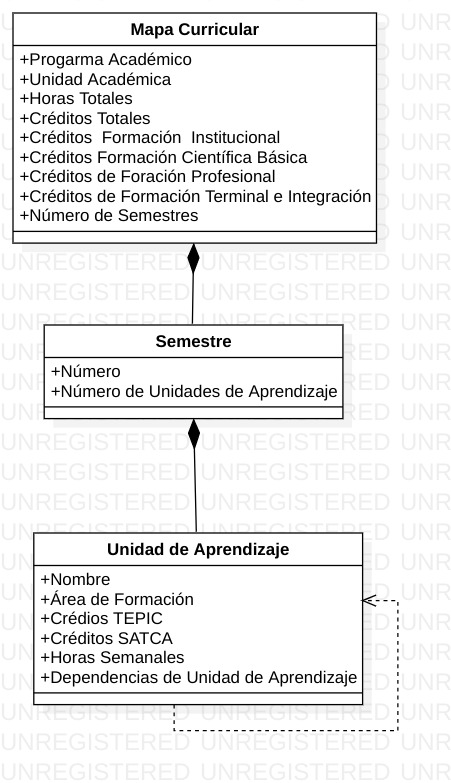
\includegraphics[width=.50\textwidth]{C2-DR/SP4/Image/ModeloDeDatosMC}
        \label{MD-SP4}
        \caption{Modelo de Datos Subproceso para la  Carga del Mapa Curricular}
    \end{center}
\end{figure}

\begin{figure}[htbp]
	\begin{center}
		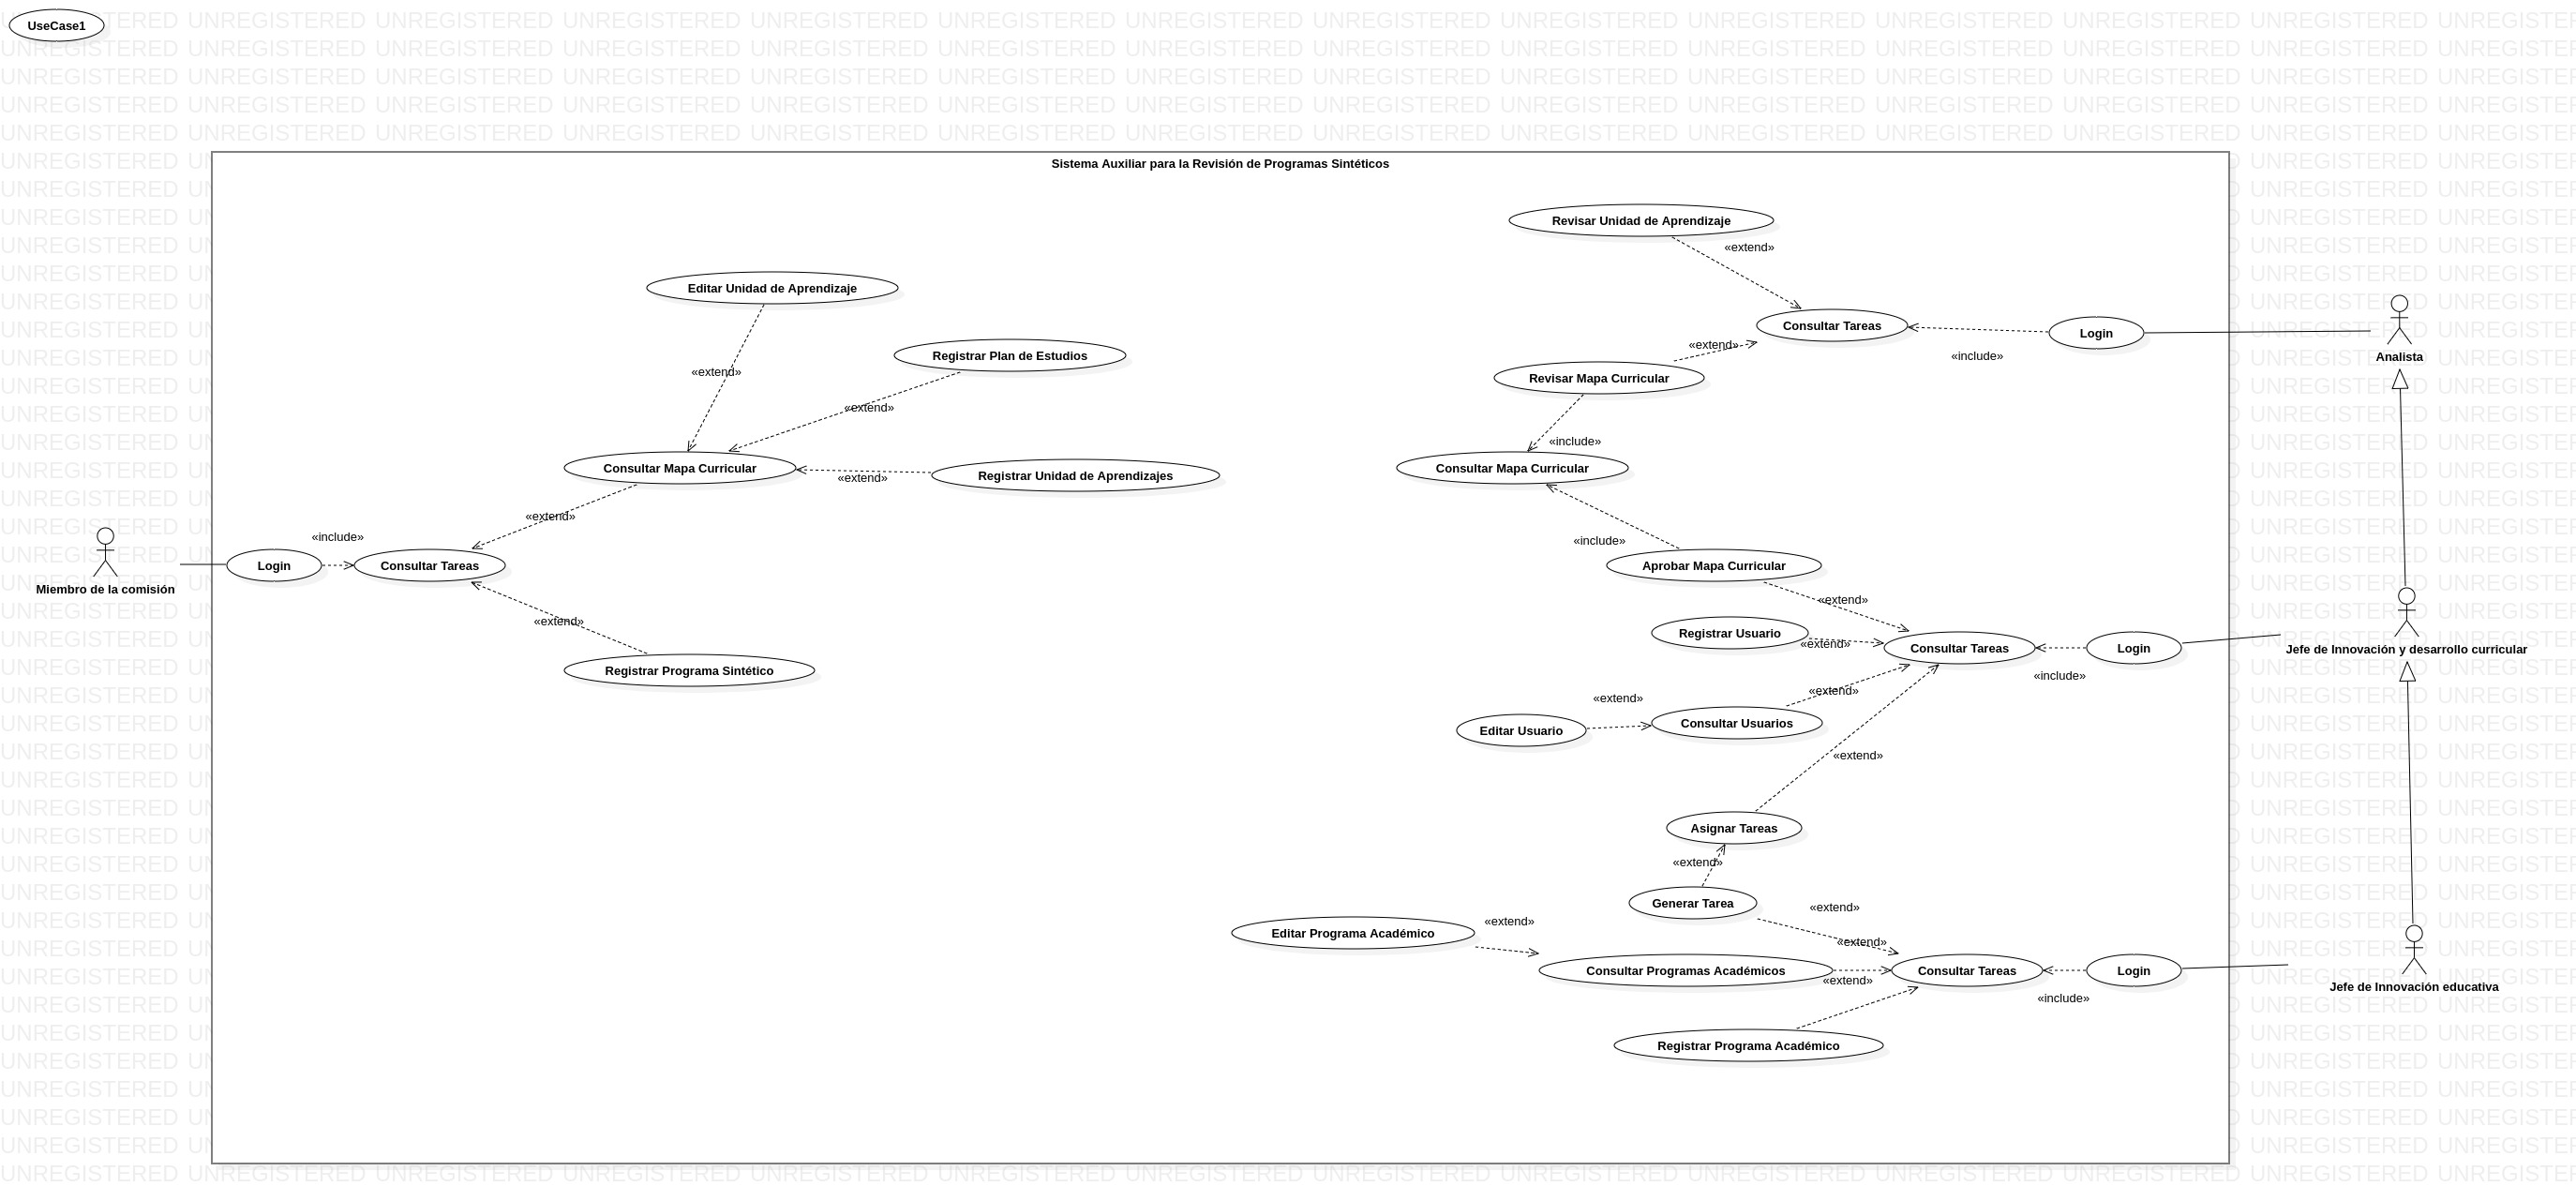
\includegraphics[width=.95\textwidth]{C2-DR/SP4/Image/CasosDeUso}
		\caption{Casos de Uso Subproceso para la  Carga del Mapa Curricular}
		\label{CU-SP4}
	\end{center}
\end{figure}

\begin{center}
	\begin{tabular}{|c|c|c|c|}
		\hline
		ID & Caso de uso & Requerimientos & Encargado \\ \hline
        1 & Registrar Mapa Curricular & \hyperref[RM1]{RM1} & Josué \\ \hline
        2 & Guardar Mapa Curricular & \hyperref[RM4]{RM4} & Andrés \\ \hline
        3 & Consultar Mapa Curricular & \hyperref[RM5]{RM5} & Arturo \\ \hline
		4 & Editar Información General & \hyperref[RM6]{RM6} & Josué \\ \hline
        5 & Finalizar Mapa Curricular & \hyperref[RM3]{RM3} & Josué \\ \hline
        6 & Aprobar Mapa Curricular & \hyperref[RM11]{RM11} & Andrés \\ \hline
        7 & Registrar Unidades de Aprendizaje & \hyperref[RM2]{RM2} & Arturo \\ \hline
        8 & Editar Unidades de Aprendizaje & \hyperref[RM8]{RM8} & Andrés \\ \hline
        9 & Eliminar Unidades de Aprendizaje & \hyperref[RM7]{RM7} & Arturo \\ \hline
        10 & Registrar Dependencias & \hyperref[RM9]{RM9} & Andrés \\ \hline
        11 & Editar Dependencias & \hyperref[RM9]{RM9} & Josué \\ \hline
        12 & Eliminar Dependencias & \hyperref[RM9]{RM9} & Arturo \\ \hline
        13 & Visualizar Comentarios & \hyperref[RM13]{RM13} & Josué \\ \hline
        14 & Enviar Comentarios & \hyperref[RM12]{RM12} & Andrés \\ \hline
    \end{tabular}
\end{center}

%% -------------- TABLA PARA REQUERIMIENTOS FUNCIONALES NAIBI---------------- % 
% Nomenclatura para la prioridad: 
%	A - Alta
%	M - Media
%	B - Baja

\begin{requerimientos}
	\FRitem{SP1-U1}{Registrar bibliografía de la UA}{El usuario registra la bibliografía de la Unidad de Aprendizaje}{A}{Usuario}
		
	\FRitem{SP1-U2}{Modificar bibliografía de la UA}{El usuario modifica la bibliografía de la Unidad de Aprendizaje}{A}{Usuario}

	\FRitem{SP1-U3}{Actualizar bibliografía de la UA}{El usuario actualiza la bibliografía de la Unidad de Aprendizaje}{A}{Usuario}

	\FRitem{SP1-U4}{Consultar bibliografía de la UA}{El usuario consulta la bibliografía de la Unidad de Aprendizaje}{A}{Usuario}

	\FRitem{SP1-U5}{Aprobar bibliografía de la UA}{El usuario aprueba la bibliografía de la Unidad de Aprendizaje}{A}{Usuario}

	\FRitem{SP1-U6}{Registrar autores de la bibliografía}{El usuario registra los autores la bibliografía}{A}{Usuario}

	\FRitem{SP1-U7}{Modificar autores de la bibliografía}{El usuario modifica los autores la bibliografía}{A}{Usuario}

	\FRitem{SP1-U8}{Actualizar autores de la bibliografía}{El usuario actualiza los autores la bibliografía}{A}{Usuario}

	\FRitem{SP1-U9}{Consultar autores de la bibliografía}{El usuario consulta los autores la bibliografía}{A}{Usuario}

	\FRitem{SP1-U10}{Registrar los tiempos de la UA}{El usuario registra los tiempos asignados de la Unidad de Aprendizaje}{A}{Usuario}
	
	\FRitem{SP1-U11}{Modificar los tiempos de la UA}{El usuario modifica los tiempos asignados de la Unidad de Aprendizaje}{A}{Usuario}
	
	\FRitem{SP1-U12}{Actualizar los tiempos de la UA}{El usuario actualiza los tiempos asignados de la Unidad de Aprendizaje}{A}{Usuario}
		
	\FRitem{SP1-U13}{Consultar los tiempos de la UA}{El usuario consulta los tiempos asignados de la Unidad de Aprendizaje}{A}{Usuario}
    
    \FRitem{SP1-U14}{Registrar la enseñanza de la UA}{El usuario registra la enseñanza de la Unidad de Aprendizaje}{A}{Usuario}
		
	\FRitem{SP1-U15}{Modificar la enseñanza de la UA}{El usuario modifica la enseñanza de la Unidad de Aprendizaje}{A}{Usuario}

	\FRitem{SP1-U16}{Actualizar la enseñanza de la UA}{El usuario actualiza la enseñanza de la Unidad de Aprendizaje}{A}{Usuario}

	\FRitem{SP1-U17}{Consultar la enseñanza de la UA}{El usuario consulta la enseñanza de la Unidad de Aprendizaje}{A}{Usuario}

	\FRitem{SP1-U18}{Registrar la evaluación de la UA}{El usuario registra la evaluación de la Unidad de Aprendizaje}{A}{Usuario}

	\FRitem{SP1-U19}{Modificar la evaluación de la UA}{El usuario modifica la evaluación de la Unidad de Aprendizaje}{A}{Usuario}

	\FRitem{SP1-U20}{Actualizar la evaluación de la UA}{El usuario actualiza la evaluación de la Unidad de Aprendizaje}{A}{Usuario}

	\FRitem{SP1-U21}{Consultar la evaluación de la UA}{El usuario consulta la evaluación de la Unidad de Aprendizaje}{A}{Usuario}
	
	\FRitem{SP1-U22}{Registrar la evaluación de la UT}{El usuario registra la evaluación de la Unidad Temática}{A}{Usuario}

	\FRitem{SP1-U23}{Modificar la evaluación de la UT}{El usuario modifica la evaluación de la Unidad Temática}{A}{Usuario}

	\FRitem{SP1-U24}{Actualizar la evaluación de la UT}{El usuario actualiza la evaluación de la Unidad Temática}{A}{Usuario}

	\FRitem{SP1-U25}{Consultar la evaluación de la UT}{El usuario consulta la evaluación de la Unidad Temática}{A}{Usuario}

	\FRitem{SP1-U26}{Registrar las UT de la UA}{El usuario registra las Unidades Temáticas de la Unidad de Aprendizaje}{A}{Usuario}

	\FRitem{SP1-U27}{Modificar las UT de la UA}{El usuario modifica las Unidades Temáticas de la Unidad de Aprendizaje}{A}{Usuario}

	\FRitem{SP1-U28}{Actualizar las UT de la UA}{El usuario actualiza las Unidades Temáticas de la Unidad de Aprendizaje}{A}{Usuario}

	\FRitem{SP1-U29}{Consultar las UT de la UA}{El usuario consulta las Unidades Temáticas de la Unidad de Aprendizaje}{A}{Usuario}

	\FRitem{SP1-U30}{Registrar los contenidos de la UA}{El usuario registra los contenidos de la Unidad Temática}{A}{Usuario}

	\FRitem{SP1-U31}{Modificar los contenidos de la UA}{El usuario modifica los contenidos de la Unidad Temática}{A}{Usuario}

	\FRitem{SP1-U32}{Actualizar los contenidos de la UA}{El usuario actualiza los contenidos de la Unidad Temática}{A}{Usuario}

	\FRitem{SP1-U33}{Consultar los contenidos de la UA}{El usuario consulta los contenidos de la Unidad Temática}{A}{Usuario}

	\FRitem{SP1-U34}{Registrar la acreditación de la UA}{El usuario registra la acreditación de la Unidad de Aprendizaje}{A}{Usuario}

	\FRitem{SP1-U35}{Modificar la acreditación de la UA}{El usuario modifica la acreditación de la Unidad de Aprendizaje}{A}{Usuario}

	\FRitem{SP1-U36}{Actualizar la acreditación de la UA}{El usuario actualiza la acreditación de la Unidad de Aprendizaje}{A}{Usuario}

	\FRitem{SP1-U37}{Consultar la acreditación de la UA}{El usuario consulta la acreditación de la Unidad de Aprendizaje}{A}{Usuario}

	\FRitem{SP1-U38}{Registrar el tipo de la UA}{El usuario registra el tipo de la Unidad de Aprendizaje}{A}{Usuario}

	\FRitem{SP1-U39}{Modificar el tipo de la UA}{El usuario modifica el tipo de la Unidad de Aprendizaje}{A}{Usuario}

	\FRitem{SP1-U40}{Actualizar el tipo de la UA}{El usuario actualiza el tipo de la Unidad de Aprendizaje}{A}{Usuario}

	\FRitem{SP1-U41}{Consultar el tipo de la UA}{El usuario consulta el tipo de la Unidad de Aprendizaje}{A}{Usuario}

	\FRitem{SP1-U42}{Registrar las prácticas de la UA}{El usuario registra las prácticas de la Unidad de Aprendizaje}{A}{Usuario}

	\FRitem{SP1-U43}{Modificar las prácticas de la UA}{El usuario modifica las prácticas de la Unidad de Aprendizaje}{A}{Usuario}

	\FRitem{SP1-U44}{Actualizar las prácticas de la UA}{El usuario actualiza las prácticas de la Unidad de Aprendizaje}{A}{Usuario}

	\FRitem{SP1-U45}{Consultar las prácticas de la UA}{El usuario consulta las prácticas de la Unidad de Aprendizaje}{A}{Usuario}

	\FRitem{SP1-U46}{Registrar la DGUA}{El usuario registra la Descripción de Unidad de Aprendizaje}{A}{Usuario}

	\FRitem{SP1-U47}{Modificar la DGUA}{El usuario modifica la Descripción de Unidad de Aprendizaje}{A}{Usuario}

	\FRitem{SP1-U48}{Actualizar la DGUA}{El usuario actualiza la Descripción de Unidad de Aprendizaje}{A}{Usuario}

	\FRitem{SP1-U49}{Consultar la DGUA}{El usuario consulta la Descripción de Unidad de Aprendizaje}{A}{Usuario}

	\FRitem{SP1-U50}{Aprobar las UA}{El usuario aprueba Unidades de Aprendizaje}{A}{Usuario}
%------------------------------------------------- EMPIEZAN LOS REQUERIMIENTOS DEL SISTEMA --------------------------------------------------%
	\FRitem{SP1-F1}{Registrar Unidades de Aprendizaje}{El sistema permite a los usuarios autorizados el registrar Unidades de Aprendizaje}{A}{RQ}
		
	\FRitem{SP1-F2}{Modificar Unidades de Aprendizaje}{El sistema permite a los usuarios autorizados el modificar Unidades de Aprendizaje}{A}{RQ}

	\FRitem{SP1-F3}{Consultar Unidades de Aprendizaje}{El sistema permite a los usuarios autorizados el consultar Unidades de Aprendizaje}{A}{RQ}

	\FRitem{SP1-F4}{Actualizar Unidades de Aprendizaje}{El sistema permite a los usuarios autorizados el actualizar Unidades de Aprendizaje}{A}{RQ}

	\FRitem{SP1-F5}{Aprobar Unidades de Aprendizaje}{El sistema permite a los usuarios autorizados el aprobar Unidades de Aprendizaje}{A}{RQ}

	\FRitem{SP1-F6}{Notificaciones de estado}{El sistema envía notificaciones del estado de la Unidad de Aprendizaje}{A}{}

	\FRitem{SP1-F7}{Generación de DGUA}{El sistema genera la Descripción General de la Unidad de Aprendizaje}{A}{x}\\ 
\caption{Identificación de requerimientos}
\label{tbl:RFUA}
\end{requerimientos}

%% -------------- TABLA PARA REQUERIMIENTOS FUNCIONALES ---------------- % 
% Nomenclatura para la prioridad: 
%	MA - Muy Alta
%	A - Alta
%	M - Media
%	B - Baja
%	MB - Muy Baja

\begin{table}[htbp!]
	\begin{requerimientos}
		\FRitem{RF1}{Visualización de propuestas}{El usuario analista y JDDIC podrán visualizar  el contenido  de la propuesta de cada unidad de aprendizaje.}{A}{Usuario}
		\FRitem{RF2}{Recibo de paquetes}{El usuario JDDIC podrá recibir los paquetes de propuestas de unidades de aprendizaje del jefe de innovación educativa de la Unidad Académica correspondiente.}{A}{Usuario}
		\FRitem{RF2-1}{Asignación de paquetes}{El usuario JDDIC podrá asignar los paquetes recibidos de la Unidad Académica correspondiente a sus analistas.}{A}{Usuario}
		\FRitem{RF3}{Envío de paquetes}{El usuario JDDIC podrá mandar los paquetes al jefe de innovación educativa de la unidad académica correspondiente.}{A}{Usuario}
		\FRitem{RF4}{Creación de comentarios}{El usuario analista y JDDIC  podrán agregar comentarios a las partes no aprobadas de la propuesta de cada unidad de aprendizaje.}{A}{Usuario}
		\FRitem{RF5}{Autorización de secciones}{El analista podrá autorizar secciones de la de propuesta de unidad de aprendizaje.}{M}{Usuario}
		\FRitem{RF5-1}{Identificador de usuarios}{A los analistas y el JDDIC se les agregará una matrícula única con las que se les identifica como autores de los comentarios en la propuesta de unidad de aprendizaje}{M}{Usuario}
		\FRitem{RF5-2}{Acceso de documentos asignados}{El usuario analista sólo podrá añadir comentarios a los documentos que le fueron asignados por el usuario JDDIC.}{M}{Usuario}
		\FRitem{RF5.3}{Bloqueo de secciones autorizadas}{El sistema impedirá agregar comentarios de las secciones del documento aprobadas anteriormente.}{B}{Origen}
		\FRitem{RF5.4}{Registro de hora de actualización}{El sistema guardará la fecha y hora de cada modificación realizada en el área de comentarios por los usuarios analista y el JDDIC en el documento de propuesta de unidad de aprendizaje.}{B}{Origen}
	\end{requerimientos}
    \caption{Requerimientos funcionales del sistema.}
    \label{tbl:}
\end{table}

%% -------------- TABLA PARA REQUERIMIENTOS FUNCIONALES ---------------- %
% Nomenclatura para la prioridad:
%	MA - Muy Alta
%	A - Alta
%	M - Media
%	B - Baja
%	MB - Muy Baja

    \begin{requerimientos}

%-----------------------------------------------------Requerimeintos de Usuario-----------------------------------------------------------

        \FRitem{SP4-U1}{Registrar Programa Académico}{El usuario Jefe de Innovación Educativa registra los datos del Programas Académicos, acorde a la entidad Programa Académico del \hyperref[MDD]{Modelo de Datos}.}{A}{Origen}
        \label{SP4-U1}

        \FRitem{SP4-U2}{Registrar Plan de Estudios}{El usuario Doncente registra los datos del Plan de estudios , acorde a la entidad Plan de Estudios del \hyperref[MDD]{Modelo de Datos}.}{A}{Origen}
        \label{SP4-U2}

        \FRitem{SP4-U3}{Registrar Unidad de Aprendizaje}{El usuario Docente registra los datos de las Unidades de Aprendizaje, de acorde a la entidad Unidad de Aprendizaje del \hyperref[MDD]{Modelo de Datos},  que contiene el Mapa Curricular.}{A}{Origen}
        \label{SP4-U3}

        \FRitem{SP4-U4}{Registrar Usuarios}{El usuario Jefe de Innovación Educativa registra a los usuarios (Analista y Docente).}{A}{Origen}
        \label{SP4-U4}

        \FRitem{SP4-U5}{Consultar Programas Académicos }{El usuario Jefe de Innovación Educativa visualiza la informacion de los Programas Académicos.}{A}{Origen}
        \label{SP4-U5}

        \FRitem{SP4-U6}{Consultar Planes de Estudios }{El usuario Jefe de Innovación Educativa visualiza la informacion de los Planes de Estudios.}{A}{Origen}
        \label{SP4-U6}

        \FRitem{SP4-U7}{Consultar Tareas}{El usuario consulta las tareas en las que esta asignado.}{A}{Origen}
        \label{SP4-U7}

        \FRitem{SP4-U8}{Consultar Mapa Curricular }{El usuario Docente visualiza la totalidad de los contenidos del Mapa Curricular registrados.}{A}{Origen}
        \label{SP4-U8}

        \FRitem{SP4-U9}{Consultar Usuarios}{El usuario  Jefe de Innovación Educativa consulta los usuarios.}{A}{Origen}
        \label{SP4-U9}

        \FRitem{SP4-U10}{Finalizar Carga Mapa Curricular}{El usuario Docente finaliza el registro de todas las Unidades de Aprendizaje que contiene el Mapa  Curricular.}{A}{Origen}
        \label{SP4-U10}

        \FRitem{SP4-U11}{Asignar tareas a los usuarios de la Unidad Académica}{El usuario Jefe de Innovación Educativa asigna tareas a los usuarios.}{A}{Origen}
        \label{SP4-U11}

        \FRitem{SP4-U12}{Generar Tareas}{El usuario Jefe de Innovación Educativa genera las tareas de registro (Mapas Curriculares y Programas Sintéticos).}{A}{Origen}
        \label{SP4-U12}

        \FRitem{SP4-U13}{Consultar Tareas}{Los usuarios visualizan las tareas a las que están asignados.}{A}{Origen}
        \label{SP4-U13}

        \FRitem{SP4-U14}{Enviar Comentarios}{ Los usuarios del Departamento de Innovación Educativa envían comentarios de corrección sobre el Mapa Curricular una vez que el registro haya finalizado.}{A}{Origen}
        \label{SP4-U14}

        \FRitem{SP4-U15}{Visualizar Comentarios}{ El Usuario Docente visualiza los comentarios hechos al Mapa Curricular, tanto por el Departamento de Innovación Educativa como por la DES.}{A}{Origen}
        \label{SP4-U15}

        \FRitem{SP4-U16}{Modificar Unidad de Aprendizaje}{El usuario Docente modifica los datos de las Unidades de Aprendizaje registradas.}{M}{Origen}
        \label{SP4-U16}

        \FRitem{SP4-U17}{Eliminar Unidad de Aprendizaje}{El usuario Docente elimina las Unidades de Aprendizaje registradas.}{M}{Origen}
        \label{SP4-U17}

        \FRitem{SP4-U18}{Guardar Avances del Mapa Curricular}{El usuario Docente guarda las Unidades de Aprendizaje que este vaya registrando.}{M}{Origen}
        \label{SP4-U18}

        \FRitem{SP4-U19}{Aprobar Mapa Curricular}{El usuario Jefe  de Innovación Educativa aprueba el Mapa Curricular una vez que el registro haya finalizado.}{M}{Origen}
        \label{SP4-U19}

        \FRitem{SP4-U20}{Revisar Mapa Curricular}{El usuario Analista revisa el Mapa Curricular una vez que el registro haya finalizado.}{B}{Origen}
        \label{SP4-U20}

        \FRitem{SP4-U21}{Modificar Programa Académico}{El usuario Jefe de Innovación Educativa modifica los datos de los Programas Académicos.}{B}{Origen}
        \label{SP4-U21}

        \FRitem{SP4-U22}{Modificar Plan de Estudios}{El usuario Jefe de Innovación Educativa modifica los datos del Plan de Estudios.}{B}{Origen}
        \label{SP4-U22}

        \FRitem{SP4-U23}{Modificar Información de Usuarios}{El usuario Jefe de Innovación Educativa modifica la información general de los usuarios.}{B}{Origen}
        \label{SP4-U23}

        \FRitem{SP4-U24}{Eliminar Usuarios}{El usuario Jefe de Innovación Educativa elimina a cualquier usuario.}{B}{Origen}
        \label{SP4-U24}

        \FRitem{SP4-U25}{Login}{El usuario ingresa a su cuenta.}{B}{Origen}
        \label{SP4-U25}

        \FRitem{SP4-F1}{Registrar Programa Académico}{El sistema debe permitir que el usuario de tipo "Jefe de Innovación Educativa" registre los datos de los Programas Académicos, acorde a la entidad Programa Académico del \hyperref[MDD]{Modelo de Datos}.}{A}{Origen}
        \label{SP4-F1}

        \FRitem{SP4-F2}{Registrar Plan de Estudios}{El sistema debe permitir que el usuario de tipo "Docente" registre los datos del Plan de estudios , acorde a la entidad Plan de Estudios del \hyperref[MDD]{Modelo de Datos}.}{A}{Origen}
        \label{SP4-F2}

        \FRitem{SP4-F3}{Registrar Unidad de Aprendizaje}{El sistema debe permitir que el usuario de tipo "Docente" registre los datos de las Unidades de Aprendizaje, acorde a la entidad Unidad de Aprendizaje del \hyperref[MDD]{Modelo de Datos}.}{A}{Origen}
        \label{SP4-F3}

        \FRitem{SP4-F4}{Registrar Usuarios}{El sistema debe permitir que el usuario de tipo "Jefe de Innovación Educativa" registre a los usuarios (Analista y Docente).}{A}{Origen}
        \label{SP4-F4}

        \FRitem{SP4-F5}{Consultar Programas Académicos }{El sistema debe permitir que el usuario de tipo "Jefe de Innovación Educativa" consulte los Programas Académicos.}{A}{Origen}
        \label{SP4-F5}

        \FRitem{SP4-F6}{Consultar Planes de Estudios }{El sistema debe permitir que el usuario de tipo "Jefe de Innovación Educativa" consulte los Planes de Estudios de los Programas Académicos.}{A}{Origen}
        \label{SP4-F6}

        \FRitem{SP4-F7}{Consultar Mapa Curricular }{El sistema debe permitir que el usuario de tipo "Docente" visualice todos los registros existentes del Mapa curricular.}{A}{Origen}
        \label{SP4-F7}

        \FRitem{SP4-F8}{Consultar Usuarios}{El sistema debe permitir que el usuario de tipo "Jefe de Innovación Educativa" consulte los usuarios.}{A}{Origen}
        \label{SP4-F8}

        \FRitem{SP4-F9}{Finalizar Tarea}{El sistema debe permitir que los usuarios indiquen cuando hayan finalizado una Tarea.}{A}{Origen}
        \label{SP4-F9}

        \FRitem{SP4-F10}{Asignar tareas a los usuarios de la Unidad Académica}{El sistema debe permitir que el usuario de tipo "Jefe de Innovación Educativa" asigne tareas a los usuarios.}{A}{Origen}
        \label{SP4-F10}

        \FRitem{SP4-F11}{Generar Tareas}{El sistema debe permitir que el usuario de tipo "Jefe de Innovación Educativa" genere las tareas de registro (Mapas Curriculares y Programas Sintéticos).}{A}{Origen}
        \label{SP4-F11}

        \FRitem{SP4-F120}{Consultar Tareas}{El sistema debe permitir que los usuarios visualicen las tareas a las que están asignados.}{A}{Origen}
        \label{SP4-F12}

        \FRitem{SP4-F13}{Validar congruencia en el Mapa Curricular}{ Si algunos de los datos ingresados se contradicen el sistema no permitirá que se guarden hasta resolver el conflicto.}{A}{Origen}
        \label{SP4-F13}

        \FRitem{SP4-F14}{Enviar Comentarios}{ El sistema debe permitir que los usuarios de tipo "Analista" y  "Jefe de Innovación Educativa" envíen comentarios de corrección sobre el Mapa Curricular una vez que el usuario de tipo "Docente" haya finalizado el registro.}{A}{Origen}
        \label{SP4-F14}

        \FRitem{SP4-F15}{Visualizar Comentarios}{ El sistema debe permitir que el usuario de tipo "Docente" visualice los comentarios hechos a las tareas que este asignado, tanto los hechos por el Departamento de Innovación Educativa como por la DES.}{A}{Origen}
        \label{SP4-F15}

        \FRitem{SP4-F16}{Modificar Unidad de Aprendizaje}{El sistema debe permitir que el usuario de tipo "Docente" modifique lod dato de las Unidades de Aprendizaje que contiene el Mapa Curricular.}{M}{Origen}
        \label{SP4-F16}

        \FRitem{SP4-F17}{Eliminar Unidad de Aprendizaje}{El sistema debe permitir que el usuario de tipo "Docente" elimine las Unidades de Aprendizaje registradas.}{M}{Origen}
        \label{SP4-F17}

        \FRitem{SP4-F18}{Guardar Avances del Mapa Curricular}{El sistema debe permitirle al usuario Docente guardar las Unidades de Aprendizaje que éste vaya registrando.}{M}{Origen}
        \label{SP4-F18}

        \FRitem{SP4-F19}{Aprobar Mapa Curricular}{El sistema debe permitir que el usuario de tipo "Jefe de Innovación Educativa" apruebe el Mapa Curricular una vez que el usuario de tipo "Analista" haya finalizada la revisión.}{M}{Origen}
        \label{SP4-F19}

        \FRitem{SP4-F20}{Revisar Mapa Curricular}{El sistema debe permitir que el usuario de tipo "Analista" revise el Mapa Curricular  una vez que el usuario de tipo "Docente" haya finalizada el registro.}{B}{Origen}
        \label{SP4-F20}

        \FRitem{SP4-F21}{Modificar Programa Académico}{El sistema debe permitir que el usuario de tipo "Jefe de Innovación Educativa" modifique los datos de los Programas Académicos.}{B}{Origen}
        \label{SP4-F21}

        \FRitem{SP4-F22}{Modificar Plan de Estudios}{El sistema debe permitir que el usuario de tipo "Jefe de Innovación Educativa" modifique los datos del Plan de Estudios.}{B}{Origen}
        \label{SP4-F22}

        \FRitem{SP4-F23}{Modificar Usuarios de la Unidad Académica}{El sistema debe permitir que el usuario de tipo "Jefe de Innovación Educativa" modifique la información general de cualquier usuario.}{B}{Origen}
        \label{SP4-F23}

        \FRitem{SP4-F24}{Eliminar Usuarios de la Unidad Académica}{El sistema debe permitir que el usuario de tipo "Jefe de Innovación Educativa" elimine a cualquier usuario.}{B}{Origen}
        \label{SP4-F24}

        \FRitem{SP4-F25}{Notificar al Usuario}{El sistema informará al usuario de los cambios de estatus de las tareas a las que está asignado.}{B}{Origen}
        \label{SP4-F25}

        \FRitem{SP4-F26}{Login}{El sistema permitira al usuario ingresar a su cuenta.}{B}{Origen}
        \label{SP4-F26} \\

    \caption{Requerimientos del subproceso de elaboración del Mapa Curricular}
    \label{tbl:SP4-R}
    \end{requerimientos}

%% -------------- TABLA PARA REQUERIMIENTOS FUNCIONALES ---------------- % 
% Nomenclatura para la prioridad: 
%	A - Alta
%	M - Media
%	B - Baja

\textbf{Nota:} Se usa :
	\begin{itemize}
		\item \textbf{JDIC:} Jefe de departamento de Innovación curricular
		\item \textbf{JDIA:} Jefe de división de innovación académica
		\item \textbf{DES:} Directora de Educación Superior
	\end{itemize}

\begin{table}[htbp!]
	\begin{requerimientos}
		
		\FRitem{VMP-01}{Registrar empleados del JDIA}{El sistema permitirá al usuario JDIA registrar usuarios JDIC.}{A}{}

		\FRitem{VMP-02}{Registrar empleados del JDIC}{El sistema permitirá al usuario JDCI registrar usuarios analistas y jefes de innovación educativa.}{A}{}

		\FRitem{VMP-03}{Consultar empleados}{El sistema permitirá al JDIA y al JDIC consultar la información y trabajo activo de los analistas y jefes de innovación educativa.}{M}{}

		\FRitem{VMP-04}{Eliminar empleados del JDIA}{El sistema permitirá al JDIA eliminar usuarios JDIC.}{B}{}

		\FRitem{VMP-05}{Eliminar empleados del JDIC}{El sistema permitirá al JDCI eliminar usuarios analistas y jefes de innovación educativa.}{B}{}

		\FRitem{VMP-06}{Consultar asignaciones del analista}{El sistema le mostrará al usuario analista las tareas  que tiene asignadas.}{A}{}

		\FRitem{VMP-07}{Consultar mapas curriculares}{El JDIA y el JDIC consultarán la lista de los mapas curriculares por nombre de la unidad académica o todos los mapas curriculares registrados.}{M}{}

		\FRitem{VMP-08}{Ver mapa curricular}{El sistema mostrará al JDIA y al JDIC la información de un mapa curricular previamente seleccionado.}{A}{}

		\FRitem{VMP-09}{Asignar analista}{El JDIC seleccionará (de la lista de usuarios analista, él incluido) el empleado (visualizando su nombre y el número de tareas que tiene asignadas) que revisará el mapa curricular previamente elegido.}{M}{}

		\FRitem{VMP-10}{Atender mapa curricular por parte del JDIC}{El sistema permitirá al JDIC analizar, en conjunto con los analistas, uno o más mapas curriculares recibidos por las unidades académicas.}{A}{}

		\FRitem{VMP-11}{Comunicar observaciones del mapa curricular a los analistas}{El sistema permitirá al JDIC contactar al analista encargado de un mapa curricular para comunicarle observaciones, correcciones, notas, etcétera, respecto a éste.}{M}{}

		\FRitem{VMP-12}{Realizar modificaciones al mapa curricular}{El sistema permitirá a la JDIC realizar correcciones y ajustes a un mapa curricular, en conjunto con su analista asignado, para llegar a un acuerdo.}{A}{}

		\FRitem{VMP-13}{Delegar tareas a los analistas}{El sistema permitirá a la JDIC delegar la tarea de revisar uno o varios mapas curriculares a los analistas.}{M}{}

		\FRitem{VMP-14}{Verificar nombre de unidades de aprendizaje en el mapa curricular}{El sistema permitirá a la JDIC y a la JDIA aprobar o rechazar el nombre que se le asignó a las unidades de aprendizaje en un mapa curricular.}{A}{}

		\FRitem{VMP-15}{Iniciar revisión del mapa curricular}{Un mapa curricular enviado por la unidad académica debe tener todos sus campos completos y llenos para que se pueda iniciar el revisado por la DES en el sistema.}{A}{}

		\FRitem{VMP-16}{Realizar notas y comentarios}{El sistema permitirá al JDIC y a los analistas redactar una o más correcciones por cada campo de un mapa curricular.}{A}{}

		\FRitem{VMP-17}{Imprimir notas y correcciones}{El sistema permitirá imprimir el historial de correcciones de un mapa curricular, con el formato establecido por la DES.}{B}{}

		\FRitem{VMP-18}{Resaltar palabras erróneas}{El sistema permitirá a la JDIC y analistas subrayar o marcar una o varias palabras o secciones erróneas en cada campo de un mapa curricular.}{M}{}


	\end{requerimientos}
    \caption{Requerimientos funcionales del sistema.}
    \label{tbl:}
\end{table}


%----------- CASOS DE USO --------
\chapter{Especificación de Casos de Uso}
%\chapter{Especificación de Casos de Uso}

% REGISTRAR BIBLIOGRAFÍA.
\begin{UseCase}{CU1}{Registrar referencias bibliográficas}{El usuario podrá registrar una o más referencias bibliográficas en el sistema.}
		\UCitem{Versión}{\color{Gray}1.0}
		\UCitem{Autor}{\color{Gray}Ramírez Martínez Janet Naibi}
		\UCitem{Supervisa}{\color{Gray}}
		\UCitem{Actor}{\hyperlink{Usuario}{Usuario}}
		\UCitem{Propósito}{Asignar las referencias bibliográficas sugeridas a distintas unidades de aprendizaje a través de un identificador único.}
		\UCitem{Entradas}{Las entradas para el registro de una referencia bibliográfica serán:
          \begin{itemize}
          	\item ISBN.
          	\item Título del libro.
            \item Año de publicación.
            \item Edición.
            \item Ciudad de publicación.
            \item Editorial.
          \end{itemize}
Las entradas para el autor del libro serán
		\begin{itemize}
        	\item Identificador.
			\item Nombre del autor.
            \item Primer apellido.
            \item Segundo apellido.
		\end{itemize}
        }
		\UCitem{Origen}{Teclado.}
		\UCitem{Salidas}{
        	\begin{itemize}
        		\item MSG1. Los campos marcados con (*) son obligatorios
                \item MSG2. Registro finalizado exitosamente.
                \item MSG3 El libro con el ISBN [Número de ISBN] ya existe.
                \item MSG5 ¿Seguro que desea cancelar el registro?
                \item MSG6 Por el momento no se puede registrar la bibliografía.

        	\end{itemize}
        }
		\UCitem{Destino}{Pantalla.}
		\UCitem{Precondiciones}{ El libro que se desea registrar, no debe existir previamente en el sistema.}
		\UCitem{Postcondiciones}{La bibliografía queda registrada en el sistema.}
		\UCitem{Errores}{}
		\UCitem{Estado}{Revisión.}
		\UCitem{Observaciones}{}
\end{UseCase}

%--------------------------- CU TRAYECTORIA PRINCIPAL -------------------------
\begin{UCtrayectoria}{Principal}

    \UCpaso[\UCactor] Presiona el botón \IUbutton{Registrar bibliografía} de la interfaz de usuario \IUref{IU1}{Página Principal}

    %\UCpaso El sistema busca el formulario \Formref{FM1}{Registrar bibliografía}. [Trayectoria A]

    \UCpaso Muestra la interfaz de usuario \IUref{IU2}{Registro de bibliografía}.
    \UCpaso[\UCactor] Ingresa el título del libro que desea registrar.
    \UCpaso[\UCactor] Ingresa el ISBN asociado al libro que está registrando.
    \UCpaso[\UCactor] Ingresa el nombre de la editorial que publicó el libro.
    \UCpaso[\UCactor] Ingresa el año de publicación del libro que se está registrando.
    \UCpaso[\UCactor] Ingresa la edición del libro.
    \UCpaso[\UCactor] Ingresa la ciudad de publicación.
    \UCpaso[\UCactor] Ingresa el nombre, apellido paterno y apellido materno  del autor del libro que se está registrando. [Trayectoria A]

    %\UCpaso[\UCactor] Ingresa los datos que se le solicitan en el formulario \Formref{FM1}{Registrar bibliografía}. [Trayectoria B]

    \UCpaso[\UCactor] Termina la operación presionando el botón \IUbutton{Finalizar}. [Trayectoria B] [Trayectoria C]

    \UCpaso Verifica que todos los campos marcados como obligatorios hayan sido completamente contestados. [Trayectoria D]

    \UCpaso Valida que no exista un libro con el mismo ISBN. [Trayectoria E]

    \UCpaso Guarda la información de la bibliografía en la base de datos.

    \UCpaso El sistema muestra el mensaje \MSGref{MSG2}{Registro finalizado exitosamente}.

    \UCpaso[\UCactor] Cierra el mensaje presionando el botón \IUbutton{Aceptar}.

    \UCpaso Muestra la interfaz de usuario \IUref{IU1}{Página principal}.
\end{UCtrayectoria}

%------------------------ CU TRAYECTORIA ALTERNARIVA X -------------------------

\begin{comment}
\begin{UCtrayectoriaA}{A}{El sistema no encuentra ningún formulario para mostrar.}
	\UCpaso No encuentra ningún formulario para mostrar.
    \UCpaso El sistema muestra el mensaje \MSGref{MSG6}{Por el momento no se puede registrar la bibliografía}.
    \UCpaso[\UCactor] Cierra el mensaje presionando el botón \IUbutton{Aceptar}.
    \UCpaso Continua en el paso 1 de la trayectoria principal del \UCref{CU1}.
\end{UCtrayectoriaA}
\end{comment}

%------------------------ CU TRAYECTORIA ALTERNARIVA A -------------------------

\begin{UCtrayectoriaA}{A}{El usuario quiere agregar más autores para el libro que está registrando.}
	%\UCpaso[\UCactor] Presiona el botón \IUbutton{$\bigoplus$} que se encuentra a un lado del campo ``Nombre'' del formulario \IUref{IU2}{Registro de bibliografía}  [Trayectoria A.1]
    \UCpaso Verifica que no se exceda el límite de autores para un libro con base en la regla \BRref{BR4}{Un libro con más de 3 autores es sólo citado por los primeros 3}. [Trayectoria A.2]
    \UCpaso Agrega los campos para registrar a un nuevo autor.
    \UCpaso[\UCactor] Llena los campos: ``nombre'', ``apellido paterno'' y ``apellido materno'' del nuevo autor.
    \UCpaso Continua en el paso 10 de la trayectoria principal del \UCref{CU1}
\end{UCtrayectoriaA}

%------------------------ CU TRAYECTORIA ALTERNARIVA A.1 -----------------------

\begin{UCtrayectoriaA}{A.1}{El usuario presionó por error el botón \IUbutton{$\bigoplus$}.}
	%\UCpaso[\UCactor] Presiona el botón \IUbutton{$\ominus$} que se encuentra a un lado del campo ``Nombre'' del formulario \Formref{IU2}{Registro de bibliografía}
    \UCpaso Elimina los campos agregados.
    \UCpaso Continua en el paso 9 de la trayectoria principal del \UCref{CU1}
\end{UCtrayectoriaA}

%------------------------ CU TRAYECTORIA ALTERNARIVA A.2 -----------------------

\begin{UCtrayectoriaA}{A.2}{El usuario ya registró 3 autores para un libro}
	\UCpaso Oculta el botón \IUbutton{$\bigoplus$}.
    \UCpaso Continua en el paso 10 de la trayectoria principal del \UCref{1}
\end{UCtrayectoriaA}

%------------------------ CU TRAYECTORIA ALTERNARIVA B -------------------------

\begin{UCtrayectoriaA}{B}{El actor quiere cancelar el registro de la bibliografía.}
	\UCpaso[\UCactor] Presiona el botón \IUbutton{Cancelar}.
    \UCpaso Muestra el mensaje \MSGref{MSG5}{¿Seguro que desea cancelar el registro?}.
    \UCpaso[\UCactor] Confirma la operación presionando el botón \IUbutton{Si}.
    \UCpaso Muestra la interfaz de usuario \IUref{IU1}{Página principal}
\end{UCtrayectoriaA}


%------------------------ CU TRAYECTORIA ALTERNARIVA C -------------------------

\begin{UCtrayectoriaA}{C}{El actor presiona accidentalmente el botón Cancelar}
	\UCpaso[\UCactor] Presiona el botón \IUbutton{Cancelar}
    \UCpaso Muestra el mensaje \MSGref{MSG5}{¿Seguro que desea cancelar el registro?}.
    \UCpaso[\UCactor] Presiona el botón \IUbutton{No}.
    \UCpaso Cierra el mensaje.
    \UCpaso Continua en el paso 10 de la trayectoria principal del \UCref{CU1}.
\end{UCtrayectoriaA}

%------------------------ CU TRAYECTORIA ALTERNARIVA D -------------------------

\begin{UCtrayectoriaA}{D}{Uno o más campos obligatorios no fueron contestados.}
	\UCpaso Detecta uno o más campos sin contestar.
    \UCpaso Muestra el mensaje \MSGref{MSG1}{Los campos marcados con (*) son obligatorios}.
    \UCpaso[\UCactor] Cierra el mensaje presionando el botón \IUbutton{Aceptar}.
    \UCpaso Continua en el paso 3 de la trayectoria principal del \UCref{CU1}.
\end{UCtrayectoriaA}

%------------------------ CU TRAYECTORIA ALTERNARIVA E -------------------------

\begin{UCtrayectoriaA}{E}{El ISBN que se intenta registrar ya existe en el sistema.}
	\UCpaso Encuentra un libro registrado con el mismo ISBN que el libro que se está registrando.
    \UCpaso Muestra el mensaje \MSGref{MSG3}{El libro con el ISBN [Número de ISBN] ya existe.}
    \UCpaso[\UCactor] Cierra el mensaje presionando el botón \IUbutton{Aceptar}
    \UCpaso Continua en el paso 3 de la trayectoria principal del \UCref{CU1}.
\end{UCtrayectoriaA}
% \input{DCU/MP/MP-CU/MP-CU2}
% \input{DCU/MP/MP-CU/MP-CU3}
% \input{DCU/MP/MP-CU/MP-CU4}
% \input{DCU/MP/MP-CU/MP-CU5}
%%REGISTRAR PROGRAMA SINTÉTICO: JORGE

\chapter{Especificación de Casos de Uso}

\begin{UseCase}{SP1-CU1}{Registrar Programa Sintético}{El usuario podrá registrar el Programa Sintético correspondiente a una Unidad de Aprendizaje.}
    \UCitem{Versión}{\color{Gray}1.0}
    \UCitem{Autor}{\color{Gray}Maldonado Carpio Jorge Enrique}
    \UCitem{Supervisa}{\color{Gray}Ramírez Martínez Janet Naibi}
    \UCitem{Actor}{\hyperlink{Usuario}{Usuario}}
    \UCitem{Propósito}{Servir como marco de referencia para el registro de los demás atributos de la Unidad de Aprendizaje.}
    \UCitem{Entradas}{Las entradas para el registro de tiempos de la Unidad de Aprendizaje serán:
          \begin{itemize}
            \item Unidad Académica.
            \item Programa Académico.
            \item Unidad de Aprendizaje.
            \item Semestre
            \item Propósito de la Unidad de Aprendizaje.
            \item Contenidos.
            \item Orientación Didáctica.
            \item Evaluación y Acreditación.
          \end{itemize}
        }
    \UCitem{Origen}{Teclado y Mouse.}
    \UCitem{Salidas}{}
    \UCitem{Destino}{Pantalla.}
    \UCitem{Precondiciones}{Los siguientes catálogos no deben de estar vacios:
          \begin{itemize}
            \item Unidad Académica.
            \item Programa Académico.
            \item Unidad de Aprendizaje.
            \item Semestre
          \end{itemize}
          }
    \UCitem{Postcondiciones}{El Programa Sintético queda registrado en el sistema.}
    \UCitem{Errores}{}
    \UCitem{Estado}{Revisión.}
    \UCitem{Observaciones}{}
\end{UseCase}

%--------------------------- CU TRAYECTORIA PRINCIPAL -------------------------
\begin{UCtrayectoria}{Principal}
    \UCpaso[\UCactor] Presiona el botón \IUbutton{Registrar Programa Sintético} de la interfaz de usuario \IUref{SP1IU}{Principal} 
    \UCpaso Verifica que los catálogos Unidad Académica, Programa Académico, Unidad de Aprendizaje, Semestre no tengan información.
    \UCpaso Carga la información de los catálogos.
    \UCpaso Muestra la interfaz de usuario \IUref{SP1-U1}{Registro de Programa Sintético}.
    \UCpaso[\UCactor] Selecciona la Unidad Académica.
    \UCpaso[\UCactor] Selecciona el Programa Académico.
    \UCpaso[\UCactor] Selecciona la Unidad de Aprendizaje.
    \UCpaso[\UCactor] Selecciona el Semestre.
    \UCpaso[\UCactor] Ingresa el Propósito de la Unidad de Aprendizaje.
    \UCpaso[\UCactor] Presiona el botón \IUbutton{Registrar Contenidos}
    \UCpaso Abre un modal en el \UCref{SP1-CU2} [Trayectoria A]
    \UCpaso[\UCactor] Ingresa la Orientación Didáctica.
    \UCpaso[\UCactor] Presiona el botón \IUbutton{Registrar Evaluación y Acreditación}
    \UCpaso Abre un modal en el \UCref{SP1-CU3}
    \UCpaso[\UCactor] Termina la operación presionando el botón \IUbutton{Guardar}. [Trayectoria B]
    \UCpaso Verifica que todos los campos marcados como obligatorios hayan sido llenados.[Trayectoria C]
    \UCpaso Guarda la información del Programa Sintético.
    \UCpaso El sistema muestra el mensaje \MSGref{MSG5}{Registro finalizado exitosamente}.
    \UCpaso[\UCactor] Cierra el mensaje presionando el botón \IUbutton{Ok}.
    \UCpaso Muestra la interfaz de usuario \IUref{IU1}{Página principal}.
\end{UCtrayectoria}

%------------------------ CU TRAYECTORIA ALTERNARTIVA A -------------------------

\begin{UCtrayectoriaA}{A}{El usuario desea agregar más de un contenido.}

    \UCpaso Continua en el paso 8 de la trayectoria principal del \UCref{SP1-CU1}.

\end{UCtrayectoriaA}

\begin{UCtrayectoriaA}{B}{El usuario desea cancelar el registro del Programa Sintético.}

    \UCpaso[\UCactor] Presiona el botón \IUbutton{Cancelar}
    \UCpaso Muestra el \MSGref{MSG6}{¿Seguro que desea cancelar el registro?}.
    \UCpaso[\UCactor] Presiona el botón \IUbutton{Si} [Trayectoria B.1]
    \UCpaso Continua en el paso 20 de la trayectoria principal del \UCref{SP1-CU1}.

\end{UCtrayectoriaA}

\begin{UCtrayectoriaA}{B.1}{El usuario no desea cancelar el registro del Programa Sintético.}

    \UCpaso[\UCactor] Presiona el botón \IUbutton{No}
    \UCpaso Continua en el paso 15 de la trayectoria principal del \UCref{SP1-CU1}.

\end{UCtrayectoriaA}


\begin{UCtrayectoriaA}{C}{Uno o más campos obligatorios no fueron contestados.}
  \UCpaso Detecta uno o más campos sin contestar.
    \UCpaso Muestra el mensaje \MSGref{MSG4}{Los campos marcados con (*) son obligatorios}.
    \UCpaso[\UCactor] Cierra el mensaje presionando el botón \IUbutton{Aceptar}.
    \UCpaso Continua en el paso 5 de la trayectoria principal del \UCref{SP1-CU1}.
\end{UCtrayectoriaA}

% % REGISTRAR EVALUACIÓN Y ACREDITACIÓN.
\begin{UseCase}{SP1-CU2}{Registrar evaluación y acreditación de la UA}{El usuario podrá registrar la forma de evaluación con sus respectivos porcentajes y además podrá seleccionar la forma de acreditación de la UA.}
		\UCitem{Versión}{\color{Gray}1.0}
		\UCitem{Autor}{\color{Gray}Ramírez Martínez Janet Naibi.}
		\UCitem{Supervisa}{\color{Gray}Cervantes Delgadillo Mauricio.}
		\UCitem{Actor}{\hyperlink{Docente}{Docente}}
		\UCitem{Propósito}{Registrar las evaluaciones que deberá tener la Unidad de Aprendizaje y poder tener un marco de referencia para evaluar al alumno, y además poder conocer el medio para poder acreditar dicha Unidad de Aprendizaje.}
		\UCitem{Entradas}{Las entradas para el registro de las evaluaciones serán:
          \begin{itemize}
            \item Nombre del criterio de evaluación.
            \item Porcentaje del criterio ingresado en el punto anterior.
          \end{itemize}
        }
		\UCitem{Origen}{Teclado y Mouse.}
		\UCitem{Salidas}{
        	\begin{itemize}
        		\item MSG4. Los campos marcados con (*) son obligatorios.
                \item MSG5. Registro finalizado exitosamente.
                \item MSG23. Los porcentajes de evaluación no cumplen con el porcentaje total obligatorio.
                \item MSG9. Por el momento no se puede realizar el registro.
        	\end{itemize}
        }
		\UCitem{Destino}{Pantalla.}
		\UCitem{Precondiciones}{
			\begin{itemize}
				\item Debe existir un criterio de evaluación para poder asignarle un porcentaje.
				\item El catálogo de acreditación debe tener información.
			\end{itemize}
		}
		\UCitem{Postcondiciones}{La evaluación y acreditación de la Unidad de Aprendizaje quedan registradas en la base de datos.}
		\UCitem{Errores}{}
		\UCitem{Estado}{Revisión.}
		\UCitem{Observaciones}{Se pueden agregar tantos criterios como el actor desee siempre y cuando el porcentaje final total de la Unidad de Aprendizaje sea siempre de 100\%}.
\end{UseCase}

%--------------------------- CU TRAYECTORIA PRINCIPAL -------------------------
\begin{UCtrayectoria}{Principal}

	\UCpaso[\UCactor] Presiona el botón \IUbutton{Registrar evaluación y acreditación} que se encuentra en el menú de navegación.
       
    \UCpaso Extrae la información de los catálogos de la base de datos. [Trayectoria A]
    
    \UCpaso Muestra la interfaz de usuario \IUref{IU2}{Registrar evaluación y acreditación}.

    \UCpaso[\UCactor] Selecciona la(s) forma(s) de acreditación de la lista acreditaciones disponibles. [Trayectoria B]
    
    \UCpaso[\UCactor] Ingresa el criterio de evaluación con base en la regla \BRref{BR24}{Debe existir al menos un criterio de evaluación para una Unidad de Aprendizaje}. [Trayectoria C]
    
    \UCpaso[\UCactor] Ingresa el porcentaje de la evaluación registrada anteriormente con base en la regla \BRref{BR25}{La suma de los porcentajes de cada evaluación debe ser igual a 100\%}.
    
    \UCpaso[\UCactor] Termina la operación presionando el botón \IUbutton{Siguiente}.    
        
    \UCpaso Verifica que todos los campos marcados como obligatorios hayan sido completamente contestados. [Trayectoria D]
    
    \UCpaso Valida que la suma de los porcentajes sea igual a 100\%. [Trayectoria E]
    
    \UCpaso Guarda la información de la evaluación y acreditación en la base de datos.
    
    \UCpaso El sistema muestra el mensaje \MSGref{MSG5.}{Registro finalizado exitosamente}.
    
    \UCpaso[\UCactor] Cierra el mensaje presionando el botón \IUbutton{Aceptar}.
    
    \UCpaso Muestra la interfaz de usuario \IUref{IU}{Registrar Detalles de la UA}.
\end{UCtrayectoria}

%------------------------ CU TRAYECTORIA ALTERNATIVA A -------------------------

\begin{UCtrayectoriaA}{A}{Los catálogos están vacios.}
	\UCpaso No encuentra información en los catálogos.
    \UCpaso El sistema muestra el mensaje \MSGref{MSG9.}{Por el momento no se puede realizar el registro.}
    \UCpaso[\UCactor] Cierra el mensaje presionando el botón \IUbutton{Aceptar}.
    %\UCpaso Continua en el paso 1 de la trayectoria principal del \UCref{CU1}.
\end{UCtrayectoriaA}

%------------------------ CU TRAYECTORIA ALTERNATIVA B -------------------------

\begin{UCtrayectoriaA}{B}{No existe la forma de acreditación requerida en la lista de acreditaciones disponibles.}
    \UCpaso[\UCactor] No encuentra la forma de acreditación requerida.
    \UCpaso[\UCactor] Presiona el botón \IUbutton{Agregar Acreditación} de la \IUref{IU7}{Registrar evaluación y acreditación.}
    \UCpaso Muestra el modal \IUref{IU2.1}{Registrar Acreditación}.
    \UCpaso[\UCactor] Ingresa la forma de acreditación requerida.
    \UCpaso[\UCactor] Presiona el botón \IUbutton{Registrar}.
    \UCpaso Guarda la nueva forma de acreditación en la base de datos.
    \UCpaso Cierra el modal \IUref{IU2.1}{Registrar Acreditación}.
    \UCpaso Continua en el paso 4 de la trayectoria principal del \UCref{SP1-CU2}.
\end{UCtrayectoriaA}


%------------------------ CU TRAYECTORIA ALTERNATIVA C -------------------------


\begin{UCtrayectoriaA}{C}{El docente quiere agregar más criterios de evaluación.}
	\UCpaso[\UCactor] Quiere agregar más criterios de evaluación para la Unidad de Aprendizaje.
	\UCpaso[\UCactor] Presiona el botón \IUbutton{Agregar} que se encuentra a un lado del campo ``Porcentaje''.
	\UCpaso Despliega otro campo ``Evaluación'' con su respectivo campo ``Porcentaje''.
	\UCpaso Continua en el paso 5 de la trayectoria principal del \UCref{SP1-CU1}.
\end{UCtrayectoriaA}


%------------------------ CU TRAYECTORIA ALTERNATIVA D -------------------------

\begin{UCtrayectoriaA}{D}{Uno o más campos obligatorios no fueron contestados.}
	\UCpaso Detecta uno o más campos sin contestar.
    \UCpaso Muestra el mensaje \MSGref{MSG4.}{Los campos marcados con (*) son obligatorios.}
    \UCpaso[\UCactor] Cierra el mensaje presionando el botón \IUbutton{Aceptar}.
    \UCpaso Continua en el paso 4 de la trayectoria principal del \UCref{SP1-CU1}.
\end{UCtrayectoriaA}


%------------------------ CU TRAYECTORIA ALTERNATIVA E -------------------------

\begin{UCtrayectoriaA}{E}{Uno o más campos obligatorios no fueron contestados.}
	\UCpaso Detecta que la suma de los porcentajes dados por el usuario no cumplen con el 100\% requerido.
    \UCpaso Muestra el mensaje \MSGref{MSG23.}{Los porcentajes de evaluación no cumplen con el porcentaje total obligatorio.}
    \UCpaso[\UCactor] Cierra el mensaje presionando el botón \IUbutton{Aceptar}.
    \UCpaso Continua en el paso 6 de la trayectoria principal del \UCref{SP1-CU1}.
\end{UCtrayectoriaA}


% % REGISTRAR EVALUACIÓN Y ACREDITACIÓN DE LA UA.
\begin{UseCase}{SP1-CU3}{Registrar la evaluación y acreditación de la UA}{El usuario podrá registrar la forma de evaluación con sus respectivos porcentajes y además podrá seleccionar la forma de acreditación de la UA.}
		\UCitem{Versión}{\color{Gray}1.1}
		\UCitem{Autor}{\color{Gray}Ramírez Martínez Janet Naibi.}
		\UCitem{Supervisa}{\color{Gray}Cervantes Delgadillo Mauricio.}
		\UCitem{Actor}{\hyperlink{Docente}{Docente}}
		\UCitem{Propósito}{Registrar las evaluaciones que deberá tener la Unidad de Aprendizaje para poder tener un marco de referencia al evaluar al alumno, y además poder conocer el medio para poder acreditar dicha Unidad de Aprendizaje.}
		\UCitem{Entradas}{Las entradas para el registro de las evaluaciones serán:
          \begin{itemize}
            \item Nombre del criterio de evaluación.
            \item Porcentaje del criterio ingresado en el punto anterior.
          \end{itemize}
        }
		\UCitem{Origen}{Teclado y Mouse.}
		\UCitem{Salidas}{
        	\begin{itemize}
        		\item MSG4. Los campos marcados con (*) son obligatorios.
                \item MSG5. Registro finalizado exitosamente.
                \item MSG23. Los porcentajes de evaluación no cumplen con el porcentaje total obligatorio.
                \item MSG9. Por el momento no se puede realizar el registro.
        	\end{itemize}
        }
		\UCitem{Destino}{Pantalla.}
		\UCitem{Precondiciones}{
			\begin{itemize}
				\item Debe existir un criterio de evaluación para poder asignarle un porcentaje.
				\item El catálogo de acreditación debe tener información.
			\end{itemize}
		}
		\UCitem{Postcondiciones}{La evaluación y acreditación de la Unidad de Aprendizaje quedan registradas en la base de datos.}
		\UCitem{Errores}{}
		\UCitem{Estado}{Revisión.}
		\UCitem{Observaciones}{Se pueden agregar tantos criterios como el actor desee siempre y cuando el porcentaje final total de la Unidad de Aprendizaje sea siempre de 100\%}.
\end{UseCase}

%--------------------------- CU TRAYECTORIA PRINCIPAL -------------------------
\begin{UCtrayectoria}{Principal}

	\UCpaso[\UCactor] Presiona el botón \BtnModal que se encuentra a un lado del campo ``Contenidos'' de la \IUref{IU.01}{Registrar el Programa Sintético}.
       
    \UCpaso Extrae la información del catálogo ``Acreditación'' de la base de datos. [Trayectoria A]
    
    \UCpaso Muestra el modal \IUref{MIU1.02}{Registrar Evaluación y Acreditación}.

    \UCpaso[\UCactor] Selecciona la(s) forma(s) de acreditación de la lista acreditaciones disponibles. [Trayectoria B]
    
    \UCpaso[\UCactor] Ingresa el criterio de evaluación con base en la regla \BRref{BR24}{Debe existir al menos un criterio de evaluación para una Unidad de Aprendizaje}. [Trayectoria C]
    
    \UCpaso[\UCactor] Ingresa el porcentaje de la evaluación registrada anteriormente con base en la regla \BRref{BR25}{La suma de los porcentajes de cada evaluación debe ser igual a 100\%}.
    
    \UCpaso[\UCactor] Termina la operación presionando el botón \IUbutton{Continuar}.    
        
    \UCpaso Verifica que todos los campos marcados como obligatorios hayan sido completamente contestados. [Trayectoria D]
    
    \UCpaso Valida que la suma de los porcentajes sea igual a 100\%. [Trayectoria E]
    
    \UCpaso Guarda la información de la evaluación y acreditación en la base de datos.
    
    \UCpaso El sistema muestra el mensaje \MSGref{MSG5.}{Registro finalizado exitosamente}.
    
    \UCpaso[\UCactor] Cierra el mensaje presionando el botón \IUbutton{Aceptar}.
    
    \UCpaso Muestra la interfaz de usuario \IUref{IU}{Registrar Detalles de la UA}.
\end{UCtrayectoria}

%------------------------ CU TRAYECTORIA ALTERNATIVA A -------------------------

\begin{UCtrayectoriaA}{A}{El catálogo está vacío}
	\UCpaso No encuentra información en los catálogos.
    \UCpaso El sistema muestra el mensaje \MSGref{MSG9.}{Por el momento no se puede realizar el registro.}
    \UCpaso[\UCactor] Cierra el mensaje presionando el botón \IUbutton{Aceptar}.
%    \UCpaso Continua en el paso 1 de la trayectoria principal del \UCref{CU1}.
\end{UCtrayectoriaA}

%------------------------ CU TRAYECTORIA ALTERNATIVA B -------------------------

\begin{UCtrayectoriaA}{B}{No existe la forma de acreditación requerida en la lista de acreditaciones disponibles.}
    \UCpaso[\UCactor] No encuentra la forma de acreditación requerida.
    \UCpaso[\UCactor] Presiona el botón \IUbutton{Agregar Acreditación} del modal \IUref{MIU1.02}{Registrar Evaluación y Acreditación.}
    \UCpaso Muestra el modal \IUref{SMIU1.01}{Registrar Acreditación}.
    \UCpaso[\UCactor] Ingresa la forma de acreditación requerida.
    \UCpaso[\UCactor] Presiona el botón \IUbutton{Registrar}.
    \UCpaso Guarda la nueva forma de acreditación en la base de datos.
    \UCpaso Cierra el modal \IUref{SMIU1.01}{Registrar Acreditación}.
    \UCpaso Continua en el paso 4 de la trayectoria principal del \UCref{SP1-CU3}.
\end{UCtrayectoriaA}


%------------------------ CU TRAYECTORIA ALTERNATIVA C -------------------------


\begin{UCtrayectoriaA}{C}{El docente quiere agregar más criterios de evaluación.}
	\UCpaso[\UCactor] Quiere agregar más criterios de evaluación para la Unidad de Aprendizaje.
	\UCpaso[\UCactor] Presiona el botón \IUbutton{Agregar Evaluación} que se encuentra debajo del campo ``Porcentaje''.
	\UCpaso Despliega otro campo ``Evaluación'' con su respectivo campo ``Porcentaje''.
	\UCpaso Continua en el paso 5 de la trayectoria principal del \UCref{SP1-CU3}.
\end{UCtrayectoriaA}


%------------------------ CU TRAYECTORIA ALTERNATIVA D -------------------------

\begin{UCtrayectoriaA}{D}{Uno o más campos obligatorios no fueron contestados.}
	\UCpaso Detecta uno o más campos sin contestar.
    \UCpaso Muestra el mensaje \MSGref{MSG4.}{Los campos marcados con (*) son obligatorios.}
    \UCpaso[\UCactor] Cierra el mensaje presionando el botón \IUbutton{Aceptar}.
    \UCpaso Continua en el paso 4 de la trayectoria principal del \UCref{SP1-CU3}.
\end{UCtrayectoriaA}


%------------------------ CU TRAYECTORIA ALTERNATIVA E -------------------------

\begin{UCtrayectoriaA}{E}{La suma de los porcentajes es distinta a 100\%}
	\UCpaso Detecta que la suma de los porcentajes dados por el usuario no cumplen con el 100\% requerido.
    \UCpaso Muestra el mensaje \MSGref{MSG23.}{Los porcentajes de evaluación no cumplen con el porcentaje total obligatorio.}
    \UCpaso[\UCactor] Cierra el mensaje presionando el botón \IUbutton{Aceptar}.
    \UCpaso Continua en el paso 6 de la trayectoria principal del \UCref{SP1-CU3}.
\end{UCtrayectoriaA}


% % REGISTRAR EL PROGRAMA EN EXTENSO: NAIBI.
\begin{UseCase}{SP1-CU4}{Registrar el Programa en Extenso}{El usuario podrá registrar de manera más detallada las características fundamentales de la Unidad de Aprendizaje.}
		\UCitem{Versión}{\color{Gray}1.0}
		\UCitem{Autor}{\color{Gray}Ramírez Martínez Janet Naibi.}
		\UCitem{Supervisa}{\color{Gray}Cervantes Delgadillo Mauricio.}
		\UCitem{Actor}{\hyperlink{Docente}{Docente}}
		\UCitem{Propósito}{Registrar aspectos importantes de la Unidad de Aprendizaje.}
		\UCitem{Entradas}{Las entradas serán:
          \begin{itemize}
            \item Modalidad.
            \item Tipo de Unidad de Aprendizaje.
            \item Enseñanza.
            \item Vigencia.
            \item Intención educativa.
            \item Tiempos asignados. 
          \end{itemize}
        }
		\UCitem{Origen}{Teclado y Mouse.}
		\UCitem{Salidas}{
        	\begin{itemize}
        		\item MSG4. Los campos marcados con (*) son obligatorios.
                \item MSG5. Registro finalizado exitosamente.
                \item MSG9. Por el momento no se puede realizar el registro.
        	\end{itemize}
        }
		\UCitem{Destino}{Pantalla.}
		\UCitem{Precondiciones}{
			\begin{itemize}
				\item Se debe haber elaborado previamente el Programa Sintético.
				\item Los catálogos deben contener información.
			\end{itemize}
		}
		\UCitem{Postcondiciones}{El Programa en Extenso queda registrado en la base de datos.}
		\UCitem{Errores}{}
		\UCitem{Estado}{Revisión.}
		\UCitem{Observaciones}{}
\end{UseCase}

%--------------------------- CU TRAYECTORIA PRINCIPAL -------------------------
\begin{UCtrayectoria}{Principal}

	\UCpaso[\UCactor] Presiona el botón \IUbutton{Registrar PE} de la \IUref{SP1-IU}{Principal}.
	
	\UCpaso Extrae la información: ``Unidad Académica'', ``Programa Académico'', ``Unidad de Aprendizaje'', ``Área de Formación'', ``Semestre'', ``Créditos TEPIC/SATCA'', ``Propósito de la Unidad de Aprendizaje'' perteneciente al \UCref{SP1-CU1}. [Trayectoria A]
	
	\UCpaso Verifica que los catálogos contengan información. [Trayectoria B]
	
	\UCpaso Muestra la \IUref{IU.02}{Registrar el Programa en Extenso}. 
	
	\UCpaso[\UCactor] Selecciona la Modalidad de la Unidad de Aprendizaje que está siendo registrada. %presencial, en linea, etc.
	
	\UCpaso[\UCactor] Selecciona el Tipo de Unidad de Aprendizaje. %teorica/teórica-práctica/práctica.
	
	\UCpaso[\UCactor] Selecciona la Enseñanza de la Unidad de Aprendizaje. %obligatoria, optativa, electiva, etc.
	\UCpaso[\UCactor] Ingresa la Vigencia de la Unidad de Aprendizaje con base en la regla \BRref{BR26}{Vigencia de una Unidad de Aprendizaje}. [Trayectoria C]
	
	\UCpaso[\UCactor] Ingresa la Intención Educativa de la Unidad de Aprendizaje.
	
	\UCpaso[\UCactor] Ingresa los Tiempos Asignados de la Unidad de Aprendizaje. [Trayectoria D]
	
	\UCpaso[\UCactor] Termina la operación presionando el botón \IUbutton{Guardar}.
        
    \UCpaso Verifica que todos los campos marcados como obligatorios hayan sido completamente contestados. [Trayectoria E]
    
    \UCpaso Guarda la información del Programa en Extenso en la base de datos.
    
    \UCpaso Muestra el mensaje \MSGref{MSG5.}{Registro finalizado exitosamente}.
    
    \UCpaso[\UCactor] Cierra el mensaje presionando el botón \IUbutton{Aceptar}.
    
    \UCpaso Muestra la interfaz de usuario \IUref{SP1-IU}{Principal}.
\end{UCtrayectoria}

%------------------------ CU TRAYECTORIA ALTERNATIVA A -------------------------

\begin{UCtrayectoriaA}{A}{No se ha realizado la elaboración del Programa Sintético.}
	\UCpaso No muestra los datos provenientes del \UCref{SP1-CU1}.
	\UCpaso Muestra el mensaje \MSGref{MSG41}{Debe llenar el Programa Sintético para realizar este registro}.
	\UCpaso[\UCactor] Cierra el mensaje presionando el botón \IUbutton{Aceptar}.
	\UCpaso Muestra la interfaz de usuario \IUref{SP1-IU}{Principal}.
\end{UCtrayectoriaA}

%------------------------ CU TRAYECTORIA ALTERNATIVA B -------------------------



\begin{UCtrayectoriaA}{B}{Uno o más catálogos están vacíos.}
	\UCpaso No encuentra información en los catálogos.
    \UCpaso Muestra el mensaje \MSGref{MSG9.}{Por el momento no se puede realizar el registro.}
    \UCpaso[\UCactor] Cierra el mensaje presionando el botón \IUbutton{Aceptar}.
	\UCpaso Muestra la interfaz de usuario \IUref{SP1-IU}{Principal}.
\end{UCtrayectoriaA}

%------------------------ CU TRAYECTORIA ALTERNATIVA C -------------------------

\begin{UCtrayectoriaA}{C}{La vigencia que seleccionó el docente es invalida.}
	\UCpaso[\UCactor] Selecciona una fecha distinta a la fecha en la que está siendo registrada la Unidad de Aprendizaje.
	\UCpaso Muestra el mensaje \MSGref{MSG42}{Fecha invalida}.
	\UCpaso[\UCactor] Cierra el mensaje presionando el botón \IUbutton{Aceptar}.
	\UCpaso Continua en el paso 8 de la trayectoria principal del \UCref{SP1-CU4}
\end{UCtrayectoriaA}

%------------------------ CU TRAYECTORIA ALTERNATIVA D -------------------------

\begin{UCtrayectoriaA}{D}{El docente quiere registrar los tiempos asignados de la Unidad de Aprendizaje.}
	\UCpaso[\UCactor] Presiona el botón \BtnModal que se encuentra a un lado del campo ``Tiempos Asignados'' de la \IUref{IU.02}{Registrar el Programa en Extenso}.
	\UCpaso Muestra el modal \IUref{MIU2.01}{Registrar Tiempos Asignados de la Unidad de Aprendizaje}.
	\UCpaso Continua en el paso X de la trayectoria principal de \UCref{SP1-CU5}
\end{UCtrayectoriaA}

%------------------------ CU TRAYECTORIA ALTERNATIVA E -------------------------

\begin{UCtrayectoriaA}{E}{Uno o más campos obligatorios no fueron contestados.}
	\UCpaso Detecta uno o más campos sin contestar.
    \UCpaso Muestra el mensaje \MSGref{MSG4.}{Los campos marcados con (*) son obligatorios.}
    \UCpaso[\UCactor] Cierra el mensaje presionando el botón \IUbutton{Aceptar}.
    \UCpaso Continua en el paso 5 de la trayectoria principal del \UCref{SP1-CU4}.
\end{UCtrayectoriaA}
% \input{DCU/SP1/SP1-CU/SP1-CU5}
%%\chapter{Especificación de Casos de Uso}

% REGISTRAR BIBLIOGRAFÍA.
\begin{UseCase}{CU1}{Registrar referencias bibliográficas}{El usuario podrá registrar una o más referencias bibliográficas en el sistema.}
		\UCitem{Versión}{\color{Gray}1.0}
		\UCitem{Autor}{\color{Gray}Ramírez Martínez Janet Naibi}
		\UCitem{Supervisa}{\color{Gray}}
		\UCitem{Actor}{\hyperlink{Usuario}{Usuario}}
		\UCitem{Propósito}{Asignar las referencias bibliográficas sugeridas a distintas unidades de aprendizaje a través de un identificador único.}
		\UCitem{Entradas}{Las entradas para el registro de una referencia bibliográfica serán:
          \begin{itemize}
          	\item ISBN.
          	\item Título del libro.
            \item Año de publicación.
            \item Edición.
            \item Ciudad de publicación.
            \item Editorial.
          \end{itemize}
Las entradas para el autor del libro serán
		\begin{itemize}
        	\item Identificador.
			\item Nombre del autor.
            \item Primer apellido.
            \item Segundo apellido.
		\end{itemize}
        }
		\UCitem{Origen}{Teclado.}
		\UCitem{Salidas}{
        	\begin{itemize}
        		\item MSG1. Los campos marcados con (*) son obligatorios
                \item MSG2. Registro finalizado exitosamente.
                \item MSG3 El libro con el ISBN [Número de ISBN] ya existe.
                \item MSG5 ¿Seguro que desea cancelar el registro?
                \item MSG6 Por el momento no se puede registrar la bibliografía.

        	\end{itemize}
        }
		\UCitem{Destino}{Pantalla.}
		\UCitem{Precondiciones}{ El libro que se desea registrar, no debe existir previamente en el sistema.}
		\UCitem{Postcondiciones}{La bibliografía queda registrada en el sistema.}
		\UCitem{Errores}{}
		\UCitem{Estado}{Revisión.}
		\UCitem{Observaciones}{}
\end{UseCase}

%--------------------------- CU TRAYECTORIA PRINCIPAL -------------------------
\begin{UCtrayectoria}{Principal}

    \UCpaso[\UCactor] Presiona el botón \IUbutton{Registrar bibliografía} de la interfaz de usuario \IUref{IU1}{Página Principal}

    %\UCpaso El sistema busca el formulario \Formref{FM1}{Registrar bibliografía}. [Trayectoria A]

    \UCpaso Muestra la interfaz de usuario \IUref{IU2}{Registro de bibliografía}.
    \UCpaso[\UCactor] Ingresa el título del libro que desea registrar.
    \UCpaso[\UCactor] Ingresa el ISBN asociado al libro que está registrando.
    \UCpaso[\UCactor] Ingresa el nombre de la editorial que publicó el libro.
    \UCpaso[\UCactor] Ingresa el año de publicación del libro que se está registrando.
    \UCpaso[\UCactor] Ingresa la edición del libro.
    \UCpaso[\UCactor] Ingresa la ciudad de publicación.
    \UCpaso[\UCactor] Ingresa el nombre, apellido paterno y apellido materno  del autor del libro que se está registrando. [Trayectoria A]

    %\UCpaso[\UCactor] Ingresa los datos que se le solicitan en el formulario \Formref{FM1}{Registrar bibliografía}. [Trayectoria B]

    \UCpaso[\UCactor] Termina la operación presionando el botón \IUbutton{Finalizar}. [Trayectoria B] [Trayectoria C]

    \UCpaso Verifica que todos los campos marcados como obligatorios hayan sido completamente contestados. [Trayectoria D]

    \UCpaso Valida que no exista un libro con el mismo ISBN. [Trayectoria E]

    \UCpaso Guarda la información de la bibliografía en la base de datos.

    \UCpaso El sistema muestra el mensaje \MSGref{MSG2}{Registro finalizado exitosamente}.

    \UCpaso[\UCactor] Cierra el mensaje presionando el botón \IUbutton{Aceptar}.

    \UCpaso Muestra la interfaz de usuario \IUref{IU1}{Página principal}.
\end{UCtrayectoria}

%------------------------ CU TRAYECTORIA ALTERNARIVA X -------------------------

\begin{comment}
\begin{UCtrayectoriaA}{A}{El sistema no encuentra ningún formulario para mostrar.}
	\UCpaso No encuentra ningún formulario para mostrar.
    \UCpaso El sistema muestra el mensaje \MSGref{MSG6}{Por el momento no se puede registrar la bibliografía}.
    \UCpaso[\UCactor] Cierra el mensaje presionando el botón \IUbutton{Aceptar}.
    \UCpaso Continua en el paso 1 de la trayectoria principal del \UCref{CU1}.
\end{UCtrayectoriaA}
\end{comment}

%------------------------ CU TRAYECTORIA ALTERNARIVA A -------------------------

\begin{UCtrayectoriaA}{A}{El usuario quiere agregar más autores para el libro que está registrando.}
	%\UCpaso[\UCactor] Presiona el botón \IUbutton{$\bigoplus$} que se encuentra a un lado del campo ``Nombre'' del formulario \IUref{IU2}{Registro de bibliografía}  [Trayectoria A.1]
    \UCpaso Verifica que no se exceda el límite de autores para un libro con base en la regla \BRref{BR4}{Un libro con más de 3 autores es sólo citado por los primeros 3}. [Trayectoria A.2]
    \UCpaso Agrega los campos para registrar a un nuevo autor.
    \UCpaso[\UCactor] Llena los campos: ``nombre'', ``apellido paterno'' y ``apellido materno'' del nuevo autor.
    \UCpaso Continua en el paso 10 de la trayectoria principal del \UCref{CU1}
\end{UCtrayectoriaA}

%------------------------ CU TRAYECTORIA ALTERNARIVA A.1 -----------------------

\begin{UCtrayectoriaA}{A.1}{El usuario presionó por error el botón \IUbutton{$\bigoplus$}.}
	%\UCpaso[\UCactor] Presiona el botón \IUbutton{$\ominus$} que se encuentra a un lado del campo ``Nombre'' del formulario \Formref{IU2}{Registro de bibliografía}
    \UCpaso Elimina los campos agregados.
    \UCpaso Continua en el paso 9 de la trayectoria principal del \UCref{CU1}
\end{UCtrayectoriaA}

%------------------------ CU TRAYECTORIA ALTERNARIVA A.2 -----------------------

\begin{UCtrayectoriaA}{A.2}{El usuario ya registró 3 autores para un libro}
	\UCpaso Oculta el botón \IUbutton{$\bigoplus$}.
    \UCpaso Continua en el paso 10 de la trayectoria principal del \UCref{1}
\end{UCtrayectoriaA}

%------------------------ CU TRAYECTORIA ALTERNARIVA B -------------------------

\begin{UCtrayectoriaA}{B}{El actor quiere cancelar el registro de la bibliografía.}
	\UCpaso[\UCactor] Presiona el botón \IUbutton{Cancelar}.
    \UCpaso Muestra el mensaje \MSGref{MSG5}{¿Seguro que desea cancelar el registro?}.
    \UCpaso[\UCactor] Confirma la operación presionando el botón \IUbutton{Si}.
    \UCpaso Muestra la interfaz de usuario \IUref{IU1}{Página principal}
\end{UCtrayectoriaA}


%------------------------ CU TRAYECTORIA ALTERNARIVA C -------------------------

\begin{UCtrayectoriaA}{C}{El actor presiona accidentalmente el botón Cancelar}
	\UCpaso[\UCactor] Presiona el botón \IUbutton{Cancelar}
    \UCpaso Muestra el mensaje \MSGref{MSG5}{¿Seguro que desea cancelar el registro?}.
    \UCpaso[\UCactor] Presiona el botón \IUbutton{No}.
    \UCpaso Cierra el mensaje.
    \UCpaso Continua en el paso 10 de la trayectoria principal del \UCref{CU1}.
\end{UCtrayectoriaA}

%------------------------ CU TRAYECTORIA ALTERNARIVA D -------------------------

\begin{UCtrayectoriaA}{D}{Uno o más campos obligatorios no fueron contestados.}
	\UCpaso Detecta uno o más campos sin contestar.
    \UCpaso Muestra el mensaje \MSGref{MSG1}{Los campos marcados con (*) son obligatorios}.
    \UCpaso[\UCactor] Cierra el mensaje presionando el botón \IUbutton{Aceptar}.
    \UCpaso Continua en el paso 3 de la trayectoria principal del \UCref{CU1}.
\end{UCtrayectoriaA}

%------------------------ CU TRAYECTORIA ALTERNARIVA E -------------------------

\begin{UCtrayectoriaA}{E}{El ISBN que se intenta registrar ya existe en el sistema.}
	\UCpaso Encuentra un libro registrado con el mismo ISBN que el libro que se está registrando.
    \UCpaso Muestra el mensaje \MSGref{MSG3}{El libro con el ISBN [Número de ISBN] ya existe.}
    \UCpaso[\UCactor] Cierra el mensaje presionando el botón \IUbutton{Aceptar}
    \UCpaso Continua en el paso 3 de la trayectoria principal del \UCref{CU1}.
\end{UCtrayectoriaA}
\chapter{SP2-CU4 Desasignar unidades de aprendizaje a un analista }

\begin{UseCase}{SP2-CU4}{Desasignar unidades de aprendizaje a un analista}{El usuario jefe de desarrollo e innovación curricular podrá modificar a los analistas encargados de una unidad de aprendizaje.}
		\UCitem{Versión}{\color{Gray}1.0}
		\UCitem{Autor}{\color{Gray}Parra Garcilazo Cinthya Dolores}
		\UCitem{Supervisa}{\color{Gray}}
		\UCitem{Actor}{\hyperlink{Usuario}{Jefe de Desarrollo e Innovación Curricular}}
		\UCitem{Propósito}{Asignar el acceso a una unidad de aprendizaje a otro analista.}
		\UCitem{Entradas}{Las entradas para modificar una unidad de aprendizaje a otro analista son:
          \begin{itemize}
          	\item Analista
          \end{itemize}
        }
		\UCitem{Origen}{Teclado, mouse.}
		\UCitem{Salidas}{
        	\begin{itemize}
        	   \item MSG31. Los cambios se guardaron exitosamente.
        	\end{itemize}
        }
		\UCitem{Destino}{Pantalla.}
		\UCitem{Precondiciones}{ Debe haber una analista ya asignado a esa revisión.}
		\UCitem{Postcondiciones}{El nuevo analista asignado puede acceder a la propuesta de unidad de aprendizaje y realizar los comentarios pertinentes. El analista previo no puede acceder a la información.}
		\UCitem{Errores}{}
		\UCitem{Estado}{Revisión.}
		\UCitem{Observaciones}{}
\end{UseCase}

%--------------------------- CU TRAYECTORIA PRINCIPAL -------------------------
\begin{UCtrayectoria}{Principal}


    \UCpaso Muestra la interfaz de usuario \IUref{GestionEncargado}
    \UCpaso [\UCactor] Presiona el botón \IUbutton {Editar}
    \UCpaso Activa los campos de fecha y analista.
    \UCpaso [\UCactor] Selecciona el campo de analista.
    \UCpaso Despliega la lista de analistas registrados en la base de datos.
    \UCpaso[\UCactor] Selecciona una opcion.
    \UCpaso [\UCactor] Presiona el botón \IUbutton {Confirmar}
    \UCpaso Modifica en la base de datos al analista asignado para la revisión de la unidad de aprendizaje.
    \UCpaso Muestra el mensaje \MSGref {MSG31}{Los cambios se guardaron exitosamente.}
    \UCpaso[\UCactor] Presiona el botón \IUbutton {Aceptar}

\end{UCtrayectoria}



%------------------------ Pantallas de este caso de uso -------------------------
\chapter{Pantallas}
 \begin{figure}
  \centering
    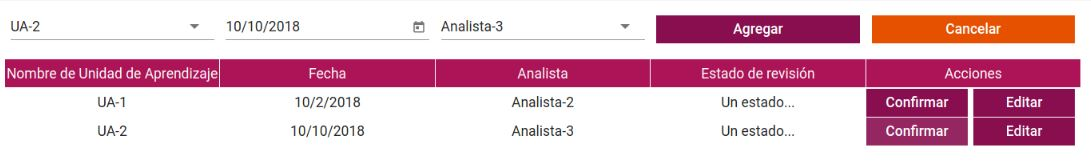
\includegraphics[width=0.7\textwidth]{DCU/SP2/Pantallas/GestionEncargado}
  \caption{SP2-IU-GestionEncargado}
  \label{SP2-IU-GestionEncargado}
\end{figure}

\chapter{SP2-CU7 Finalizar revisión de paquetes de propuestas de unidades de aprendizaje}

\begin{UseCase}{SP2-CU5}{Finalizar revisión de paquetes de propuestas de unidades de aprendizaje}{El usuario jefe de desarrollo e innovación curricular podrá aprobar un paquete de unidades de aprendizaje.}
		\UCitem{Versión}{\color{Gray}1.0}
		\UCitem{Autor}{\color{Gray}Parra Garcilazo Cinthya Dolores}
		\UCitem{Supervisa}{\color{Gray}}
		\UCitem{Actor}{\hyperlink{Usuario}{Jefe de Desarrollo e Innovación Curricular}}
		\UCitem{Propósito}{Dar por concluida la revisón de un paquete de Unidades de Aprendizaje.}
		\UCitem{Entradas}{Las entradas para el registro de una referencia bibliográfica serán:
          \begin{itemize}
          	\item Unidades de aprendizaje
          	\item Unidad Académica
            \item Semestre
            \item Analistas
          \end{itemize}
        }
		\UCitem{Origen}{Teclado, mouse.}
		\UCitem{Salidas}{
        	\begin{itemize}
        	   \item MSG. Revisión de paquete finalizada. Paquete enviado.
                \item MSG2. Error al finalizar paquete.

        	\end{itemize}
        }
		\UCitem{Destino}{Pantalla.}
		\UCitem{Precondiciones}{ Se sigue la SP2-BR10.}
		\UCitem{Postcondiciones}{El paquete es enviado a la unidad de aprendizaje correspondiete como aprobado, no se hacen más modificaciones a ninguna unidad de aprendizaje.}
		\UCitem{Errores}{}
		\UCitem{Estado}{Revisión.}
		\UCitem{Observaciones}{}
\end{UseCase}

%--------------------------- CU TRAYECTORIA PRINCIPAL -------------------------
\begin{UCtrayectoria}{Principal}


    \UCpaso Muestra la interfaz de usuario \IUref{SP2-IU-GestionPaquetes}
    \UCpaso[\UCactor] Presiona el botón \IUbutton {Finalizar}
    \UCpaso Verifica en la base de datos que todas las unidades de aprendizaje tengan el estado de revisado\hyperref[SP2-CU5-A]{Trayectoria A}.
    \UCpaso Envía notificación a la Unidad de Aprendizaje correspondiente de Paquete Aprobado. \hyperref[SP2-CU5-B]{Trayectoria B}.
    \UCpaso Muestra el mensaje \MSGref {MSG1}
    \UCpaso[\UCactor] Presiona el botón \IUbutton {Aceptar}
    \UCpaso Cambia el estado del paquete a enviado.
    \UCpaso Remueve la tabla con la información del paquete aprobado de la lista de tareas.

\end{UCtrayectoria}


%------------------------ CU TRAYECTORIA ALTERNARIVA A -------------------------
\label{SP2-CU5-A}
\begin{UCtrayectoriaA}{A}{No están todas las unidades de aprendizaje en estado de aprobado.}
    \UCpaso Muestra el mensaje \MSGref {MSG6}
    \UCpaso[\UCactor] Presiona el botón \IUbutton {Aceptar}
\end{UCtrayectoriaA}

%------------------------ CU TRAYECTORIA ALTERNARIVA B -------------------------

\label{SP2-CU5-B}
\begin{UCtrayectoriaA}{B}{No están todas las unidades de aprendizaje en estado de aprobado.}
    \UCpaso Muestra el mensaje \MSGref {MSG5}
    \UCpaso[\UCactor] Presiona el botón \IUbutton {Aceptar}
\end{UCtrayectoriaA}


%------------------------ Pantallas de este caso de uso -------------------------
\chapter{Pantallas}
 \begin{figure}
  \centering
    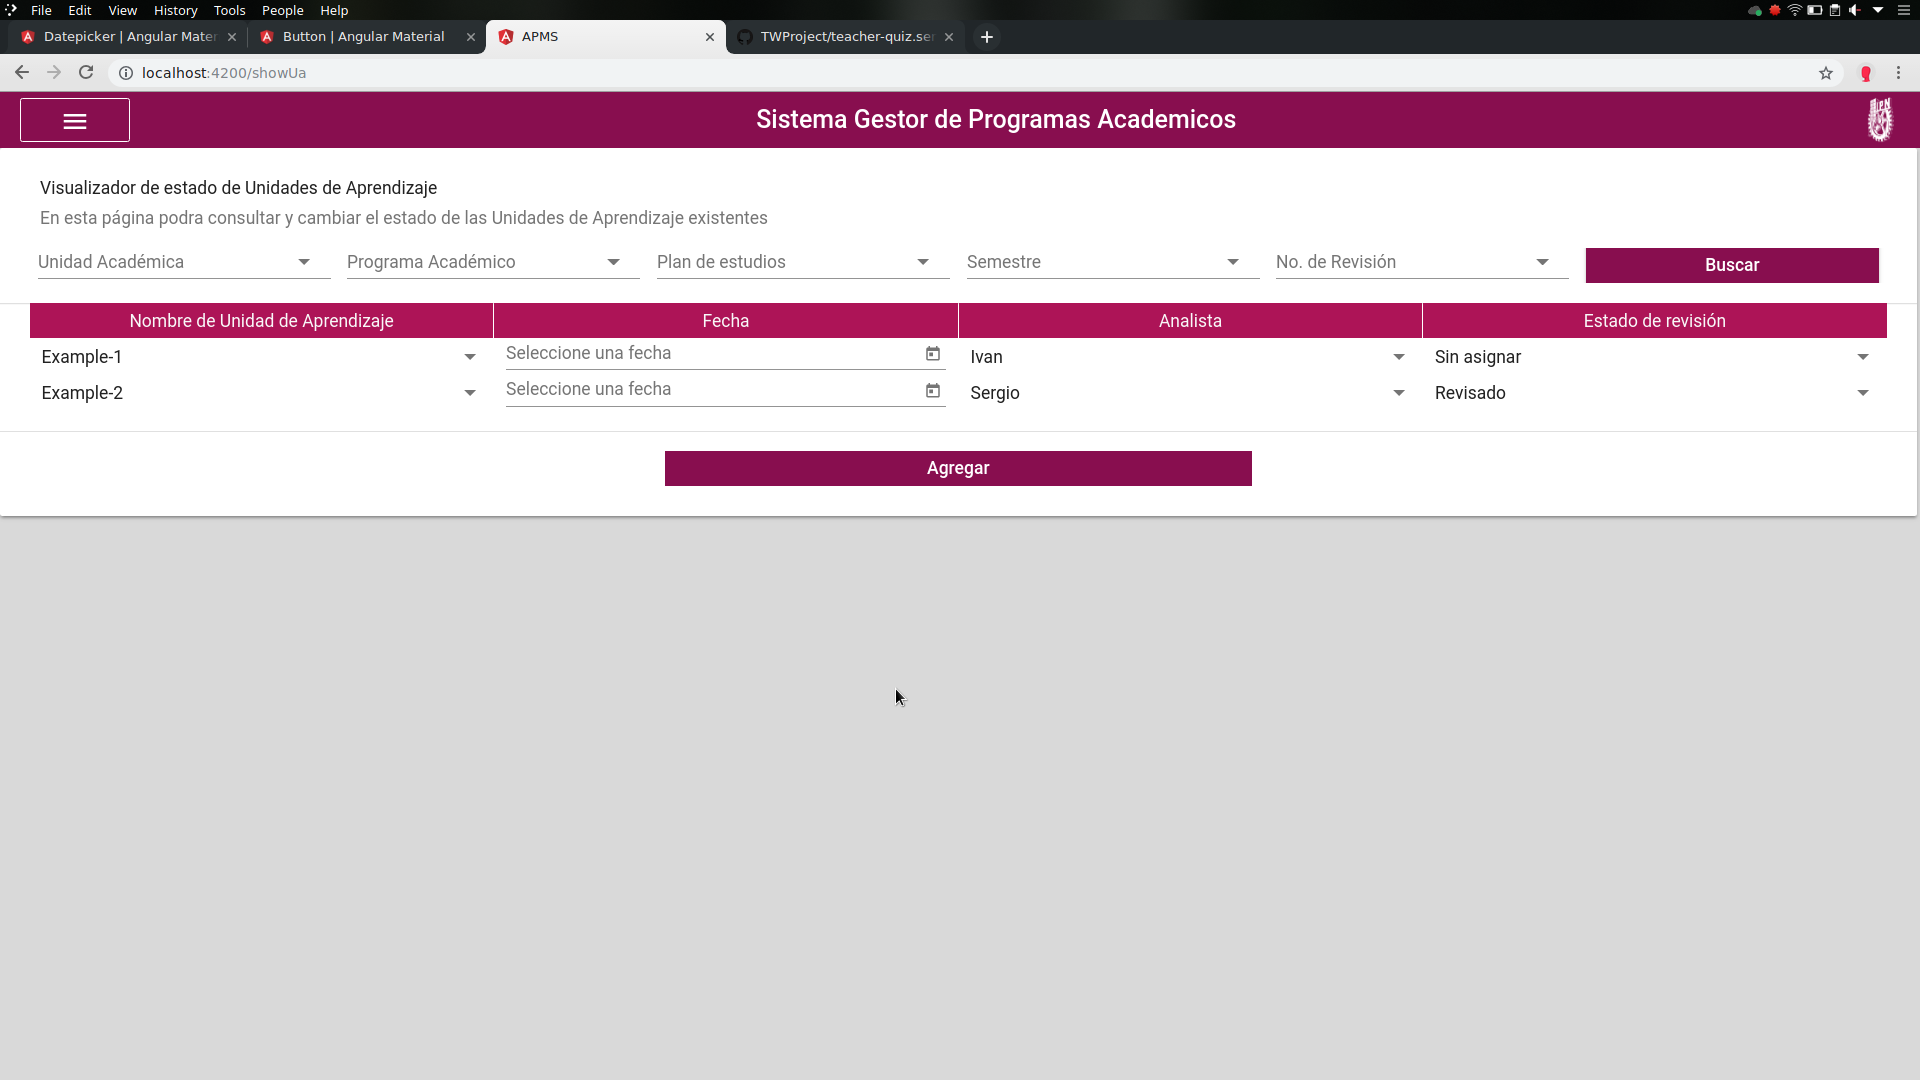
\includegraphics[width=0.7\textwidth]{DCU/SP2/Pantallas/GestionPaquetes}
  \caption{SP2-IU-GestionPaquetes}
  \label{SP2-IU-GestionPaquetes}
\end{figure}

%------------------------ Mensajes de este caso de uso -------------------------
\chapter{Pantallas}
 \begin{figure}
  \centering
    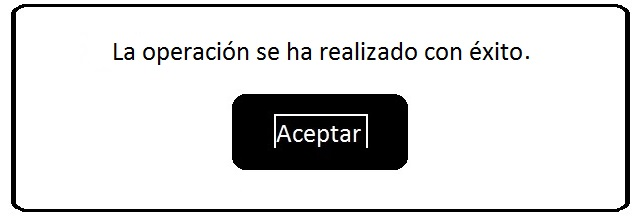
\includegraphics[width=0.7\textwidth]{DCU/SP2/mensajes/MSG1}
   \caption{SP2-MSG1}
  \label{SP2-MSG1}
\end{figure}

 \begin{figure}
  \centering
    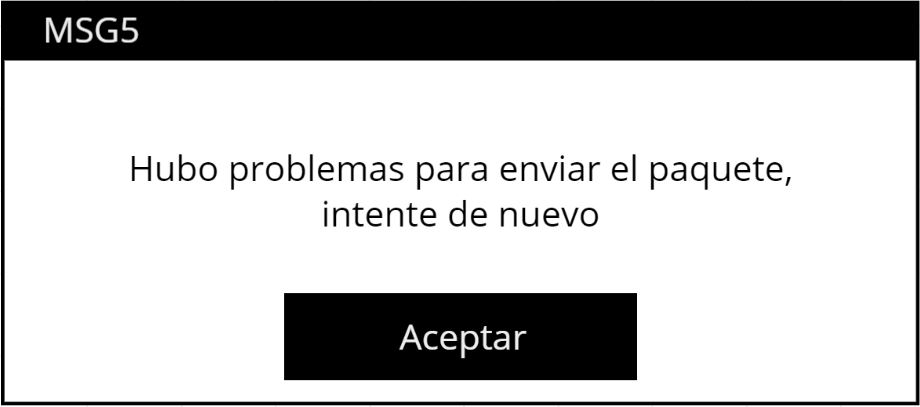
\includegraphics[width=0.7\textwidth]{DCU/SP2/mensajes/MSG5}
  \caption{SP2-MSG5}
  \label{SP2-MSG5}
\end{figure}

 \begin{figure}
  \centering
    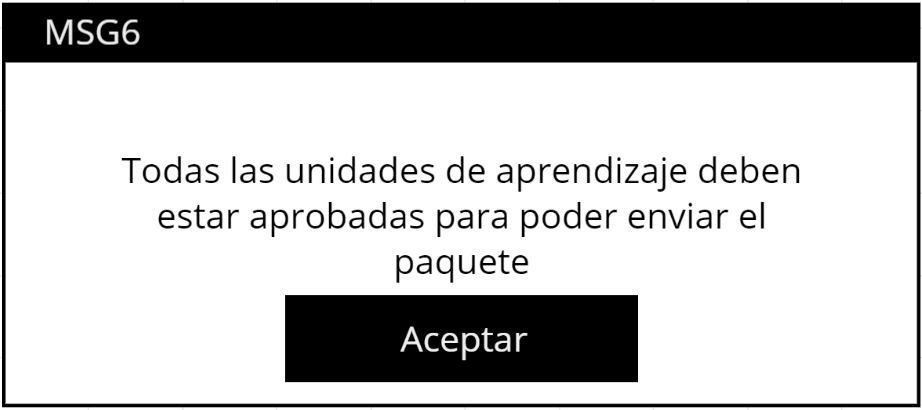
\includegraphics[width=0.7\textwidth]{DCU/SP2/mensajes/MSG6}
  \caption{SP2-MSG6}
  \label{SP2-MSG6}
\end{figure}


\chapter{Sprint 2 Autorización de seccción de Unidad de Aprendizaje}
\begin{UseCase}{SP2-CU7}{ Autorizar Sección Descripción de Unidad de Aprendizaje }{El usuario podrá registrar una o más referencias bibliográficas en el sistema.}
		\UCitem{Versión}{\color{Gray}1.0}
		\UCitem{Autor}{\color{Gray}Domínguez López Humberto}
		\UCitem{Supervisa}{\color{Gray}Parra Garcilazo Cinthya Dolores}
		\UCitem{Actor}{Analista}
		\UCitem{Propósito}{Que el analista conozca la sección de la propuesta de Unidad de Aprendizaje para determinar si necesita correcciones.}
		\UCitem{Entradas}{Clic en botones:
          \begin{itemize}
          	\item Finalizar Revisión.
          	\item Guardar.
            \item Cancelar.
            \item Nuevo Comentario.
            \item Subrayar.
            \item Eliminar subrayado.
            \item Editar Comentario.
            \item Eliminar Comentario.
          \end{itemize}
        }
		\UCitem{Origen}{Mouse.}
		\UCitem{Salidas}{
        	\begin{itemize}
        		\item MSG15. ¿Está seguro que desea Cancelar la revisión?
				Se perderán las Anotaciones que no hayas guardado anteriormente.
               \item MSG16. ¿Está seguro de Finalizar la Revisión?
               \item MSG17 Sección Aprobada.
                
               \item MSG18 Revisión de Sección Finalizada.
               \item MSG19 Anotaciones En Sección Guardadas Correctamente.

        	\end{itemize}
        }
		\UCitem{Destino}{Pantalla.}
		\UCitem{Precondiciones}{ Se llamó el caso de uso SP2-CU1}
		\UCitem{Postcondiciones}{Se habilita la llamada a los casos de uso SP2-CU14, SP2-CU15, SP2-CU16, SP2-CU17.}
		\UCitem{Errores}{}
		\UCitem{Estado}{Revisión.}
		\UCitem{Observaciones}{}
\end{UseCase}

%--------------------------- CU TRAYECTORIA PRINCIPAL -------------------------
\begin{UCtrayectoria}{Principal}

    \UCpaso[\UCactor] presiona el botón  \IUbutton{Descripción} de la interfaz de usuario \IUref{SP2-IU-INICIO}{Sección Inicio}

    \UCpaso El sistema obtiene la información correspondiente a la sección de descripción.
    
    \UCpaso El sistema obtiene la bitácora de comentarios correspondientes a la sección de la Unidad de Aprendizaje. 
    
    \UCpaso El sistema verifica que la sección de la Unidad de Aprendizaje no haya sido aprobada anteriormente. \BRref{BR9}{Aprobación de Tareas Seccionadas.} \hyperlink{SP2-CU7-A1}{Trayectoria A1}. 
    
    \UCpaso El sistema muestra la interfaz de usuario \IUref{SP2-IU-DESCRIPCION}{Sección Descripción} .
    
    \UCpaso[\UCactor] presiona el botón \IUbutton{Finalizar Revisión}. \hyperlink{SP2-CU7-A2}{Trayectoria A2}.
    \UCpaso El sistema muestra el \MSGref{MSG16}{¿Está seguro de Finalizar la Revisión?}.
    
    \UCpaso	El sistema verifica que no existan nuevos comentarios o subrayados para la sección de la Unidad de Aprendizaje.\BRref{BR8}{Aprobación de Tareas.}\hyperlink{SP2-CU7-A3}{Trayectoria A3}. 
    
    \UCpaso El sistema pone el estado de la sección Descripción  en “Aprobado”.
    
    \UCpaso El sistema muestra el mensaje \MSGref{MSG17}{Sección Aprobada}.

    \UCpaso El sistema muestra la interfaz de usuario \IUref{SP2-IU-INICIO}{Sección Inicio}

\end{UCtrayectoria}

%------------------------ CU TRAYECTORIA ALTERNARIVA A1 -------------------------

\begin{UCtrayectoriaA}{A1}{La sección de la Unidad de Aprendizaje ya ha sido aprobada anteriormente.}

	\hypertarget{SP2-CU7-A1}{\UCpaso El sistema muestra la interfaz de usuario \IUref{SP2-IU-DESCRIPCION}{Sección Descripción}}
    \UCpaso El sistema deshabilita los botones superiores: \IUbutton{Nuevo Comentario}, \IUbutton{Subrayar}, \IUbutton{Eliminar Subrayado}.
    \UCpaso El sistema deshabilita los botones inferiores: \IUbutton{Cancelar}, \IUbutton{Guardar}, \IUbutton{Finalizar Revisión}.
    \UCpaso El sistema deshabilita los botones laterales de: \IUbutton{Modificar Comentario}, \IUbutton{Eliminar Comentario}.
\end{UCtrayectoriaA}

%------------------------ CU TRAYECTORIA ALTERNARIVA A2 -------------------------
	
\begin{UCtrayectoriaA}{A2}{El analista no desea finalizar aun la revisión de la sección de la Unidad de Aprendizaje.}

    \hypertarget{SP2-CU7-A2}{\UCpaso[\UCactor] presiona el botón \IUbutton{Guardar} \hyperlink{SP2-CU7-A2.1}{Trayectoria A2.1}}. 
    \UCpaso El sistema guarda los nuevos comentaros y subrayados hechos durante esa sesión.
    \UCpaso El sistema muestra el mensaje \MSGref{MSG19}{Anotaciones En Sección Guardadas Correctamente}.
    \UCpaso El sistema muestra la interfaz de usuario \IUref{SP2-IU-INICIO}{Sección Inicio}
\end{UCtrayectoriaA}

%------------------------ CU TRAYECTORIA ALTERNARIVA A2.1 -----------------------
\begin{UCtrayectoriaA}{A2.1}{El analista desea cancelar todo lo que haya hecho en la sección de la Unidad de Aprendizaje durante esa sesión.}

	\hypertarget{SP2-CU7-A2.1}{\UCpaso[\UCactor] presiona el botón \IUbutton{Cancelar}}. 
    \UCpaso El sistema muestra el mensaje \MSGref{MSG15}{¿Está seguro que desea Cancelar la revisión? Se perderán las Anotaciones que no hayas guardado anteriormente.}
Se perderán las Anotaciones que no hayas guardado anteriormente. .
    \UCpaso El sistema elimina los nuevos comentaros y subrayados hechos durante esa sesión.
    \UCpaso El sistema muestra la interfaz de usuario \IUref{SP2-IU-INICIO}{Sección Inicio}.
\end{UCtrayectoriaA}

%------------------------ CU TRAYECTORIA ALTERNARIVA A3 -----------------------
	
\begin{UCtrayectoriaA}{A3}{El analista realizo comentarios y subrayados para su posterior corrección en la sección de la Unidad de Aprendizaje.} 

	\hypertarget{SP2-CU7-A3}{\UCpaso El sistema pone el estado de la sección Descripción de Unidad de Aprendizaje en “Revisado”.}
    \UCpaso El sistema muestra el mensaje \MSGref{MSG18}{Revisión de Sección Finalizada}.
    \UCpaso El sistema muestra la interfaz de usuario \IUref{SP2-IU-INICIO}{Sección Inicio}.
\end{UCtrayectoriaA}
\chapter{SP2-CU8 Autorizar Sección Tiempos Asignados de Unidad de Aprendizaje}
\begin{UseCase}{SP2-CU8}{ Autorizar Sección Tiempos Asignados de Unidad de Aprendizaje}{El analista podrá visualizar la información de la sección de tiempos asignados de la unidad de aprendizaje para poder aprobarla.}
		\UCitem{Versión}{\color{Gray}1.0}
		\UCitem{Autor}{\color{Gray}Domínguez López Humberto}
		\UCitem{Supervisa}{\color{Gray}Parra Garcilazo Cinthya Dolores}
		\UCitem{Actor}{Analista}
		\UCitem{Propósito}{Que el analista conozca la sección de Tiempos Asignados de la propuesta de Unidad de Aprendizaje para determinar si necesita correcciones.}
		\UCitem{Entradas}{Clic en botones:
          \begin{itemize}
          	\item Finalizar Revisión.
          	\item Guardar.
            \item Cancelar.
            \item Nuevo Comentario.
            \item Subrayar.
            \item Eliminar subrayado.
            \item Editar Comentario.
            \item Eliminar Comentario.
          \end{itemize}
        }
		\UCitem{Origen}{Mouse.}
		\UCitem{Salidas}{
        	\begin{itemize}
        		\hypertarget{MSG1}{\item MSG1. ¿Está seguro que desea Cancelar la revisión?
				Se perderán las Anotaciones que no hayas guardado anteriormente.}
                \hypertarget{MSG2}{\item MSG2. ¿Está seguro de Finalizar la Revisión?}
                \hypertarget{MSG3}{\item MSG3 Sección Aprobada.}
                
               \hypertarget{MSG4}{ \item MSG4 Revisión de Sección Finalizada.}
                \hypertarget{MSG5}{\item MSG5 Anotaciones En Sección Guardadas Correctamente.}

        	\end{itemize}
        }
		\UCitem{Destino}{Pantalla.}
		\UCitem{Precondiciones}{ Se llamó el caso de uso SP2-CU1}
		\UCitem{Postcondiciones}{Se habilita la llamada a los casos de uso SP2-CU14, SP2-CU15, SP2-CU16, SP2-CU17.}
		\UCitem{Errores}{}
		\UCitem{Estado}{Revisión.}
		\UCitem{Observaciones}{}
\end{UseCase}

%--------------------------- CU TRAYECTORIA PRINCIPAL -------------------------
\begin{UCtrayectoria}{Principal}

    \UCpaso[\UCactor] presiona el botón  \IUbutton{Tiempos Asignados} de la interfaz de usuario \IUref{SP2-IU-INICIO}{Sección Inicio}

    \UCpaso El sistema obtiene la información correspondiente a la sección de Tiempos Asignados.
    
    \UCpaso El sistema obtiene la bitácora de comentarios correspondientes a la sección Tiempos Asignados de la Unidad de Aprendizaje. 
    
    \UCpaso El sistema verifica que la sección Tiempos Asignados de la Unidad de Aprendizaje no haya sido aprobada anteriormente. Regla de Negocio SP2-BR7. \hyperlink{SP2-CU8-A1}{Trayectoria A1}. 
    
    \UCpaso El sistema muestra la interfaz de usuario  \IUref{SP2-IU-TIEMPOS}{Sección Tiempos Asignados}.
    
    \UCpaso[\UCactor] presiona el botón \IUbutton{Finalizar Revisión}. \hyperlink{SP2-CU8-A2}{Trayectoria A2}.
    \UCpaso El sistema muestra el \MSGref{MSG2}{¿Está seguro de Finalizar la Revisión?}.
    
    \UCpaso	El sistema verifica que no existan nuevos comentarios o subrayados para la sección de la Unidad de Aprendizaje. Regla de Negocio  SP2-BR1 \hyperlink{SP2-CU8-A3}{Trayectoria A3}. 
    
    \UCpaso El sistema pone el estado de la sección Tiempos Asignados  en “Aprobado”.
    
    \UCpaso El sistema muestra el mensaje \MSGref{MSG3}{Sección Aprobada}.

    \UCpaso El sistema muestra la interfaz de usuario \IUref{SP2-IU-INICIO}{Sección Inicio}

\end{UCtrayectoria}

%------------------------ CU TRAYECTORIA ALTERNARIVA A1 -------------------------

\begin{UCtrayectoriaA}{A1}{La sección de la Unidad de Aprendizaje ya ha sido aprobada anteriormente.}

	\hypertarget{SP2-CU8-A1}{\UCpaso El sistema muestra la interfaz de usuario \IUref{SP2-IU-TIEMPOS}{Sección Tiempos Asignados}.}
    \UCpaso El sistema deshabilita los botones superiores: \IUbutton{Nuevo Comentario}, \IUbutton{Subrayar}, \IUbutton{Eliminar Subrayado}.
    \UCpaso El sistema deshabilita los botones inferiores: \IUbutton{Cancelar}, \IUbutton{Guardar}, \IUbutton{Finalizar Revisión}.
    \UCpaso El sistema deshabilita los botones laterales de: \IUbutton{Modificar Comentario}, \IUbutton{Eliminar Comentario}.
\end{UCtrayectoriaA}

%------------------------ CU TRAYECTORIA ALTERNARIVA A2 -------------------------
	
\begin{UCtrayectoriaA}{A2}{El analista no desea finalizar aun la revisión de la sección de la Unidad de Aprendizaje.}

    \hypertarget{SP2-CU8-A2}{\UCpaso[\UCactor] presiona el botón \IUbutton{Guardar} \hyperlink{SP2-CU8-A2.1}{Trayectoria A2.1}}. 
    \UCpaso El sistema guarda los nuevos comentaros y subrayados hechos durante esa sesión.
    \UCpaso El sistema muestra el mensaje \MSGref{MSG5}{Anotaciones En Sección Guardadas Correctamente}.
    \UCpaso El sistema muestra la interfaz de usuario \IUref{SP2-IU-INICIO}{Sección Inicio}
\end{UCtrayectoriaA}

%------------------------ CU TRAYECTORIA ALTERNARIVA A2.1 -----------------------
\begin{UCtrayectoriaA}{A2.1}{El analista desea cancelar todo lo que haya hecho en la sección de la Unidad de Aprendizaje durante esa sesión.}

	\hypertarget{SP2-CU8-A2.1}{\UCpaso[\UCactor] presiona el botón \IUbutton{Cancelar}}. 
    \UCpaso El sistema muestra el mensaje \MSGref{MSG1}{¿Está seguro que desea Cancelar la revisión? Se perderán las Anotaciones que no hayas guardado anteriormente.}
Se perderán las Anotaciones que no hayas guardado anteriormente. .
    \UCpaso El sistema elimina los nuevos comentaros y subrayados hechos durante esa sesión.
    \UCpaso El sistema muestra la interfaz de usuario \IUref{SP2-IU-INICIO}{Sección Inicio}.
\end{UCtrayectoriaA}

%------------------------ CU TRAYECTORIA ALTERNARIVA A3 -----------------------
	
\begin{UCtrayectoriaA}{A3}{El analista realizo comentarios y subrayados para su posterior corrección en la sección de la Unidad de Aprendizaje.} 

	\hypertarget{SP2-CU8-A3}{\UCpaso El sistema pone el estado de la sección Descripción de Unidad de Aprendizaje en “Revisado”.}
    \UCpaso El sistema muestra el mensaje \MSGref{MSG4}{Revisión de Sección Finalizada}.
    \UCpaso El sistema muestra la interfaz de usuario \IUref{SP2-IU-INICIO}{Sección Inicio}.
\end{UCtrayectoriaA}

\chapter{Pantallas}
\IUfig[0.75]{SP2-Pantallas/Inicio}{SP2-IU-INICIO}{Sección Inicio}
\IUfig[0.75]{SP2-Pantallas/Tiempos_Asignados}{SP2-IU-TIEMPOS}{Sección Tiempos Asignados}


\begin{UseCase}{SP2-CU9}{ Autorizar Sección Perfil Docente de Unidad de Aprendizaje}{El analista podrá visualizar la información de la sección de Perfil Docente  de la unidad de aprendizaje para poder aprobarla.} 
		\UCitem{Versión}{\color{Gray}1.0}
		\UCitem{Autor}{\color{Gray}Domínguez López Humberto}
		\UCitem{Supervisa}{\color{Gray}Parra Garcilazo Cinthya Dolores}
		\UCitem{Actor}{Analista}
		\UCitem{Propósito}{Que el analista conozca la sección de Perfil Docente de la propuesta de Unidad de Aprendizaje para determinar si necesita correcciones.}
		\UCitem{Entradas}{Clic en botones:
          \begin{itemize}
          	\item Finalizar Revisión.
          	\item Guardar.
            \item Cancelar.
            \item Nuevo Comentario.
            \item Subrayar.
            \item Eliminar subrayado.
            \item Editar Comentario.
            \item Eliminar Comentario.
          \end{itemize}
        }
		\UCitem{Origen}{Mouse.}
		\UCitem{Salidas}{
        	\begin{itemize}
        			\item MSG15. ¿Está seguro que desea Cancelar la revisión?
				Se perderán las Anotaciones que no hayas guardado anteriormente.
               \item MSG16. ¿Está seguro de Finalizar la Revisión?
               \item MSG17 Sección Aprobada.
                
               \item MSG18 Revisión de Sección Finalizada.
               \item MSG19 Anotaciones En Sección Guardadas Correctamente.

        	\end{itemize}
        }
		\UCitem{Destino}{Pantalla.}
		\UCitem{Precondiciones}{ Se llamó el caso de uso SP2-CU1}
		\UCitem{Postcondiciones}{Se habilita la llamada a los casos de uso SP2-CU11, SP2-CU14.}
		\UCitem{Errores}{}
		\UCitem{Estado}{Revisión.}
		\UCitem{Observaciones}{}
\end{UseCase}

%--------------------------- CU TRAYECTORIA PRINCIPAL -------------------------
\begin{UCtrayectoria}{Principal}

    \UCpaso[\UCactor] presiona el botón  \IUbutton{Perfil Docente} de la interfaz de usuario \IUref{SP2-IU-INICIO}{Sección Inicio}

    \UCpaso El sistema obtiene la información correspondiente a la sección de Perfil Docente.
    
    \UCpaso El sistema obtiene la bitácora de comentarios correspondientes a la sección Perfil Docente de la Unidad de Aprendizaje. 
    
    \UCpaso El sistema verifica que la sección Perfil Docente de la Unidad de Aprendizaje no haya sido aprobada anteriormente. \BRref{BR9}{Aprobación de Tareas Seccionadas.} \hyperlink{SP2-CU9-A1}{Trayectoria A1}. 
    
    \UCpaso El sistema muestra la interfaz de usuario  \IUref{SP2-IU-Perfil-Docente}{Sección Perfil Docente}. 
    
    \UCpaso[\UCactor] presiona el botón \IUbutton{Finalizar Revisión}. \hyperlink{SP2-CU9-A2}{Trayectoria A2}.
    \UCpaso El sistema muestra el \MSGref{MSG16}{¿Está seguro de Finalizar la Revisión?}.
    
    \UCpaso	El sistema verifica que no existan nuevos comentarios o subrayados para la sección de la Unidad de Aprendizaje. \BRref{BR8}{Aprobación de Tareas.} \hyperlink{SP2-CU9-A3}{Trayectoria A3}. 
    
    \UCpaso El sistema pone el estado de la sección Perfil Docente en “Aprobado”.
    
    \UCpaso El sistema muestra el mensaje \MSGref{MSG17}{Sección Aprobada}.

    \UCpaso El sistema muestra la interfaz de usuario \IUref{SP2-IU-INICIO}{Sección Inicio}

\end{UCtrayectoria}

%------------------------ CU TRAYECTORIA ALTERNARIVA A1 -------------------------

\begin{UCtrayectoriaA}{A1}{La sección de la Unidad de Aprendizaje ya ha sido aprobada anteriormente.}

	\hypertarget{SP2-CU9-A1}{\UCpaso El sistema muestra la interfaz de usuario \IUref{SP2-IU-Perfil-Docente}{Sección Perfil Docente}.}
    \UCpaso El sistema deshabilita los botones superiores: \IUbutton{Nuevo Comentario}, \IUbutton{Subrayar}, \IUbutton{Eliminar Subrayado}.
    \UCpaso El sistema deshabilita los botones inferiores: \IUbutton{Cancelar}, \IUbutton{Guardar}, \IUbutton{Finalizar Revisión}.
    \UCpaso El sistema deshabilita los botones laterales de: \IUbutton{Modificar Comentario}, \IUbutton{Eliminar Comentario}.
\end{UCtrayectoriaA}

%------------------------ CU TRAYECTORIA ALTERNARIVA A2 -------------------------
	
\begin{UCtrayectoriaA}{A2}{El analista no desea finalizar aun la revisión de la sección de la Unidad de Aprendizaje.}

    \hypertarget{SP2-CU9-A2}{\UCpaso[\UCactor] presiona el botón \IUbutton{Guardar} \hyperlink{SP2-CU9-A2.1}{Trayectoria A2.1}}. 
    \UCpaso El sistema guarda los nuevos comentaros y subrayados hechos durante esa sesión.
    \UCpaso El sistema muestra el mensaje \MSGref{MSG19}{Anotaciones En Sección Guardadas Correctamente}.
    \UCpaso El sistema muestra la interfaz de usuario \IUref{SP2-IU-INICIO}{Sección Inicio}
\end{UCtrayectoriaA}

%------------------------ CU TRAYECTORIA ALTERNARIVA A2.1 -----------------------
\begin{UCtrayectoriaA}{A2.1}{El analista desea cancelar todo lo que haya hecho en la sección de la Unidad de Aprendizaje durante esa sesión.}

	\hypertarget{SP2-CU9-A2.1}{\UCpaso[\UCactor] presiona el botón \IUbutton{Cancelar}}. 
    \UCpaso El sistema muestra el mensaje \MSGref{MSG15}{¿Está seguro que desea Cancelar la revisión? Se perderán las Anotaciones que no hayas guardado anteriormente.}
Se perderán las Anotaciones que no hayas guardado anteriormente. .
    \UCpaso El sistema elimina los nuevos comentaros y subrayados hechos durante esa sesión.
    \UCpaso El sistema muestra la interfaz de usuario \IUref{SP2-IU-INICIO}{Sección Inicio}.
\end{UCtrayectoriaA}

%------------------------ CU TRAYECTORIA ALTERNARIVA A3 -----------------------
	
\begin{UCtrayectoriaA}{A3}{El analista realizo comentarios y subrayados para su posterior corrección en la sección de la Unidad de Aprendizaje.} 

	\hypertarget{SP2-CU9-A3}{\UCpaso El sistema pone el estado de la sección Perfil Docente de Unidad de Aprendizaje en “Revisado”.}
    \UCpaso El sistema muestra el mensaje \MSGref{MSG18}{Revisión de Sección Finalizada}.
    \UCpaso El sistema muestra la interfaz de usuario \IUref{SP2-IU-INICIO}{Sección Inicio}.
\end{UCtrayectoriaA}
\chapter{SP2-CU14 Agregar comentarios a propuesta de unidad de aprendizaje}
\begin{UseCase}{SP2-CU14}{ Agregar comentarios a propuesta de unidad de aprendizaje }{El usuario podrá agregar uno o más comentarios en la sección de propuesta de unidad de aprendizaje que está revisando.}
		\UCitem{Versión}{\color{Gray}1.0}
		\UCitem{Autor}{\color{Gray}Romero Ponce Mauricio Isaac}
		\UCitem{Supervisa}{\color{Gray}Parra Garcilazo Cinthya Dolores}
		\UCitem{Actor}{Analista}
		\UCitem{Propósito}{Asignar cuales son y donde están las correcciones que se deben realizar a la sección de la unidad de aprendizaje que se está revisando.}
		\UCitem{Entradas}{Las dos entradas para agregar un comentario en una sección de la propuesta de unidad de aprendizaje son:
          \begin{itemize}
          	\item Posición en la que se agregará el comentario.
          	\item Comentario.
           % \item fecha en que se genera el nuevo comentario.
            %\item Identificador unico del analista.
          \end{itemize}
        }
		\UCitem{Origen}{Mouse y teclado.}
		\UCitem{Salidas}{
        	\begin{itemize}
        		\item MSG1. La operación se ha realizado con éxito.

                \item MSG2. Error: Primero se debe seleccionar el punto en donde se agregará el comentario.
                \item MSG3 Error: debe agregar un texto al nuevo comentario.
                \item MSG4 Ingrese su comentario en el nuevo campo de la bitácora.
        	\end{itemize}
        }
		\UCitem{Destino}{Pantalla.}
		\UCitem{Precondiciones}{ Se llamó el caso de uso SP2-CU7 o SP2-CU8 o SP2-CU9 o SP2-CU10 o  SP2-CU11 o o SP2-CU12}
		\UCitem{Postcondiciones}{
            \begin{itemize}
                \item Se agregará al sistema el comentario.
                \item Se mostrará en la bitácora el comentario
                \item Se habilita la llamada a los casos de uso SP2-CU15 y SP2-CU16  
             \end{itemize}  
        }
		\UCitem{Errores}{}
		\UCitem{Estado}{Revisión.}
		\UCitem{Observaciones}{}
\end{UseCase}

%--------------------------- CU TRAYECTORIA PRINCIPAL -------------------------
\begin{UCtrayectoria}{Principal}

    \UCpaso[\UCactor] Selecciona con el mouse el texto donde pondrá un comentario.

    \UCpaso[\UCactor] Presiona el botón \IUbutton{Nuevo comentario}. \hyperref[SP2-CU14-A]{Trayectoria A}. 
    
    \UCpaso Obtiene la fecha de la fecha actual. 
    
    \UCpaso Obtiene la clave del usuario que desea agregar un comentario.
    
    \UCpaso Muestra el nuevo comentario en el costado derecho del documento a la altura en que se seleccionó el texto del paso 1. \hyperref[SP2-CU14-B]{Trayectoria B}.
    
    \UCpaso Muestra el mensaje \MSGref{MSG4}.

    \UCpaso[\UCactor] Cierra el mensaje presionando \IUbutton{Aceptar}.
    
    \UCpaso[\UCactor] Ingresa el nuevo comentario en el input text "comentario".
    
    \UCpaso[\UCactor] Presiona el botón \IUbutton{Aceptar}. \hyperref[SP2-CU14-C]{Trayectoria C}.
    
    \UCpaso Verifica que el campo comentario haya sido contestado. \hyperref[SP2-CU14-D]{Trayectoria D}.

    \UCpaso Guarda la información del nuevo comentario en la base de datos.

    \UCpaso El sistema muestra el  \MSGref{MSG1}.

    \UCpaso[\UCactor] Cierra el mensaje presionando \IUbutton{Aceptar}.

    \UCpaso desaparecen los botones  \IUbutton{Aceptar} y  \IUbutton{Cancelar}.

    \UCpaso Aparecen los botones  \IUbutton{Editar} y  \IUbutton{Eliminar}.

\end{UCtrayectoria}

%------------------------ CU TRAYECTORIA ALTERNARIVA A -------------------------
\label{SP2-CU14-A}
\begin{UCtrayectoriaA}{A}{El usuario no seleccionó alguna parte del texto.}

	\UCpaso El sistema detecta que no hay referencia en el texto para el nuevo comentario.

  \UCpaso El sistema muestra el \MSGref{MSG2}.

  \UCpaso[\UCactor] Cierra el mensaje presionando \IUbutton{Aceptar}.

  \UCpaso continúa en el paso 1 de la trayectoria principal del CU-V14.
\end{UCtrayectoriaA}

%------------------------ CU TRAYECTORIA ALTERNARIVA B -------------------------
\label{SP2-CU14-B}
\begin{UCtrayectoriaA}{B}{El sistema detecta un comentario ya existente en el mismo renglón que el nuevo comentario.}

    \UCpaso Genera el comentario nuevo debajo del comentario ya existente. 
    \UCpaso continúa en el paso 6 de la trayectoria principal del CU-V14.
\end{UCtrayectoriaA}

%------------------------ CU TRAYECTORIA ALTERNARIVA C -----------------------
\label{SP2-CU14-C}
\begin{UCtrayectoriaA}{C}{El usuario presionó \IUbutton{Cancelar}}

	\UCpaso Elimina el comentario generado previamente.
\end{UCtrayectoriaA}

%------------------------ CU TRAYECTORIA ALTERNARIVA D -----------------------
\label{SP2-CU14-D}
\begin{UCtrayectoriaA}{D}{El sistema detecta que el campo “comentario” se encuentra vacío.} 

	\UCpaso Muestra el \MSGref{MSG3}.
    \UCpaso El sistema muestra el mensaje \MSGref{MSG4}.

    \UCpaso[\UCactor] Cierra el mensaje presionando \IUbutton{Aceptar}.

    \UCpaso Continúa en el paso 8 de la trayectoria principal del CU-V14.
\end{UCtrayectoriaA}

\chapter{Pantallas}
 \begin{figure}
  \centering
    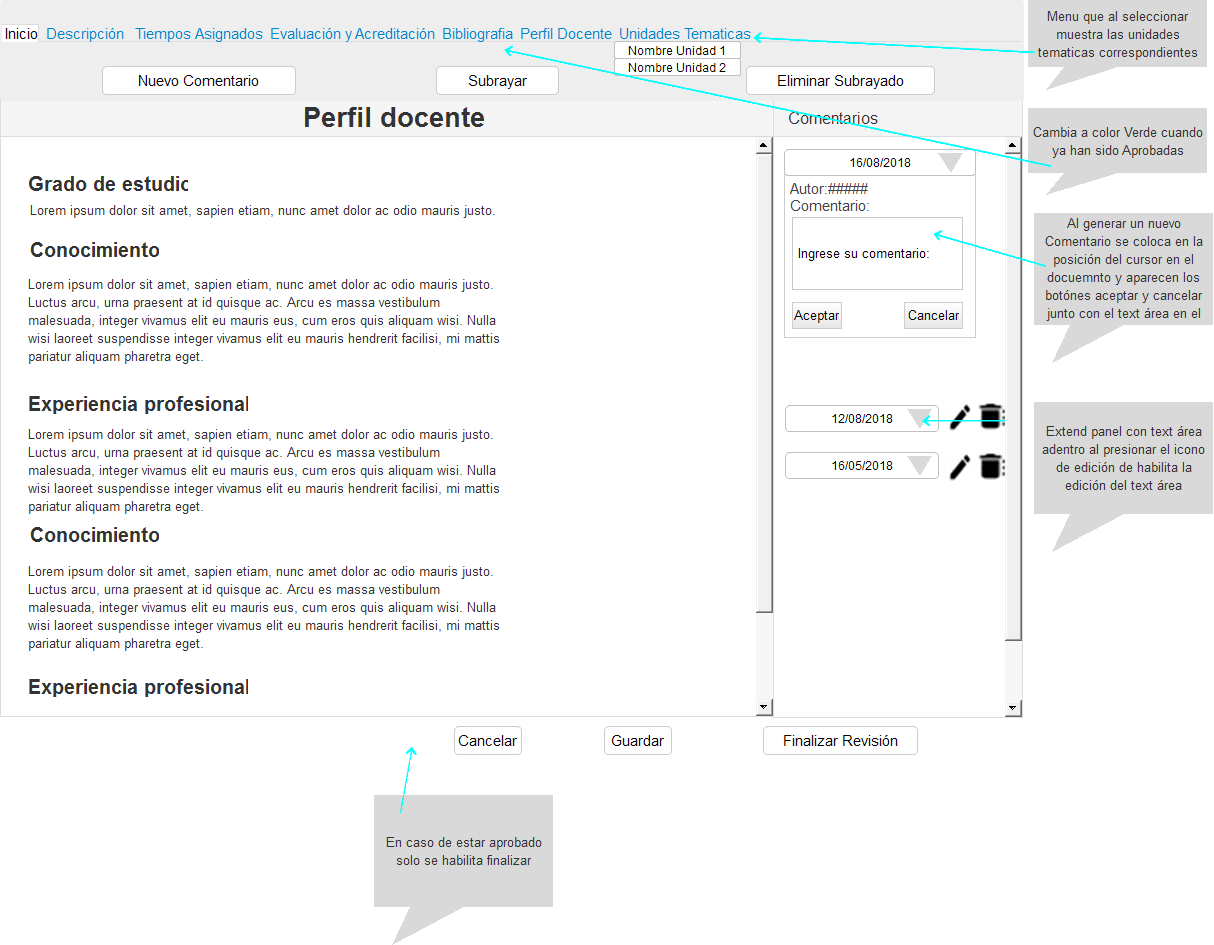
\includegraphics[width=0.7\textwidth]{DCU/SP2/Pantallas/Nuevo_comentario}
  \caption{SP2-IU-Nuevo comentario}
  \label{SP2-IU-Nuevo_comentario}
\end{figure}

\chapter{SP2-CU15 Modificar comentarios a propuesta de Unidad de Aprendizaje}
\begin{UseCase}{SP2-CU15}{ Modificar comentarios a propuesta de Unidad de Aprendizaje }{El usuario podrá modificar los comentarios previamente realizados en la sección de propuesta de Unidad de Aprendizaje que se está revisando.}
		\UCitem{Versión}{\color{Gray}1.0}
		\UCitem{Autor}{\color{Gray}Romero Ponce Mauricio Isaac}
		\UCitem{Supervisa}{\color{Gray}Parra Garcilazo Cinthya Dolores}
		\UCitem{Actor}{Analista}
		\UCitem{Propósito}{Tener oportunidad de modificar el contenido de los comentarios generados previamente en la propuesta de Unidad de Aprendizaje.}
		\UCitem{Entradas}{Las unica entrada para modificar un comentario en una sección de la propuesta de Unidad de Aprendizaje es:
          \begin{itemize}
          	\item Modificación al comentario anterior.
           % \item fecha en que se genera el nuevo comentario.
            %\item Identificador unico del analista.
          \end{itemize}
        }
		\UCitem{Origen}{Mouse y teclado.}
		\UCitem{Salidas}{
        	\begin{itemize}
        		\hypertarget{CU15-MSG1}{\item MSG1 La operación se ha realizado con éxito.}
            \hypertarget{CU15-MSG3}{\item MSG3 Error: debe agregar un texto al nuevo comentario.}
            \hypertarget{CU15-MSG4}{\item MSG4 Ingrese su comentario en el nuevo campo de la bitácora.}
        	\end{itemize}
        }
		\UCitem{Destino}{Pantalla.}
		\UCitem{Precondiciones}{ Se llamó al caso de uso SP2-CU14}
		\UCitem{Postcondiciones}{
            \begin{itemize}
                \item Se modificará en el sistema el comentario.
                \item Se modificará en el sistema la fecha del comentario.
                \item Se mostrará en la bitácora la modificación del comentario.  
             \end{itemize}  
        }
		\UCitem{Errores}{}
		\UCitem{Estado}{Revisión.}
		\UCitem{Observaciones}{}
\end{UseCase}

%--------------------------- CU TRAYECTORIA PRINCIPAL -------------------------
\begin{UCtrayectoria}{Principal}


    \UCpaso[\UCactor] Presiona el botón \IUbutton{Modificar comentario}. 
    
    \UCpaso Obtiene la fecha actual. 
    
    \UCpaso Muestra el mensaje \MSGref{CU15-MSG4}{Ingrese su comentario en el nuevo campo de la bitácora.}.

    \UCpaso[\UCactor] Cierra el mensaje presionando \IUbutton{Aceptar}.
    
    \UCpaso[\UCactor] Ingresa el nuevo comentario en el input text "comentario".
    
    \UCpaso[\UCactor] Presiona el botón \IUbutton{Aceptar}. \hyperref[SP2-CU15-A]{Trayectoria A}.
    
    \UCpaso Verifica que el campo comentario haya sido contestado. \hyperref[SP2-CU15-B]{Trayectoria B}.

    \UCpaso Actualiza la fecha del comentario en el sistema al que se presionó el botón \IUbutton{Modificar comentario}.

    \UCpaso Guarda la modificación del comentario en el sistema.

    \UCpaso El sistema muestra el  \MSGref{CU15-MSG1}{La operación se ha realizado con éxito.}.

    \UCpaso[\UCactor] Cierra el mensaje presionando \IUbutton{Aceptar}.


\end{UCtrayectoria}

%------------------------ CU TRAYECTORIA ALTERNARIVA A -------------------------

\label{SP2-CU15-A}
\begin{UCtrayectoriaA}{A}{El usuario presionó \IUbutton{Cancelar}}

  \UCpaso Deja el comentario sin modificaciones.
\end{UCtrayectoriaA}

%------------------------ CU TRAYECTORIA ALTERNARIVA B -------------------------
\label{SP2-CU15-B}
\begin{UCtrayectoriaA}{B}{El sistema detecta que el campo “comentario” se encuentra vacío.} 
    \UCpaso El sistema muestra el mensaje \MSGref{CU15-MSG3}{Error: debe agregar un texto al nuevo comentario.}.
    \UCpaso[\UCactor] Cierra el mensaje presionando \IUbutton{Aceptar}.
    \UCpaso Continúa en el paso 6 de la trayectoria principal del SP2-CU15.
\end{UCtrayectoriaA}

\chapter{Pantallas}
 \begin{figure}
  \centering
    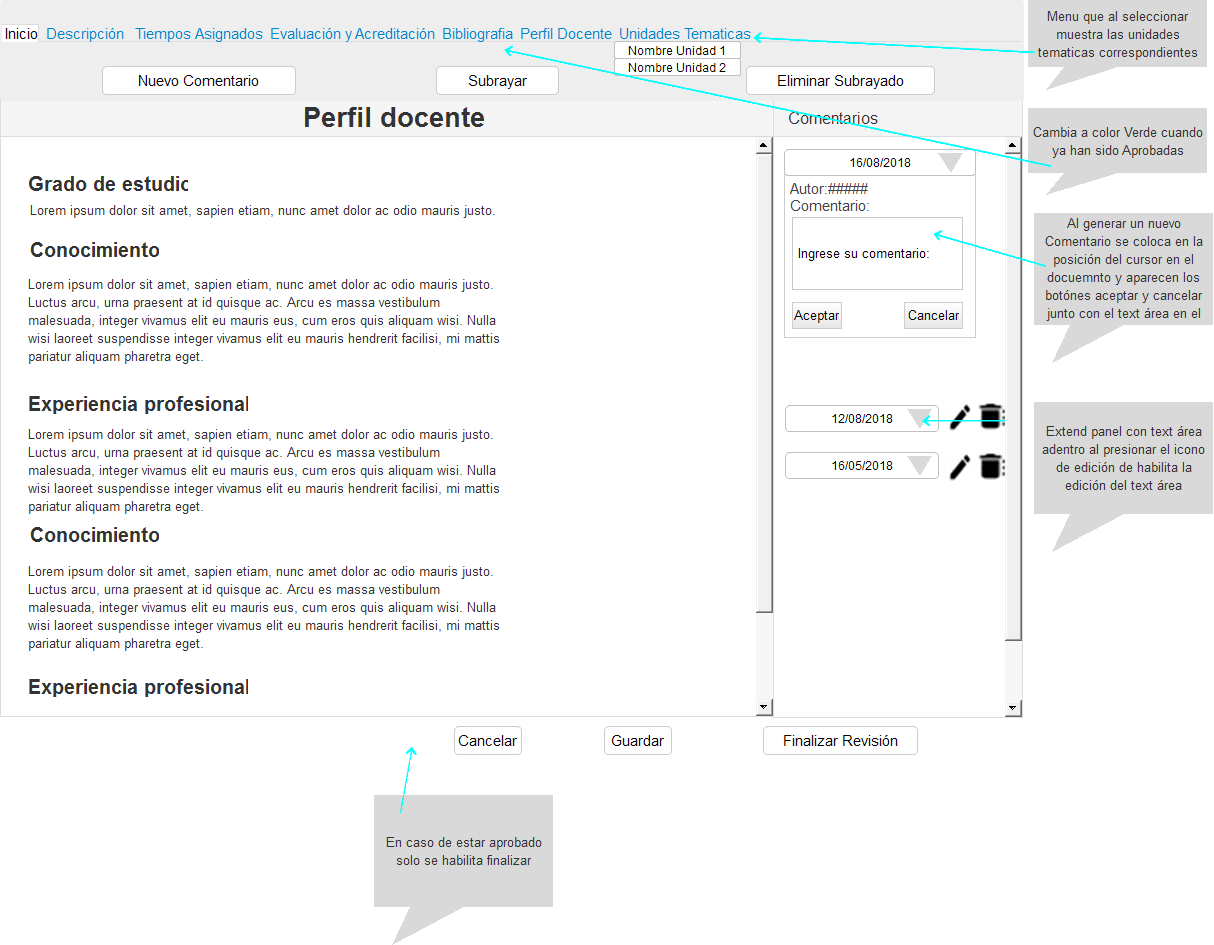
\includegraphics[width=0.7\textwidth]{DCU/SP2/Pantallas/Nuevo_comentario}
  \caption{SP2-IU-Nuevo comentario}
  \label{SP2-IU-Nuevo_comentario}
\end{figure}

\chapter{SP2-CU17 Agregar subrayado a propuesta de unidad de aprendizaje}
\begin{UseCase}{SP2-CU17}{ Agregar subrayado a propuesta de unidad de aprendizaje }{El usuario podrá agregar uno o más subrayados al texto a la sección de propuesta de unidad de aprendizaje que está revisando.}
		\UCitem{Versión}{\color{Gray}1.0}
		\UCitem{Autor}{\color{Gray}Romero Ponce Mauricio Isaac}
		\UCitem{Supervisa}{\color{Gray}Parra Garcilazo Cinthya Dolores}
		\UCitem{Actor}{Analista}
		\UCitem{Propósito}{Asignar puntos importantes a revisar por medio de subrayados en la propuesta de unidad de aprendizaje.}
		\UCitem{Entradas}{Las dos entradas para agregar un subrayado en una sección de la propuesta de unidad de aprendizaje son:
          \begin{itemize}
          	\item Posición en la que se agregará el subrayado.
          	\item Texto que se subraya.
           % \item fecha en que se genera el nuevo comentario.
            %\item Identificador unico del analista.
          \end{itemize}
        }
		\UCitem{Origen}{Mouse}
		\UCitem{Salidas}{
        	\begin{itemize}
        		\hypertarget{MSG12}{\item MSG12. Error: Primero se debe seleccionar el punto en donde se agregará el subrayado.}
        	\end{itemize}
        }
		\UCitem{Destino}{Pantalla.}
		\UCitem{Precondiciones}{ Se llamó el caso de uso SP2-CU7 o SP2-CU8 o SP2-CU9 o SP2-CU10 o  SP2-CU11 o SP2-CU12}
		\UCitem{Postcondiciones}{
            \begin{itemize}
                \item Se agregará al sistema el subrayado
                \item Se mostrará en el documento el subrayado en amarillo.
                \item Se habilita la llamada al caso de uso SP2-CU18  
             \end{itemize}  
        }
		\UCitem{Errores}{}
		\UCitem{Estado}{Revisión.}
		\UCitem{Observaciones}{}
\end{UseCase}

%--------------------------- CU TRAYECTORIA PRINCIPAL -------------------------
\begin{UCtrayectoria}{Principal}

    \UCpaso[\UCactor] Selecciona con el mouse el texto donde pondrá un subrayado de texto.

    \UCpaso[\UCactor] Presiona el botón \IUbutton{Subrayar}. \hyperref[SP2-CU17-A]{Trayectoria A}. 
    
    \UCpaso Verifica que se haya subrayado una sección del texto. 
    
    \UCpaso A la sección del texto seleccionada se le agrega un color de resaltado de textos de color amarillo.

\end{UCtrayectoria}

%------------------------ CU TRAYECTORIA ALTERNARIVA A -------------------------
\label{SP2-CU17-A}
\begin{UCtrayectoriaA}{A}{El usuario no seleccionó alguna parte del texto.}

	\UCpaso El sistema detecta que no hay referencia en el texto para el subrayado.

  \UCpaso El sistema muestra el \MSGref{MSG12}{Error: Primero se debe seleccionar el punto en donde se agregará el subrayado}.

  \UCpaso[\UCactor] Cierra el mensaje presionando \IUbutton{Aceptar}.

  \UCpaso continúa en el paso 1 de la trayectoria principal del CU-V14.
\end{UCtrayectoriaA}

\chapter{Pantallas}
 \begin{figure}
  \centering
    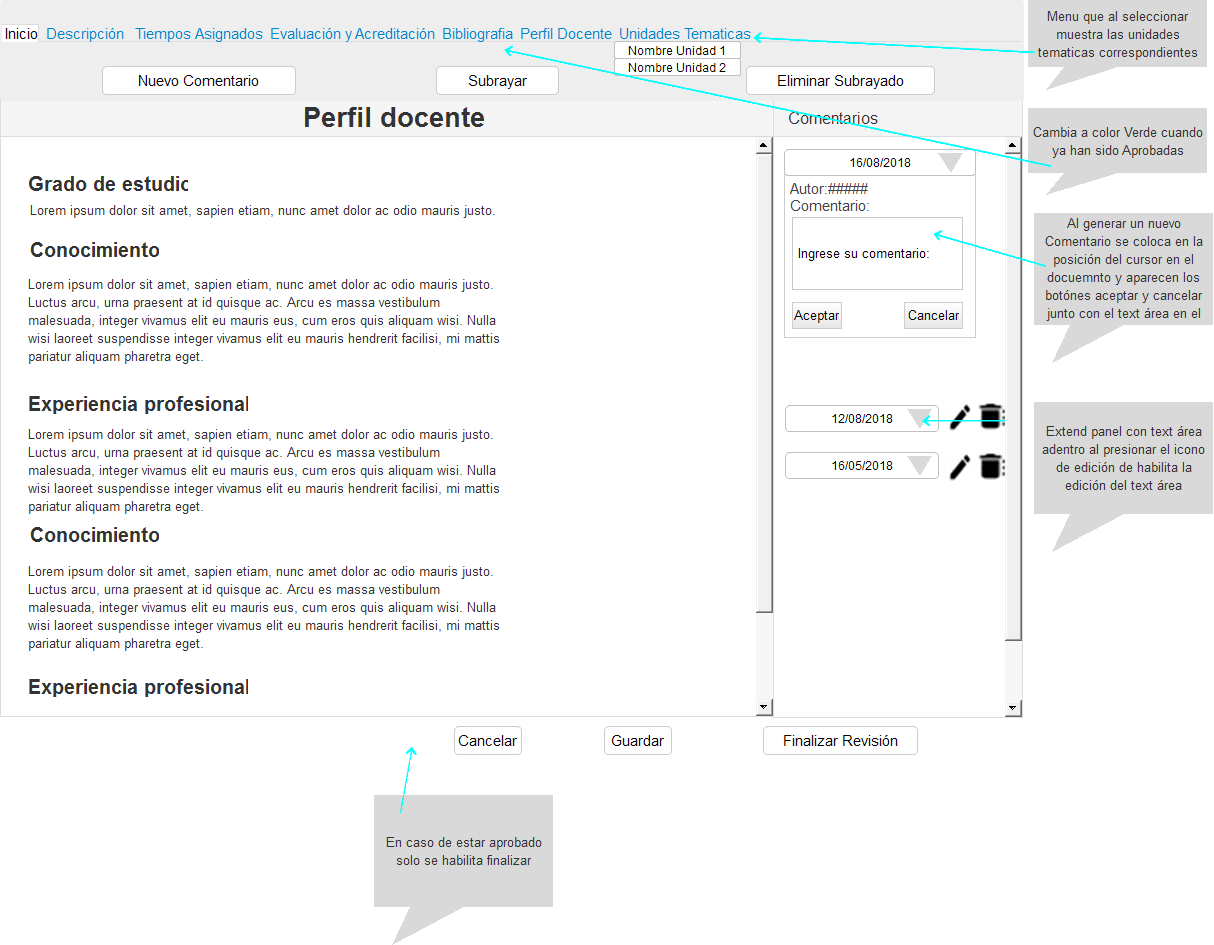
\includegraphics[width=0.7\textwidth]{DCU/SP2/Pantallas/Nuevo_comentario}
  \caption{SP2-IU-Nuevo comentario}
  \label{SP2-IU-Nuevo_comentario}
\end{figure}

% 

\begin{UseCase}{SP2-CU3}{Desasignar unidades de aprendizaje a un analista}{El usuario jefe de desarrollo e innovación curricular podrá modificar a los analistas encargados de una unidad de aprendizaje.}
		\UCitem{Versión}{\color{Gray}1.0}
		\UCitem{Autor}{\color{Gray}Parra Garcilazo Cinthya Dolores}
		\UCitem{Supervisa}{\color{Gray}}
		\UCitem{Actor}{\hyperlink{Usuario}{Jefe de Desarrollo e Innovación Curricular}}
		\UCitem{Propósito}{Asignar el acceso a una unidad de aprendizaje a otro analista.}
		\UCitem{Entradas}{Las entradas para modificar una unidad de aprendizaje a otro analista son:
          \begin{itemize}
          	\item Analista
          \end{itemize}
        }
		\UCitem{Origen}{Teclado, mouse.}
		\UCitem{Salidas}{
        	\begin{itemize}
        	   \item MSG31. Los cambios se guardaron exitosamente.
        	\end{itemize}
        }
		\UCitem{Destino}{Pantalla.}
		\UCitem{Precondiciones}{ Debe haber una analista ya asignado a esa revisión.}
		\UCitem{Postcondiciones}{El nuevo analista asignado puede acceder a la propuesta de unidad de aprendizaje y realizar los comentarios pertinentes. El analista previo no puede acceder a la información.}
		\UCitem{Errores}{}
		\UCitem{Estado}{Revisión.}
		\UCitem{Observaciones}{}
\end{UseCase}

%--------------------------- CU TRAYECTORIA PRINCIPAL -------------------------
\begin{UCtrayectoria}{Principal}


    \UCpaso Muestra la interfaz de usuario \IUref{GestionEncargado}
    \UCpaso [\UCactor] Presiona el botón \IUbutton {Editar}
    \UCpaso Activa los campos de fecha y analista.
    \UCpaso [\UCactor] Selecciona el campo de analista.
    \UCpaso Despliega la lista de analistas registrados en la base de datos.
    \UCpaso[\UCactor] Selecciona una opcion.
    \UCpaso [\UCactor] Presiona el botón \IUbutton {Confirmar}
    \UCpaso Modifica en la base de datos al analista asignado para la revisión de la unidad de aprendizaje.
    \UCpaso Muestra el mensaje \MSGref {MSG31}{Los cambios se guardaron exitosamente.}
    \UCpaso[\UCactor] Presiona el botón \IUbutton {Aceptar}

\end{UCtrayectoria}

% \chapter{SP2-CU4 Desasignar unidades de aprendizaje a un analista }

\begin{UseCase}{SP2-CU4}{Desasignar unidades de aprendizaje a un analista}{El usuario jefe de desarrollo e innovación curricular podrá modificar a los analistas encargados de una unidad de aprendizaje.}
		\UCitem{Versión}{\color{Gray}1.0}
		\UCitem{Autor}{\color{Gray}Parra Garcilazo Cinthya Dolores}
		\UCitem{Supervisa}{\color{Gray}}
		\UCitem{Actor}{\hyperlink{Usuario}{Jefe de Desarrollo e Innovación Curricular}}
		\UCitem{Propósito}{Asignar el acceso a una unidad de aprendizaje a otro analista.}
		\UCitem{Entradas}{Las entradas para modificar una unidad de aprendizaje a otro analista son:
          \begin{itemize}
          	\item Analista
          \end{itemize}
        }
		\UCitem{Origen}{Teclado, mouse.}
		\UCitem{Salidas}{
        	\begin{itemize}
        	   \item MSG31. Los cambios se guardaron exitosamente.
        	\end{itemize}
        }
		\UCitem{Destino}{Pantalla.}
		\UCitem{Precondiciones}{ Debe haber una analista ya asignado a esa revisión.}
		\UCitem{Postcondiciones}{El nuevo analista asignado puede acceder a la propuesta de unidad de aprendizaje y realizar los comentarios pertinentes. El analista previo no puede acceder a la información.}
		\UCitem{Errores}{}
		\UCitem{Estado}{Revisión.}
		\UCitem{Observaciones}{}
\end{UseCase}

%--------------------------- CU TRAYECTORIA PRINCIPAL -------------------------
\begin{UCtrayectoria}{Principal}


    \UCpaso Muestra la interfaz de usuario \IUref{GestionEncargado}
    \UCpaso [\UCactor] Presiona el botón \IUbutton {Editar}
    \UCpaso Activa los campos de fecha y analista.
    \UCpaso [\UCactor] Selecciona el campo de analista.
    \UCpaso Despliega la lista de analistas registrados en la base de datos.
    \UCpaso[\UCactor] Selecciona una opcion.
    \UCpaso [\UCactor] Presiona el botón \IUbutton {Confirmar}
    \UCpaso Modifica en la base de datos al analista asignado para la revisión de la unidad de aprendizaje.
    \UCpaso Muestra el mensaje \MSGref {MSG31}{Los cambios se guardaron exitosamente.}
    \UCpaso[\UCactor] Presiona el botón \IUbutton {Aceptar}

\end{UCtrayectoria}



%------------------------ Pantallas de este caso de uso -------------------------
\chapter{Pantallas}
 \begin{figure}
  \centering
    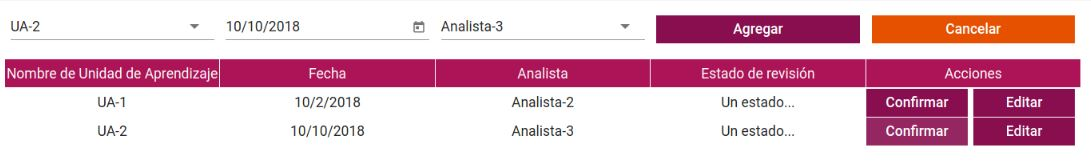
\includegraphics[width=0.7\textwidth]{DCU/SP2/Pantallas/GestionEncargado}
  \caption{SP2-IU-GestionEncargado}
  \label{SP2-IU-GestionEncargado}
\end{figure}

% \chapter{SP2-CU7 Finalizar revisión de paquetes de propuestas de unidades de aprendizaje}

\begin{UseCase}{SP2-CU5}{Finalizar revisión de paquetes de propuestas de unidades de aprendizaje}{El usuario jefe de desarrollo e innovación curricular podrá aprobar un paquete de unidades de aprendizaje.}
		\UCitem{Versión}{\color{Gray}1.0}
		\UCitem{Autor}{\color{Gray}Parra Garcilazo Cinthya Dolores}
		\UCitem{Supervisa}{\color{Gray}}
		\UCitem{Actor}{\hyperlink{Usuario}{Jefe de Desarrollo e Innovación Curricular}}
		\UCitem{Propósito}{Dar por concluida la revisón de un paquete de Unidades de Aprendizaje.}
		\UCitem{Entradas}{Las entradas para el registro de una referencia bibliográfica serán:
          \begin{itemize}
          	\item Unidades de aprendizaje
          	\item Unidad Académica
            \item Semestre
            \item Analistas
          \end{itemize}
        }
		\UCitem{Origen}{Teclado, mouse.}
		\UCitem{Salidas}{
        	\begin{itemize}
        	   \item MSG. Revisión de paquete finalizada. Paquete enviado.
                \item MSG2. Error al finalizar paquete.

        	\end{itemize}
        }
		\UCitem{Destino}{Pantalla.}
		\UCitem{Precondiciones}{ Se sigue la SP2-BR10.}
		\UCitem{Postcondiciones}{El paquete es enviado a la unidad de aprendizaje correspondiete como aprobado, no se hacen más modificaciones a ninguna unidad de aprendizaje.}
		\UCitem{Errores}{}
		\UCitem{Estado}{Revisión.}
		\UCitem{Observaciones}{}
\end{UseCase}

%--------------------------- CU TRAYECTORIA PRINCIPAL -------------------------
\begin{UCtrayectoria}{Principal}


    \UCpaso Muestra la interfaz de usuario \IUref{SP2-IU-GestionPaquetes}
    \UCpaso[\UCactor] Presiona el botón \IUbutton {Finalizar}
    \UCpaso Verifica en la base de datos que todas las unidades de aprendizaje tengan el estado de revisado\hyperref[SP2-CU5-A]{Trayectoria A}.
    \UCpaso Envía notificación a la Unidad de Aprendizaje correspondiente de Paquete Aprobado. \hyperref[SP2-CU5-B]{Trayectoria B}.
    \UCpaso Muestra el mensaje \MSGref {MSG1}
    \UCpaso[\UCactor] Presiona el botón \IUbutton {Aceptar}
    \UCpaso Cambia el estado del paquete a enviado.
    \UCpaso Remueve la tabla con la información del paquete aprobado de la lista de tareas.

\end{UCtrayectoria}


%------------------------ CU TRAYECTORIA ALTERNARIVA A -------------------------
\label{SP2-CU5-A}
\begin{UCtrayectoriaA}{A}{No están todas las unidades de aprendizaje en estado de aprobado.}
    \UCpaso Muestra el mensaje \MSGref {MSG6}
    \UCpaso[\UCactor] Presiona el botón \IUbutton {Aceptar}
\end{UCtrayectoriaA}

%------------------------ CU TRAYECTORIA ALTERNARIVA B -------------------------

\label{SP2-CU5-B}
\begin{UCtrayectoriaA}{B}{No están todas las unidades de aprendizaje en estado de aprobado.}
    \UCpaso Muestra el mensaje \MSGref {MSG5}
    \UCpaso[\UCactor] Presiona el botón \IUbutton {Aceptar}
\end{UCtrayectoriaA}


%------------------------ Pantallas de este caso de uso -------------------------
\chapter{Pantallas}
 \begin{figure}
  \centering
    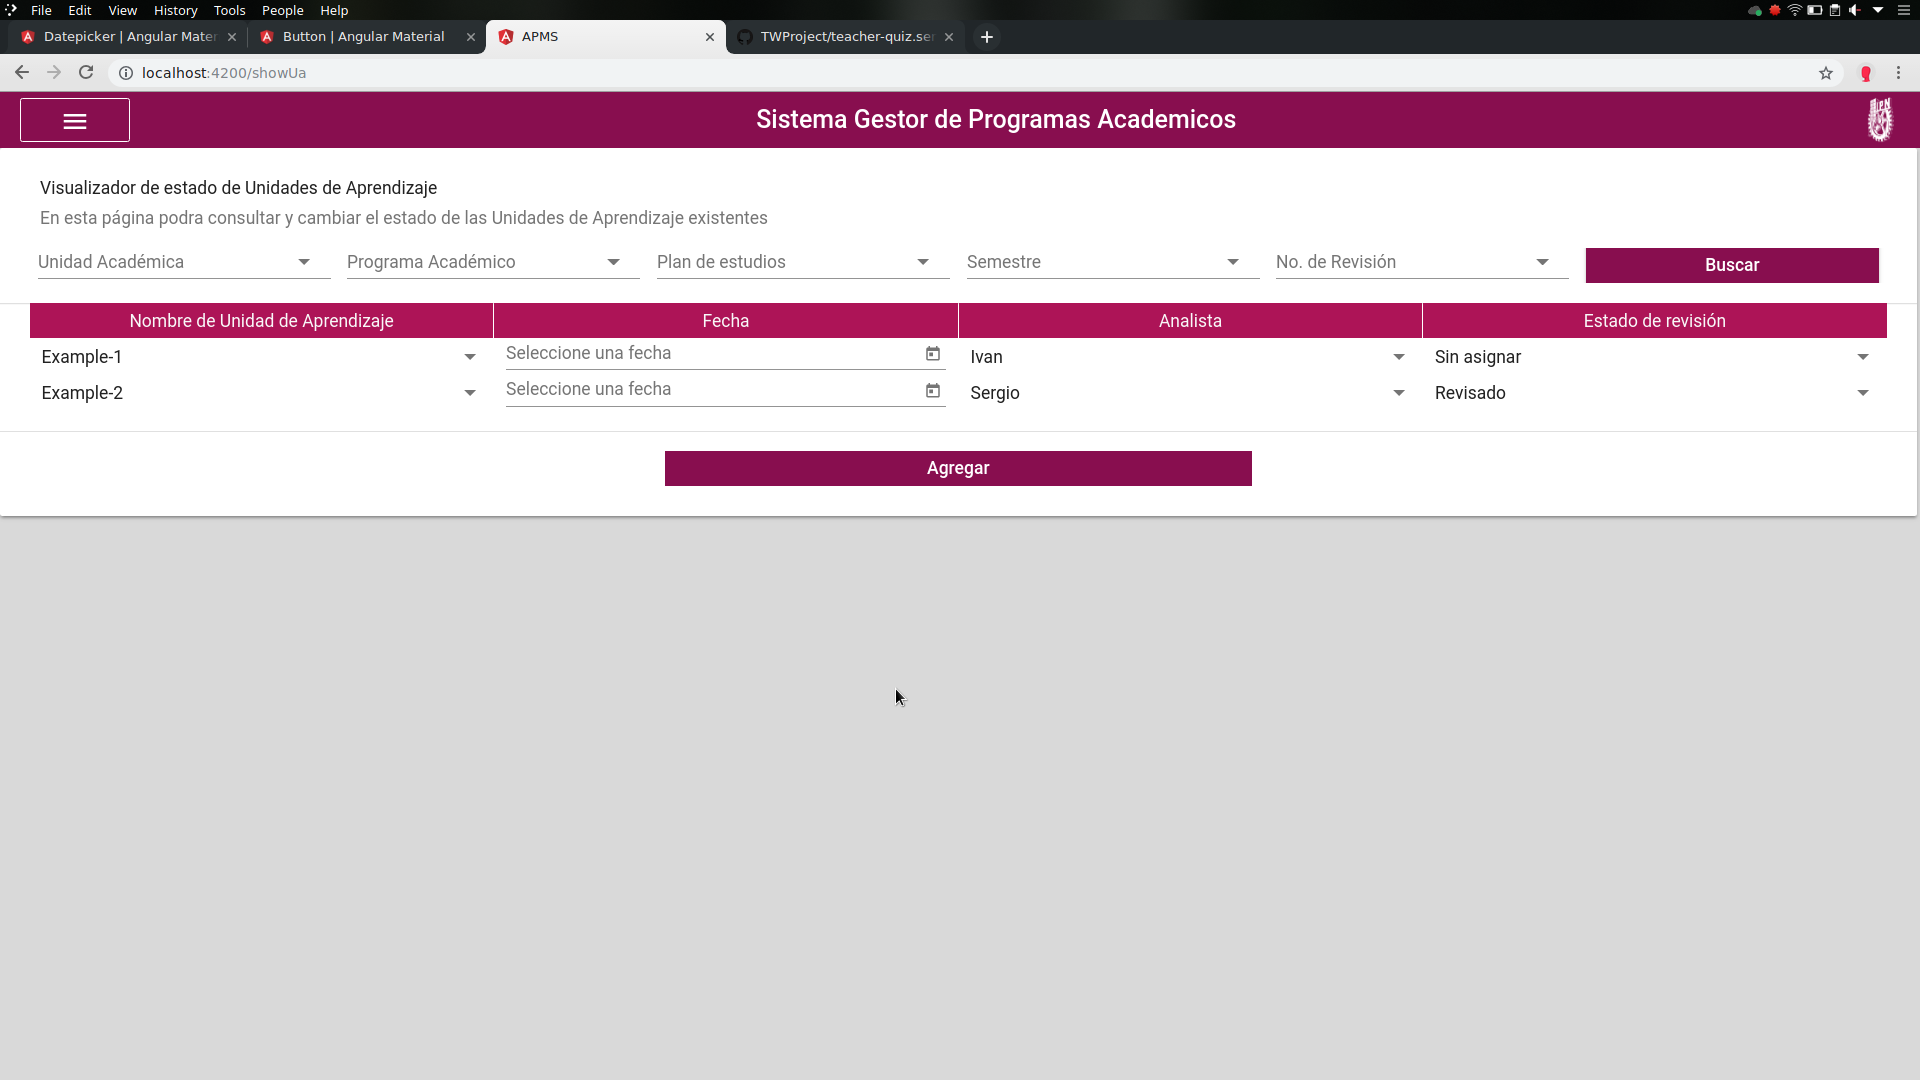
\includegraphics[width=0.7\textwidth]{DCU/SP2/Pantallas/GestionPaquetes}
  \caption{SP2-IU-GestionPaquetes}
  \label{SP2-IU-GestionPaquetes}
\end{figure}

%------------------------ Mensajes de este caso de uso -------------------------
\chapter{Pantallas}
 \begin{figure}
  \centering
    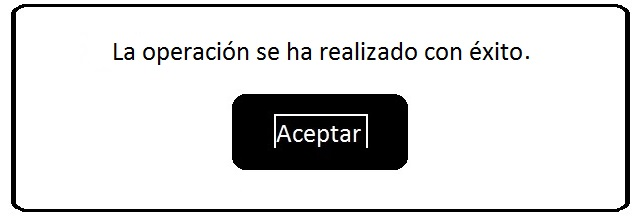
\includegraphics[width=0.7\textwidth]{DCU/SP2/mensajes/MSG1}
   \caption{SP2-MSG1}
  \label{SP2-MSG1}
\end{figure}

 \begin{figure}
  \centering
    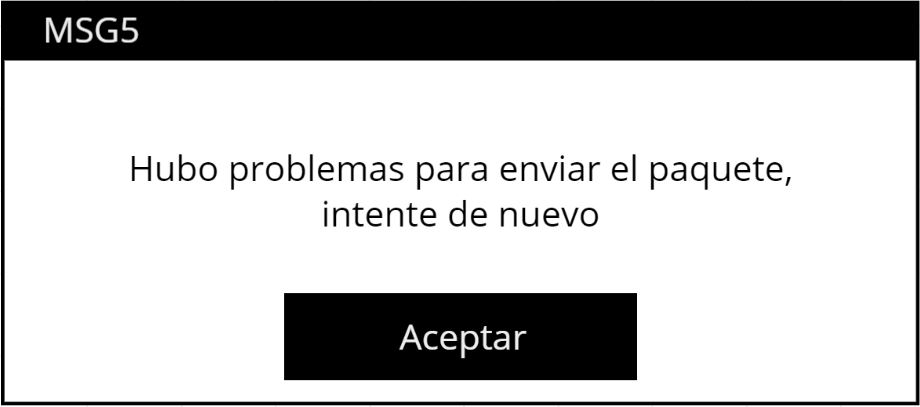
\includegraphics[width=0.7\textwidth]{DCU/SP2/mensajes/MSG5}
  \caption{SP2-MSG5}
  \label{SP2-MSG5}
\end{figure}

 \begin{figure}
  \centering
    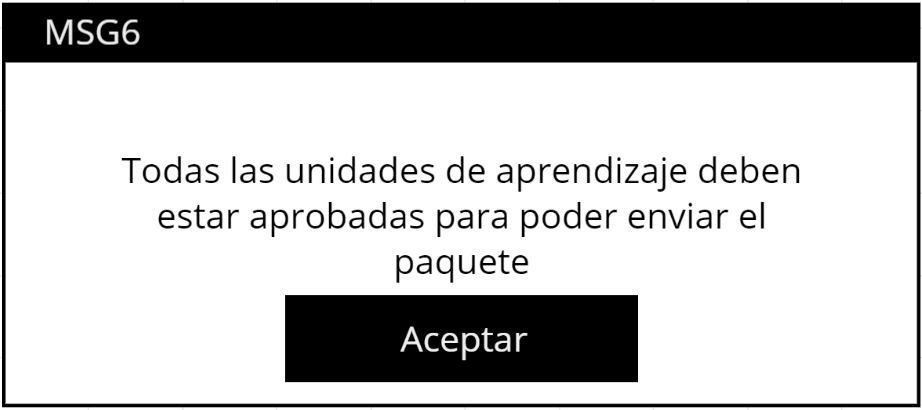
\includegraphics[width=0.7\textwidth]{DCU/SP2/mensajes/MSG6}
  \caption{SP2-MSG6}
  \label{SP2-MSG6}
\end{figure}


% REGISTRAR BIBLIOGRAFÍA.
\begin{UseCase}{SP4-CU1}{Registrar Programa Académico}{El usuario Jefe de Innovación Educativa ingresa los datos de un Programa Académico.}
		\UCitem{Versión}{\color{Gray}1.0}
		\UCitem{Autor}{\color{Gray}Plata García Josué Eliasaf}
		\UCitem{Supervisa}{\color{Gray}}
		\UCitem{Actor}{\hyperlink{Usuario}{Jefe de Innovación Educativa}}
		\UCitem{Propósito}{Registrar el nombre del Programa Académico en el sistema.}
		\UCitem{Entradas}{Las entradas para el registro de Programa Académico:
          \begin{itemize}
          	\item Nombre (Tipo Alfanumérico)
          \end{itemize}
        }
		\UCitem{Origen}{Teclado.}
		\UCitem{Salidas}{
        	\begin{itemize}
        		\item \MSGref{MSG32}{Todos los campos son obligatorios}
                \item \MSGref{MSG5}{Registro finalizado exitosamente.}
                \item \MSGref{MSG29}{¿Está seguro que desea cancelar? Se perderán todos los avances sin guardar.}
                \item \MSGref{MSG20}{Los campos no fueron contestados correctamente.}
        	\end{itemize}
        }
		\UCitem{Destino}{Pantalla.}
		\UCitem{Precondiciones}{}
		\UCitem{Postcondiciones}{El Programa Académico quedó registrado en el sistema, permitiendo consultarlo y generar tareas de registro del mismo.}
		\UCitem{Errores}{E1. El nombre del Programa Académico contiene uno o más caracteres no alfanuméricos.}
		\UCitem{Estado}{Revisión.}
		\UCitem{Observaciones}{El nombre de un Programa Académico puede ser igual a otro.}
\end{UseCase}

%--------------------------- CU TRAYECTORIA PRINCIPAL -------------------------
\begin{UCtrayectoria}{Principal}

    \UCpaso[\UCactor] Presiona el botón \IUbutton{Registrar Programa Académico} de la interfaz de usuario \IUref{IU2.2-J}{Consultar Programas Académicos}

    \UCpaso Muestra la interfaz de usuario \IUref{IU2.2.1-J}{Registrar Programa Académico}.
    \UCpaso[\UCactor] Ingresa el nombre del Programa Académico.

    \UCpaso[\UCactor] Termina la operación presionando el botón \IUbutton{Guardar}. [Trayectoria A] [Trayectoria B]

    \UCpaso Verifica que todos los campos marcados como obligatorios hayan sido contestados. [Trayectoria C][Trayectoria D]

    \UCpaso Guarda la información del Programa Académico correspondiente.

    \UCpaso El sistema muestra el mensaje \MSGref{MSG5}{Registro finalizado exitosamente}.

    \UCpaso[\UCactor] Cierra el mensaje presionando el botón \IUbutton{Aceptar}.

    \UCpaso Muestra la interfaz de usuario \IUref{IU2.2-J}{Consultar Programas Académicos}.
\end{UCtrayectoria}


%------------------------ CU TRAYECTORIA ALTERNARIVA A -------------------------


\begin{UCtrayectoriaA}{A}{El actor quiere cancelar el registro de la bibliografía.}
	\UCpaso[\UCactor] Presiona el botón \IUbutton{Cancelar}.
    \UCpaso Muestra el mensaje \MSGref{MSG3}{¿Seguro que desea cancelar el registro?}.
    \UCpaso[\UCactor] Confirma la operación presionando el botón \IUbutton{Si}.
    \UCpaso Muestra la interfaz de usuario \IUref{IU2.2-J}{Consultar Programas Académicos}
\end{UCtrayectoriaA}


%------------------------ CU TRAYECTORIA ALTERNARIVA B -------------------------

\begin{UCtrayectoriaA}{B}{El actor presiona accidentalmente el botón Cancelar}
	\UCpaso[\UCactor] Presiona el botón \IUbutton{Cancelar}
    \UCpaso Muestra el mensaje \MSGref{MSG29}{¿Está seguro que desea cancelar? Se perderán todos los avances sin guardar.}.
    \UCpaso[\UCactor] Presiona el botón \IUbutton{No}.
    \UCpaso Cierra el mensaje.
    \UCpaso Continúa en el paso 4 de la trayectoria principal del \UCref{SP4-CU1}.
\end{UCtrayectoriaA}

%------------------------ CU TRAYECTORIA ALTERNARIVA C -------------------------

\begin{UCtrayectoriaA}{C}{Uno o más campos obligatorios no fueron contestados.}
	\UCpaso Detecta uno o más campos sin contestar.
    \UCpaso Muestra el mensaje \MSGref{MSG32}{Todos los campos son obligatorios}.
    \UCpaso[\UCactor] Cierra el mensaje presionando el botón \IUbutton{Aceptar}.
    \UCpaso Continúa en el paso 3 de la trayectoria principal del \UCref{SP4-CU1}.
\end{UCtrayectoriaA}
%------------------------ CU TRAYECTORIA ALTERNARIVA D -------------------------

\begin{UCtrayectoriaA}{D}{El Nombre de Programa Académico contiene caracteres no alfanuméricos}
	\UCpaso El Sistema detecta caracteres no alfanuméricos E1.
    \UCpaso Muestra el mensaje \MSGref{MSG20}{Los campos no fueron contestados correctamente.}.
    \UCpaso Continúa en el paso 1 de la trayectoria principal del \UCref{SP4-CU1}.
\end{UCtrayectoriaA}


% REGISTRAR PLAN DE ESTUDIOS.
\begin{UseCase}{SP4-CU2}{Registrar Plan de Estudios}{El usuario Jefe de Innovación ingresa los datos del Plan de Estudios, acorde a la entidad Plan de Estudios del Modelo de Datos.}
		\UCitem{Versión}{\color{Gray}3.0}
		\UCitem{Autor}{\color{Gray}Cervantes Moreno Christian Andres}
		\UCitem{Supervisa}{\color{Gray} Evelyn Reyes}
		\UCitem{Actor}{\hyperlink{Usuario}{Jefe de Innovación}}
		\UCitem{Propósito}{Registrar el año, modalidad, total de créditos (TEPIC / SATCA) y horas totales (Prácticas / Teóricas) a un Plan de Estudios.}
		\UCitem{Entradas}{Las entradas para el registro del Plan de Estudios serán:
          \begin{itemize}
          	\item Año.
          	\item Créditos Totales TEPIC.
            \item Créditos Totales SATCA.
            \item Total horas / Teoría.
            \item Total horas / Práctica.
            \item Modalidad.
          \end{itemize}
        }
		\UCitem{Origen}{Teclado, Mouse}
		\UCitem{Salidas}{
        	\begin{itemize}

                \item \MSGref{MSG5}{Registro finalizado exitosamente.}
                \item \MSGref{MSG29}{ ¿Está seguro que desea cancelar? Se perderán todos los avances sin guardar.}
                \item \MSGref{MSG35}{Escribe información válida}
               \item \MSGref{MSG44}{Este campo es requerido}
                \item \MSGref{MSG7}{ Los catálogos necesarios no se han cargado, favor de intentarlo más tarde. }
                \item \MSGref{MSG25}{Servicios no disponibles por el momento.}
                \item \MSGref{MSG46}{Las horas totales de teoría y práctica deben de estar en el rango 350 y 450.}
        	\end{itemize}
        }
		\UCitem{Destino}{Pantalla.}
		\UCitem{Precondiciones}{Debe de existir al menos un Programa Académico en el sistema.}
		\UCitem{Postcondiciones}{El Plan de Estudios queda registrado en el sistema.}
		\UCitem{Errores}{
			  \begin{itemize}
				\item E1. El catálogo de modalidad no se cargaro correctamente.
				\item E2. Hubo un problema al conectarse con la base de datos.
			\end{itemize}
		}
		\UCitem{Estado}{Revisión.}
		\UCitem{Observaciones}{}
\end{UseCase}
%--------------------------- CU TRAYECTORIA PRINCIPAL -------------------------
\begin{UCtrayectoria}{Principal}
    %Usuario
    \UCpaso[\UCactor] Presiona el boton \IUbutton{+} que se encuentra de la interfaz de usuario \IUref{GPE-J}{Gestionar Planes de Estudio}
	%Sistema
    \UCpaso Carga el catálogo de modalidad descrito en la \BRref{BR14}{Existen los catálogos}.[Trayectoria A]
    \UCpaso Muestra la interfaz de usuario \IUref{RPE-J}{Registrar Plan de Estudios}.
    \UCpaso[\UCactor] Ingresa el año del Plan de Estudios.
    \UCpaso[\UCactor] Selecciona la modalidad del Plan de Estudios.
    \UCpaso[\UCactor] Ingresa los créditos totales TEPIC del Plan de Estudios.
    \UCpaso[\UCactor] Ingresa los créditos totales SATCA del Plan de Estudios.
    \UCpaso[\UCactor] Ingresa Total horas / Teoría del Plan de Estudios considerando \BRref{BR20}{Las horas totales deben de estar entre 350 y 450 horas}.
    \UCpaso[\UCactor] Ingresa Total horas / Práctica del Plan de Estudios  considerando \BRref{BR20}{Las horas totales deben de estar entre 350 y 450 horas}.
    \UCpaso[\UCactor] Termina la operación presionando el botón \IUbutton{Registrar}. [Trayectoria B] [Trayectoria B.1]
    \UCpaso Verifica que se cumpla la \BRref{BR33}{Información de Planes de Estudios}. [Trayectoria C] [Trayectoria D] [Trayectoria F]
    \UCpaso Persiste los datos ingresados. [Trayectoria E]
    \UCpaso El sistema muestra el mensaje \MSGref{MSG5}{Registro finalizado exitosamente}.
    \UCpaso[\UCactor] Cierra el mensaje presionando el botón \IUbutton{Aceptar}.
    \UCpaso Muestra la interfaz de usuario \IUref{GPE-J}{Gestionar Planes de Estudios}.
\end{UCtrayectoria}
%------------------------ CU TRAYECTORIA ALTERNARIVA A -------------------------
\begin{UCtrayectoriaA}{A}{ Los catálogos de la \BRref{BR14}{Existen los catálogos} necesarios no se pudieron cargar.}
	\UCpaso Muestra el mensaje \MSGref{MSG7}{ Los catálogos necesarios no se han cargado, favor de intentarlo más tarde. }
	\UCpaso[\UCactor] Cierra el mensaje presionando el botón \IUbutton{Aceptar}.
\end{UCtrayectoriaA}

%------------------------ CU TRAYECTORIA ALTERNARIVA B -------------------------
\begin{UCtrayectoriaA}{B}{El actor presiona el botón \IUbutton{Cancelar}.}
	\UCpaso Muestra el mensaje \MSGref{MSG29}{¿Está seguro que desea cancelar? Se perderán todos los avances sin guardar}.
	\UCpaso[\UCactor] Confirma la operación presionando el botón \IUbutton{Si}.
	\UCpaso Muestra la interfaz de usuario \IUref{GPE-J}{Gestionar Planes de Estudio}
\end{UCtrayectoriaA}

%------------------------ CU TRAYECTORIA ALTERNARIVA B.1 -------------------------
\begin{UCtrayectoriaA}{B.1}{El actor presiona accidentalmente el botón \IUbutton{Cancelar}.}
	\UCpaso[\UCactor] Presiona el botón \IUbutton{Cancelar}
	\UCpaso Muestra el mensaje \MSGref{MSG29}{¿Está seguro que desea cancelar? Se perderán todos los avances sin guardar}.
	\UCpaso[\UCactor] Presiona el botón \IUbutton{No}.
	\UCpaso Cierra el mensaje.
	\UCpaso Continúa en el paso 4 de la trayectoria principal del \UCref{SP4-CU2}.
\end{UCtrayectoriaA}

%------------------------ CU TRAYECTORIA ALTERNARIVA C -------------------------
\begin{UCtrayectoriaA}{C}{El sistema detecta uno o más campos sin contestar incumpliendo con la \BRref{BR33}{Información de Planes de Estudios}.}
	\UCpaso Muestra el mensaje \MSGref{MSG44}{debajo de cada campo obligatorio sin contestar}.
	\UCpaso Continúa en el paso 4 de la trayectoria principal del \UCref{SP4-CU2}.
\end{UCtrayectoriaA}

%------------------------ CU TRAYECTORIA ALTERNARIVA D -------------------------
\begin{UCtrayectoriaA}{D}{El sistema detecta caracteres no numéricos.}
	\UCpaso Muestra el mensaje \MSGref{MSG35}{Escribe información válida} debajo del campo que incumplio la \BRref{BR33}{Información de Planes de Estudios}.
	\UCpaso Continúa en el paso 4 de la trayectoria principal del \UCref{SP4-CU2}.
\end{UCtrayectoriaA}

%------------------------ CU TRAYECTORIA ALTERNARIVA E -------------------------
\begin{UCtrayectoriaA}{E}{Ocurre un error al momento de persistir los datos.}
	\UCpaso Muestra el mensaje \MSGref{MSG25}{Servicios no disponibles por el momento}.
    \UCpaso[\UCactor] Cierra el mensaje presionando el botón \IUbutton{Aceptar}.
	\UCpaso Muestra la interfaz de usuario \IUref{RPE-J}{Registrar Plan de Estudios}.
\end{UCtrayectoriaA}


%------------------------ CU TRAYECTORIA ALTERNARIVA F -------------------------
\begin{UCtrayectoriaA}{F}{El sistema detecta incumplimiento de la \BRref{BR20}{Las horas totales deben de estar entre 350 y 450 horas}.}
	\UCpaso Muestra el mensaje \MSGref{MSG46}{Las horas totales de teoría y práctica deben de estar en el rango 350 y 450.} debajo del campo que incumplio la \BRref{BR20}{Las horas totales deben de estar entre 350 y 450 horas}..
	\UCpaso Continúa en el paso 4 de la trayectoria principal del \UCref{SP4-CU2}.
\end{UCtrayectoriaA}
% REGISTRAR UNIDAD DE APRENDIZAJE.
\begin{UseCase}{SP4-CU3}{Registrar Unidad de Aprendizaje}{El usuario Jefe de Innovación registra los datos de las Unidades de Aprendizaje del Modelo de Datos, que contiene el Mapa Curricular.}
		\UCitem{Versión}{\color{Gray}1.0}
		\UCitem{Autor}{\color{Gray}Cervantes Moreno Christian Andres}
		\UCitem{Supervisa}{\color{Gray} Evelyn Reyes}
		\UCitem{Actor}{\hyperlink{Usuario}{Jefe de Innovación}}
		\UCitem{Propósito}{Registrar el nombre, créditos TEPIC, créditos SATCA, horas Teoría/Semana, horas Práctica/semana, Área de formación y semestre de una Unidad de Aprendizaje.}
		\UCitem{Entradas}{Las entradas para el registro de la Unidad de Aprendizaje serán:
          \begin{itemize}
          	\item Nombre.
          	\item Créditos TEPIC.
            \item Créditos SATCA.
            \item  Horas Teoría/Semana
            \item  Horas Práctica/Semana
            \item Área de Formación.
            \item Semestre
          \end{itemize}
        }
		\UCitem{Origen}{Teclado, Mouse}
		\UCitem{Salidas}{
        	\begin{itemize}
                \item \MSGref{MSG32}{Todos los campos son obligatorios.}
                \item \MSGref{MSG5}{Registro finalizado exitosamente.}
                \item \MSGref{MSG29}{¿Está seguro que desea cancelar? Se perderán todos los avances sin guardar.}
                \item \MSGref{MSG7}{Los catálogos necesarios no se han cargado, favor de intentarlo más tarde.}
                \item \MSGref{MSG35}{Inconsistencia en los datos. Verifique los campos e intente de nuevo.}
                \item \MSGref{MSG25}{Servicios no disponibles por el momento.}
        	\end{itemize}
        }
		\UCitem{Destino}{Pantalla.}
		\UCitem{Precondiciones}{ Debe de existir al menos un Plan de Estudios en el sistema.}
		\UCitem{Postcondiciones}{La Unidad de Aprendizaje queda registrada en el sistema.}
		\UCitem{Errores}{
			  \begin{itemize}
				\item E1. Los catálogos de tipo de usuario no se cargaron correctamente.
				\item E2. Hubo un problema al conectarse con la base de datos.
			\end{itemize}
		}
		\UCitem{Estado}{Revisión.}
		\UCitem{Observaciones}{}
\end{UseCase}
%--------------------------- CU TRAYECTORIA PRINCIPAL -------------------------
\begin{UCtrayectoria}{Principal}
    \UCpaso[\UCactor] Presiona el botón \IUbutton{+} de la interfaz de usuario \IUref{CMC-J}{Consultar Mapa Curricular}.
    \UCpaso El sistema verifica la existencia de registros en los catálogos: Área de formación y semestre segun la \BRref{BR14}{Existen los catálogos} .
    \UCpaso El sistema carga los catálogos: Área de formación y Semestre.[Trayectoria A]
    \UCpaso Muestra la interfaz de usuario \IUref{RUA-J}{Registrar Unidad de Aprendizaje}.
    \UCpaso[\UCactor] Ingresa el nombre de la Unidad de Aprendizaje según la \BRref{BR17}{El nombre de la Unidad Académica es único} y la \BRref{BR18}{Longitud Maxima de Unidad de Aprendizaje}.
    \UCpaso[\UCactor] Captura la información necesaria de la Unidad de Aprendizaje según la \BRref{BR34}{Información de la Unidad de Aprendizaje}.
    \UCpaso[\UCactor] Termina la operación presionando el botón \IUbutton{Registrar}. [Trayectoria B] [Trayectoria C]
    \UCpaso Verifica que se cumpla la \BRref{BR13}{Todos los campos son obligatorios}. [Trayectoria D]
    \UCpaso Verifica la consistencia de la información [Trayectoria F]
    \UCpaso Guarda la información de la Unidad de Aprendizaje. [Trayectoria E]
    \UCpaso El sistema muestra el mensaje \MSGref{MSG5}{Registro finalizado exitosamente}.
    \UCpaso[\UCactor] Cierra el mensaje presionando el botón \IUbutton{Aceptar}.
    \UCpaso Muestra la interfaz de usuario \IUref{CMC-J}{Consultar Mapa Curricular}.
\end{UCtrayectoria}

%------------------------ CU TRAYECTORIA ALTERNARIVA A -------------------------
\begin{UCtrayectoriaA}{A}{El sistema no carga los catálogos: Área de formación y Semestre}
	%\UCpaso[\UCactor] Presiona el botón \IUbutton{$\bigoplus$} que se encuentra a un lado del campo ``Nombre'' del formulario \IUref{IU2}{Registro de bibliografía}  [Trayectoria A.1]r}
	\UCpaso Muestra el mensaje \MSGref{MSG7}{Los catálogos necesarios no se han cargado, favor de intentarlo más tarde. }
	\UCpaso[\UCactor] Confirma la operación presionando el botón \IUbutton{Ok}.
	 \UCpaso Muestra la interfaz de usuario \IUref{CMC-J}{Consultar Mapa Curricular}
\end{UCtrayectoriaA}
%------------------------ CU TRAYECTORIA ALTERNARIVA B -------------------------
\begin{UCtrayectoriaA}{B}{El actor presiona el botón \IUbutton{Cancelar}}
	\UCpaso Muestra el mensaje \MSGref{MSG29}{¿Está seguro que desea cancelar? Se perderán todos los avances sin guardar.}.
	\UCpaso[\UCactor] Confirma la operación presionando el botón \IUbutton{Si}.
	\UCpaso Muestra la interfaz de usuario \IUref{CMC-J}{Consultar Mapa Curricular}
\end{UCtrayectoriaA}
%------------------------ CU TRAYECTORIA ALTERNARIVA C -------------------------
\begin{UCtrayectoriaA}{C}{El actor presiona accidentalmente el botón \IUbutton{Cancelar}}
	\UCpaso Muestra el mensaje \MSGref{MSG29}{¿Está seguro que desea cancelar? Se perderán todos los avances sin guardar.}.
	\UCpaso[\UCactor] Presiona el botón \IUbutton{No}.
	\UCpaso Cierra el mensaje.
	\UCpaso Continúa en el paso 6 de la trayectoria principal del \UCref{SP4-CU3}.
\end{UCtrayectoriaA}
%------------------------ CU TRAYECTORIA ALTERNARIVA D -------------------------
\begin{UCtrayectoriaA}{D}{El sistema detecta uno o más campos sin contestar.}
	\UCpaso Muestra el mensaje \MSGref{MSG32}{Todos los campos son obligatorios.}.
	\UCpaso[\UCactor] Cierra el mensaje presionando el botón \IUbutton{Aceptar}.
	\UCpaso Continúa en el paso 6 de la trayectoria principal del \UCref{SP4-CU3}.
\end{UCtrayectoriaA}

%------------------------ CU TRAYECTORIA ALTERNARIVA E -------------------------
\begin{UCtrayectoriaA}{E}{La base de datos no está disponible, o hubo un error de conexión.}
	\UCpaso Muestra el mensaje \MSGref{MSG25}{Servicios no disponibles por el momento.}
	\UCpaso[\UCactor] Cierra el mensaje presionando el botón \IUbutton{Ok}.
	\UCpaso El sistema regresa a la interfaz de usuario\IUref{RUA-J}{Registrar Unidad de Aprendizaje}
\end{UCtrayectoriaA}

%------------------------ CU TRAYECTORIA ALTERNARIVA F -------------------------
\begin{UCtrayectoriaA}{F}{El Sistema detecta que algun campo no cumple con la expresión regular.}
	\UCpaso Muestra el mensaje \MSGref{MSG35}{Inconsistencia en los datos. Verifique los campos e intente de nuevo.}.
	\UCpaso Continúa en el paso 6 de la trayectoria principal del \UCref{SP4-CU3}.
\end{UCtrayectoriaA}
\begin{UseCase}{SP4-CU4}{Registrar Recurso Humano}{El usuario Jefe de Innovación Educativa ingresa los datos de los Recursos Humanos de su Unidad Académica.}
        \UCitem{Versión}{\color{Gray}1.1}
        \UCitem{Autor}{\color{Gray}Rivas Rojas Arturo}
        \UCitem{Supervisa}{\color{Gray}}
        \UCitem{Actor}{\hyperlink{JDIE}{Jefe de Innovación Educativa}}
        \UCitem{Propósito}{Ingresar al sistema la información necesaria de los Recursos Humanos.}
        \UCitem{Entradas}{Las entradas para el registro de un Recurso Humano serán:
          \begin{itemize}
            \item Matríacula de Empleado.
            \item Cargo.
            \item Título.
            \item Nombre.
            \item Apellido Paterno.
            \item Apellido Materno.
          \end{itemize}
        }
        \UCitem{Origen}{Teclado.}
        \UCitem{Salidas}{
            \begin{itemize}
                \item \MSGref{MSG32}{Todos los campos son obligatorios.}
                \item \MSGref{MSG5}{Registro finalizado exitosamente.}
                \item \MSGref{MSG33}{El Recurso Humano con la Matrícula de Empleado [Número de Matrícula de Empleado] ya existe.}
                \item \MSGref{MSG29}{¿Está seguro que desea cancelar? Se perderán todos los avances sin guardar.}
                \item \MSGref{MSG7}{Los catálogos necesarios no se han cargado, favor de intentarlo más tarde.}
                \item \MSGref{MSG37}{Ha ocurrido un error al guardar los datos.}
            \end{itemize}
        }
        \UCitem{Destino}{Pantalla.}
        \UCitem{Precondiciones}{
            \begin{itemize}
                \item El Recurso Humano a registrar, no debe existir previamente en el sistema.
                \item El catálogo de Cargo debe de estar cargado en el sistema.
            \end{itemize}
        }
        \UCitem{Postcondiciones}{El Recurso Humano quedará registrado en el sitema, permitiendo consultarlo y relacionarlo a una Unidad de Aprendizaje.}
        \UCitem{Errores}{
            \begin{itemize}
                \item E1. No existen o no pudieron cargarse los catálogo necesarios.
            \end{itemize}
        }
        \UCitem{Estado}{Revisión.}
        \UCitem{Observaciones}{}
\end{UseCase}
%--------------------------- CU TRAYECTORIA PRINCIPAL -------------------------
\begin{UCtrayectoria}{Principal}
    \UCpaso[\UCactor] Presiona el botón \IUbutton{(+)Registrar Recurso Humano} de la interfaz de usuario \IUref{GRH-J}{Gestionar Recursos Humanos}
    \UCpaso Carga el catálogo de Cargo descrito en la \BRref{BR14}{Catálogos existentes}. [Trayectoria A]
    \UCpaso Carga el catálogo de Título descrito en la \BRref{BR14}{Catálogos existentes}. [Trayectoria A]
    \UCpaso Muestra la interfaz de usuario \IUref{RRH-J}{Registrar Recurso Humano}.
    \UCpaso[\UCactor] Ingresa la Matrícula de Empleado.
    \UCpaso[\UCactor] Selecciona el Cargo.
    \UCpaso[\UCactor] Selecciona el Título.
    \UCpaso[\UCactor] Ingresa el Nombre.
    \UCpaso[\UCactor] Ingresa el Apellido Paterno.
    \UCpaso[\UCactor] Ingresa el Apellido Materno.
    \UCpaso[\UCactor] Termina la operación presionando el botón \IUbutton{Guardar}. [Trayectoria B] [Trayectoria B.1]
    \UCpaso Verifica que se cumpla la \BRref{BR13}{Todos los campos son obligatorios}. [Trayectoria C]
    \UCpaso Verifica que se cumpla la \BRref{BR16}{Matrícula de empleado única}. [Trayectoria D]
    \UCpaso Persiste los datos ingresados. [Trayectoria E]
    \UCpaso Muestra el mensaje \MSGref{MSG5}{Registro finalizado exitosamente}.
    \UCpaso[\UCactor] Cierra el mensaje presionando el botón \IUbutton{Aceptar}.
    \UCpaso Muestra la interfaz de usuario \IUref{GRH-J}{Gestionar Recursos Humanos}.
\end{UCtrayectoria}
%------------------------ CU TRAYECTORIA ALTERNARIVA A -------------------------
\begin{UCtrayectoriaA}{A}{Los catálogos de la \BRref{BR14}{Catálogos existentes} necesarios no se pudieron cargar.}
    \UCpaso Muestra el mensaje \MSGref{MSG7}{Los catálogos necesarios no se han cargado, favor de intentarlo más tarde}.
    \UCpaso[\UCactor] Cierra el mensaje presionando el botón \IUbutton{Aceptar}.
\end{UCtrayectoriaA}
%------------------------ CU TRAYECTORIA ALTERNARIVA B -------------------------
\begin{UCtrayectoriaA}{B}{El actor presiona el botón \IUbutton{Cancelar}}
    \UCpaso Muestra el mensaje \MSGref{MSG29}{¿Está seguro que desea cancelar? Se perderán todos los avances sin guardar}.
    \UCpaso[\UCactor] Cierra el mensaje presionando el botón \IUbutton{Si}.
    \UCpaso Muestra la interfaz de usuario \IUref{GRH-J}{Gestionar Recursos Humanos}.
\end{UCtrayectoriaA}
%------------------------ CU TRAYECTORIA ALTERNARIVA B.1 -------------------------
\begin{UCtrayectoriaA}{B.1}{El actor presiona accidentalmente el botón \IUbutton{Cancelar}}
    \UCpaso Muestra el mensaje \MSGref{MSG5}{¿Está seguro que desea cancelar el registro?}.
    \UCpaso[\UCactor] Cierra el mensaje presionando el botón \IUbutton{No}.
    \UCpaso Continúa en el paso 11 de la trayectoria principal del \UCref{SP4-CU4}.
\end{UCtrayectoriaA}
%------------------------ CU TRAYECTORIA ALTERNARIVA C -------------------------
\begin{UCtrayectoriaA}{C}{El sistema detecta uno o más campos sin contestar incumpliendo con la \BRref{BR13}{Todos los campos son obligatorios}.}
    \UCpaso Muestra el mensaje \MSGref{MSG32}{Todos los campos son obligatorios}.
    \UCpaso[\UCactor] Cierra el mensaje presionando el botón \IUbutton{Aceptar}.
    \UCpaso Continúa en el paso 5 de la trayectoria principal del \UCref{SP4-CU4}.
\end{UCtrayectoriaA}
%------------------------ CU TRAYECTORIA ALTERNARIVA D -------------------------
\begin{UCtrayectoriaA}{D}{La Matrícula de Empleado ingresada ya está registrada en el sistema incumpliendo la \BRref{BR16}{Matrícula de empleado única}.}
    \UCpaso Muestra el mensaje \MSGref{MSG33}{El Recurso Humano con la Matrícula de Empleado [Número de Matrícula de Empleado] ya existe}.
    \UCpaso[\UCactor] Cierra el mensaje presionando el botón \IUbutton{Aceptar}.
    \UCpaso Continúa en el paso 5 de la trayectoria principal del \UCref{SP4-CU4}.
\end{UCtrayectoriaA}
%------------------------ CU TRAYECTORIA ALTERNARIVA E -------------------------
\begin{UCtrayectoriaA}{E}{Ocurre un error al momento de persistir los datos.}
    \UCpaso Muestra el mensaje \MSGref{MSG37}{Ha ocurrido un error al guardar los datos.}
    \UCpaso[\UCactor] Cierra el mensaje presionando el botón \IUbutton{Aceptar}.
    \UCpaso Muestra la interfaz de usuario \IUref{GRH-J}{Gestionar Recursos Humanos}.
\end{UCtrayectoriaA}
\begin{UseCase}{SP4-CU5}{Consultar Programas Académicos}{El usuario visualiza la información de los Programas Académicos regsitrados.}
		\UCitem{Versión}{\color{Gray}1.0}
		\UCitem{Autor}{\color{Gray}Plata García Josué Eliasaf}
		\UCitem{Supervisa}{\color{Gray}Evelyn Reyes}
		\UCitem{Actor}{\hyperlink{Usuario}{Jefe de Innovación Educativa,Jefe de División de Innovación Académica,Jefe de Departamento de Desarrollo e Innovación Curricular
    }}
		\UCitem{Propósito}{El Usuario Jefe de Innovación Educativa puede visualizar una lista  de  los Programas Académicos almacenados en el Sistema asociados a su Unidad Académica.}
		\UCitem{Entradas}{Las entradas para la consulta del Programa Académico:
          \begin{itemize}
          	\item Ninguna
          \end{itemize}
        }
		\UCitem{Origen}{Ninguno}
		\UCitem{Salidas}{
        \begin{itemize}
                \item \MSGref{MSG7}{Los catálogos necesarios no están disponibles por el momento, favor de intentarlo más tarde.}
                }
        \end{itemize}
        }
		\UCitem{Destino}{Pantalla.}
		\UCitem{Precondiciones}{\begin{itemize}
                \item El catálogo de tipo Unidad Académica debe de estar cargado en el sistema.
                   \end{itemize}}
		\UCitem{Postcondiciones}{Ninguna}
		\UCitem{Errores}{Ningún}
        \UCitem{Puntos de Exteción}{
        \begin{itemize}
            \item \UCref{SP4-CU13}: Consultar Planes de Estudio.
            \item \UCref{SP4-CU1}: Registrar Programa Académico.
            \item \UCref{SP4-CU8}: Editar Programa Académico.
        \end{itemize}
    }
		\UCitem{Estado}{Revisión.}
		\UCitem{Observaciones}{}
\end{UseCase}
%--------------------------- CU TRAYECTORIA PRINCIPAL -------------------------
\begin{UCtrayectoria}{Principal}
    \UCpaso[\UCactor] Presiona el botón \IUbutton{Gestionar Programa Académico} de la interfaz de usuario menú para Jefe de Innovación Educativa.

    \UCpaso Muestra la interfaz de usuario \IUref{IU2.2-J}{Gestionar Programa Académico}.

    \UCpaso Carga el catálogo de Unidad Académica definido en la \BRref{BR14}{Catálogos existentes}. [Trayectoria A]

    \UCpaso[\UCactor] Selecciona la Unidad Académica que desea como filtro. [Trayectoria B]

    \UCpaso[\UCactor] Aplica el filtro presionando el botón \IUbutton{Buscar}.

    \UCpaso Muestra tabla con los datos de los Programas Académicos que cumplan con el filtro..
\end{UCtrayectoria}

%------------------------ CU TRAYECTORIA ALTERNARIVA A -------------------------
\begin{UCtrayectoriaA}{A}{Los catálogos no se pudieron cargar.}
    \UCpaso Muestra el mensaje \MSGref{MSG7}{Los catálogos necesarios no están disponibles por el momento, favor de intentarlo más tarde}.
    \UCpaso[\UCactor] Cierra el mensaje presionando el botón \IUbutton{Aceptar}.
    \UCpaso Muestra la interfaz de Inicio (abi) .
\end{UCtrayectoriaA}
% Consultar Mapa Curricular.
\begin{UseCase}{SP4-CU6}{Consultar Mapa Curricular}{El usuario Docente visualiza la totalidad de los contenidos del Mapa Curricular registrados.}
		\UCitem{Versión}{\color{Gray}1.0}
		\UCitem{Autor}{\color{Gray}Cervantes Moreno Christian Andres}
		\UCitem{Supervisa}{\color{Gray} Evelyn Reyes}
		\UCitem{Actor}{\hyperlink{Usuario}{Docente}}
		\UCitem{Propósito}{Visualizar el resumen del Plan de Estudios.}
		\UCitem{Entradas}{Ninguna}
		\UCitem{Origen}{Mouse}
		\UCitem{Salidas}{
        	\begin{itemize}
        		\item \MSGref{MSG38}{¿Está seguro que desea eliminar la Unidad de Aprendizaje [Nombre de la UNidad de Aprendizaje]?}.
        		\item \MSGref{MSG39}{¿Está seguro que desea eliminar el Semestre [Número del Semestre]?}.
        		\item \MSGref{MSG30}{Está seguro que desea finalizar? Ya no podrá realizar modificaciones}.
        	\end{itemize}
        }
		\UCitem{Destino}{Pantalla.}
		\UCitem{Precondiciones}{ Debe de existir al menos un Plan de Estudios registrado en el sistema.}
		\UCitem{Postcondiciones}{El Plan de Estudios y las Unidades de Aprendizaje son visualizadas en el sistema.}
		\UCitem{Errores}{
			  \begin{itemize}
				\item Ningún
			\end{itemize}
		}
	 \UCitem{Puntos de Exteción}{
		\begin{itemize}
			\item \UCref{SP4-CU3}: Registrar Unidad de Aprendizaje.
			\item \UCref{SP4-CU9}: Editar Plan de Estudios.
			\item \UCref{SP4-CU10}: Editar Unidad de Aprendizaje.
		\end{itemize}
	}
		\UCitem{Estado}{Revisión.}
		\UCitem{Observaciones}{}
\end{UseCase}
%--------------------------- CU TRAYECTORIA PRINCIPAL -------------------------
\begin{UCtrayectoria}{Principal}
    \UCpaso[\UCactor] Presiona el botón Consulta de la Interfaz de usuario  \IUref{CT-J}{Consultar Tareas}.
    \UCpaso Muestra la interfaz de usuario \IUref{CMC-J}{Consultar Mapa Curricular}.
    \UCpaso[\UCactor] Selecciona el semestre de la Unidades de Aprendizaje que desea consultar.[Trayectoria A][Trayectoria B][Trayectoria B.1]
    \UCpaso Despliega las Unidades de Aprendizaje asociadas al Semestre.[Trayectoria C][Trayectoria C.1]
    \UCpaso[\UCactor] Termina la operación presionando el botón \IUbutton{Finalizar}.
    \UCpaso Muestra el mensaje \MSGref{MSG30}{Está seguro que desea finalizar? Ya no podrá realizar modificaciones}.
    \UCpaso[\UCactor] Cierra el mensaje presionando el botón \IUbutton{Si}. [Trayectoria D]
    \UCpaso Muestra la interfaz de usuario \IUref{CT-J}{Consultar Tareas}.
\end{UCtrayectoria}
%------------------------ CU TRAYECTORIA ALTERNARIVA A -------------------------
\begin{UCtrayectoriaA}{A}{El actor presiona el botón \IUbutton{+}.}
	\UCpaso Agrega el siguiente Semestre en la numeración.
    \UCpaso Continúa la trayectoria principal del \UCref{SP4-CU6} desde el paso 3.
\end{UCtrayectoriaA}
%------------------------ CU TRAYECTORIA ALTERNARIVA B -------------------------
\begin{UCtrayectoriaA}{B}{El usuario presiona el botón \IUbutton{X} de un Semestre}
	\UCpaso  Muestra el mensaje \MSGref{MSG39}{¿Está seguro que desea eliminar el Semestre [Número del Semestre]?}.
	\UCpaso[\UCactor] Cierra el mensaje presionando el botón \IUbutton{Si}.
	\UCpaso Elimina el Semestre.
    \UCpaso Continúa en el paso 3 de la trayectoria principal del \UCref{SP4-CU6}.
\end{UCtrayectoriaA}
%------------------------ CU TRAYECTORIA ALTERNARIVA B.1 -------------------------
\begin{UCtrayectoriaA}{B.1}{El usuario presiona accidentalmente el botón \IUbutton{X} de un Semestre}
	\UCpaso  Muestra el mensaje \MSGref{MSG39}{¿Está seguro que desea eliminar el Semestre [Número del Semestre]?}.
	\UCpaso[\UCactor] Cierra el mensaje presionando el botón \IUbutton{No}.
    \UCpaso Continúa en el paso 3 de la trayectoria principal del \UCref{SP4-CU6}.
\end{UCtrayectoriaA}
%------------------------ CU TRAYECTORIA ALTERNARIVA C -------------------------
\begin{UCtrayectoriaA}{C}{El usuario presiona el botón \IUbutton{X} de una Unidad de Aprendizaje.}
	\UCpaso  Muestra el mensaje \MSGref{MSG36}{¿Está seguro que desea eliminar la Unidad de Aprendizaje [Nombre de la UNidad de Aprendizaje]?}.
	\UCpaso[\UCactor] Cierra el mensaje presionando el botón \IUbutton{Si}.
	\UCpaso Elimina la Unidad de Aprendizaje.
    \UCpaso Continúa en el paso 4 de la trayectoria principal del \UCref{SP4-CU6}.
\end{UCtrayectoriaA}
%------------------------ CU TRAYECTORIA ALTERNARIVA C.1 -------------------------
\begin{UCtrayectoriaA}{C.1}{El actor presiona accidentalmente el botón \IUbutton{X} de una Unidad de Aprendizaje.}
	\UCpaso Muestra el mensaje \MSGref{MSG36}{¿Está seguro que desea eliminar la Unidad de Aprendizaje [Nombre de la UNidad de Aprendizaje]?}.
	\UCpaso[\UCactor] Cierra el mensaje presionando el botón \IUbutton{No}.
    \UCpaso Continúa en el paso 4 de la trayectoria principal del \UCref{SP4-CU6}.
\end{UCtrayectoriaA}
%------------------------ CU TRAYECTORIA ALTERNARIVA D-------------------------
\begin{UCtrayectoriaA}{D}{El actor presiona accidentalmente el botón \IUbutton{Finalizar}}
    \UCpaso[\UCactor] Cierra el mensaje presionando el botón \IUbutton{No}.
    \UCpaso Continúa en el paso 4 de la trayectoria principal del \UCref{SP4-CU6}.
\end{UCtrayectoriaA}
\begin{UseCase}{SP4-CU7}{Consultar Recursos Humanos}{El usuario Jefe de Innovación Educativa visualiza los Recursos Humanos Registrados de su Unidad Académica.}
        \UCitem{Versión}{\color{Gray}1.1}
        \UCitem{Autor}{\color{Gray}Rivas Rojas Arturo}
        \UCitem{Supervisa}{\color{Gray}}
        \UCitem{Actor}{\hyperlink{JDIE}{Jefe de Innovación Educativa}}
        \UCitem{Propósito}{Visualizar los Recursos Humanos registrados en el sistema.}
        \UCitem{Entradas}{Las entradas para la consulta de Recursos Humanos serán:
          \begin{itemize}
            \item Cargo.
          \end{itemize}
        }
        \UCitem{Origen}{Teclado.}
        \UCitem{Salidas}{
            \begin{itemize}
                \item MSG1. Los catálogos necesarios no están disponibles por el momento, por favor inténtelo más tarde.
                \item MSG2. ¿Está seguro que desea Eliminar al Usuario con Matricula [no.matricula]?
            \end{itemize}
        }
        \UCitem{Destino}{Pantalla.}
        \UCitem{Precondiciones}{
            \begin{itemize}
                \item El catálogo de Cargo debe de estar cargado en el sistema.
            \end{itemize}
        }
        \UCitem{Postcondiciones}{Los Recursos Humanos desplegados en pantalla podrán ser editados o eliminados.}
        \UCitem{Errores}{
            \begin{itemize}
                \item E1. No existen o no pudieron cargarse los catálogo necesarios.
            \end{itemize}
        }
        \UCitem{Puntos de Exteción}{
            \begin{itemize}
                \item \UCref{SP4-CU4}: Registrar Recurso Humano.
                \item \UCref{SP4-CU10}: Editar Recurso Humano.
                \item \UCref{SP4-CU15}: Eliminar Recurso Humano.
            \end{itemize}
        }
        \UCitem{Estado}{Revisión.}
        \UCitem{Observaciones}{}
\end{UseCase}

%--------------------------- CU TRAYECTORIA PRINCIPAL -------------------------
\begin{UCtrayectoria}{Principal}

    \UCpaso[\UCactor] Presiona la opción de Gestionar Recursos Humanos del menú del la Interfaz de Inicio (abi).
    \UCpaso Carga el catálogo de Cargo. [Trayectoria A]
    \UCpaso Muestra la interfaz de usuario \IUref{IU2.4-J}{Gestionar Recursos Humanos}.
    \UCpaso[\UCactor] Selecciona el Cargo que desea como filtro. [Trayectoria B]
    \UCpaso[\UCactor] Aplica el filtro presionando el botón \IUbutton{Buscar}.
    \UCpaso Muestra tabla con los datos de los Recursos Humanos que cumplan con el filtro.
    \UCpaso Repite la trayectoria principal del \UCref{SP4-CU7} desde el paso 3. [Trayectoria C] [Trayectoria C.1]
\end{UCtrayectoria}

%------------------------ CU TRAYECTORIA ALTERNARIVA A -------------------------

\begin{UCtrayectoriaA}{A}{Los catálogos no se pudieron cargar.}
    \UCpaso Muestra el mensaje \MSGref{MSG1}{Los catálogos necesarios no están disponibles por el momento, por favor inténtelo más tarde}.
    \UCpaso[\UCactor] Cierra el mensaje presionando el botón \IUbutton{Aceptar}.
    \UCpaso Muestra la interfaz de Inicio (abi) .
\end{UCtrayectoriaA}

%------------------------ CU TRAYECTORIA ALTERNARIVA B -------------------------

\begin{UCtrayectoriaA}{B}{El actor no selecciona ningún Cargo}
    \UCpaso Muestra una tabla con los datos de todos los Recursos Humanos.
    \UCpaso Repite la trayectoria principal del \UCref{SP4-CU7} desde el paso 3.

\end{UCtrayectoriaA}

%------------------------ CU TRAYECTORIA ALTERNARIVA C -------------------------

\begin{UCtrayectoriaA}{C}{El actor presiona la casilla "Eliminar" de un Recurso Humano desplegado}
    \UCpaso Muestra el mensaje \MSGref{MSG2}{¿Está seguro que desea Eliminar al Recurso Humano con la Matricula de Empleado [no.matricula]?}.
    \UCpaso[\UCactor] Cierra el mensaje presionando el botón \IUbutton{Si}.
    \UCpaso Repite la trayectoria principal del \UCref{SP4-CU7} desde el paso 3.
\end{UCtrayectoriaA}
%------------------------ CU TRAYECTORIA ALTERNARIVA C.1 -------------------------

\begin{UCtrayectoriaA}{C.1}{El actor presiona por accidente la casilla "Eliminar" de un Recurso Humano desplegado}
    \UCpaso Muestra el mensaje \MSGref{MSG2}{¿Está seguro que desea Eliminar al Recurso Humano con la Matricula de Empleado [no.matricula]?}.
    \UCpaso[\UCactor] Cierra el mensaje presionando el botón \IUbutton{No}.
    \UCpaso Repite la trayectoria principal del \UCref{SP4-CU7} desde el paso 3.
\end{UCtrayectoriaA}


\begin{UseCase}{SP4-CU8}{Editar Programa Académico}{El Usuario modifica los datos de los Programas Académicos.}
		\UCitem{Versión}{\color{Gray}1.0}
		\UCitem{Autor}{\color{Gray}Plata García Josué Eliasaf}
		\UCitem{Supervisa}{\color{Gray}Evelyn Reyes}
		\UCitem{Actor}{\hyperlink{Usuario}{Jefe de Innovación Educativa}}
		\UCitem{Propósito}{Cambiar el nombre del Programa Académico en el sistema.}
		\UCitem{Entradas}{Las entradas para Editar Programa Académico:
          \begin{itemize}
          	\item Nombre
          \end{itemize}
        }
		\UCitem{Origen}{Teclado.}
		\UCitem{Salidas}{
        	\begin{itemize}

                \item \MSGref{MSG25}{Servicios no disponibles por el momento.}
                \item \MSGref{MSG29}{¿Está seguro que desea cancelar? Se perderán todos los avances sin guardar.}
                \item \MSGref{MSG31}{Los cambios se guardaron exitosamente.}
                \item \MSGref{MSG32}{Todos los campos son obligatorios}
                \item \MSGref{MSG35}{Inconsistencia en los datos. Verifique los campos e intente de nuevo.}
                \item \MSGref{MSG37}{Ha ocurrido un error al guardar los datos.}
                \item \MSGref{MSG43}{El nombre del Programa Académico ya está registrado porfavor cámbielo.}
        	\end{itemize}
        }
		\UCitem{Destino}{Pantalla.}
		\UCitem{Precondiciones}{Ninguna.}
		\UCitem{Postcondiciones}{El Programa Académico quedó actualizado en el sistema, permitiendo consultarlo y generar tareas de registro del mismo o quedó sin modificarse.}
		\UCitem{Errores}{
		  Ninguno
        }
		\UCitem{Estado}{Revisión.}
		\UCitem{Observaciones}{}
\end{UseCase}
%--------------------------- CU TRAYECTORIA PRINCIPAL -------------------------
\begin{UCtrayectoria}{Principal}
    \UCpaso[\UCactor] Presiona el botón \IUbutton{Editar} de la interfaz de usuario \IUref{GPA-J}{Gestionar Programas Académicos} el cual tiene forma de lápiz. Existen las trayectorias alternativas [Trayectoria F] al presionar el boton Editar.

    \UCpaso Muestra la interfaz de usuario \IUref{EPA-J}{Editar Programa Académico}.
    \UCpaso Cargar el nombre del Programa Académico.
    \UCpaso[\UCactor] Ingresa el nuevo nombre del Programa Académico.
    \UCpaso[\UCactor] Termina la operación presionando el botón \IUbutton{Finalizar}. Existen las trayectorias alternativas [Trayectoria A] y [Trayectoria B] al presionar el boton Cancelar.

    \UCpaso Verifica que se cumpla la \BRref{BR13}{Todos los campos son obligatorios}. [Trayectoria C]

    \UCpaso Verifica que se cumpla la \BRref{BR19}{El nombre del Programa Académico es único.}. [Trayectoria E]

    \UCpaso Verifica que se cumpla la \BRref{BR31}{Información de Programa Académico.}. [Trayectoria D]

    \UCpaso Verifica que se cumpla la \BRref{BR32}{Longitud máxima de nombre de Programa Académico.}. [Trayectoria H]

    \UCpaso Persiste los datos ingresados.Accionado por el boton \IUbutton{Finalizar} [Trayectoria G]activada al presionar el boton.

    \UCpaso El sistema muestra el mensaje \MSGref{MSG31}{Los cambios se guardaron exitosamente.}

    \UCpaso[\UCactor] Cierra el mensaje presionando el botón \IUbutton{Aceptar}.

    \UCpaso Muestra la interfaz de usuario \IUref{GPA-J}{Gestionar Programas Académicos}.
\end{UCtrayectoria}
%------------------------ CU TRAYECTORIA ALTERNARIVA A -------------------------
\begin{UCtrayectoriaA}{A}{El actor presiona el botón \IUbutton{Cancelar}.}
    \UCpaso Muestra el mensaje \MSGref{MSG29}{¿Está seguro que desea cancelar? Se perderán todos los avances sin guardar.}.
    \UCpaso[\UCactor] Confirma la operación presionando el botón \IUbutton{Si}.
    \UCpaso Muestra la interfaz de usuario \IUref{GPA-J}{Gestionar Programas Académicos}
\end{UCtrayectoriaA}
%------------------------ CU TRAYECTORIA ALTERNARIVA B -------------------------
\begin{UCtrayectoriaA}{B}{El actor presiona accidentalmente el botón \IUbutton{Cancelar}.}
    \UCpaso Muestra el mensaje \MSGref{MSG29}{¿Está seguro que desea cancelar? Se perderán todos los avances sin guardar.}.
    \UCpaso[\UCactor] Presiona el botón \IUbutton{No}.
    \UCpaso Cierra el mensaje.
    \UCpaso Continúa en el paso 4 de la trayectoria principal del \UCref{SP4-CU1}.
\end{UCtrayectoriaA}
%------------------------ CU TRAYECTORIA ALTERNARIVA C -------------------------
\begin{UCtrayectoriaA}{C}{El sistema detecta uno o más campos sin contestar.}
    \UCpaso Muestra el mensaje \MSGref{MSG32}{Todos los campos son obligatorios}.
    \UCpaso[\UCactor] Cierra el mensaje presionando el botón \IUbutton{Aceptar}.
    \UCpaso Continúa en el paso 4 de la trayectoria principal del \UCref{SP4-CU1}.
\end{UCtrayectoriaA}
%------------------------ CU TRAYECTORIA ALTERNARIVA D -------------------------
\begin{UCtrayectoriaA}{D}{El Sistema detecta que el Nombre de Programa Académico no cumple con la expresión regular}
    \UCpaso Muestra el mensaje \MSGref{MSG35}{Inconsistencia en los datos. Verifique los campos e intente de nuevo.}.
    \UCpaso Continúa en el paso 4 de la trayectoria principal del \UCref{SP4-CU8}.
\end{UCtrayectoriaA}
    %------------------------ CU TRAYECTORIA ALTERNARIVA E -------------------------

\begin{UCtrayectoriaA}{E}{El nombre del Programa Académico ya está registrado.}
    \UCpaso Muestra el mensaje \MSGref{MSG43}{El nombre del Programa Académico ya está registrado porfavor cámbielo.}.
    \UCpaso[\UCactor] Cierra el mensaje presionando el botón \IUbutton{Aceptar}.
\UCpaso Muestra la interfaz de usuario Menú para Jefe de Innovación Educativa.
\end{UCtrayectoriaA}
    %------------------------ CU TRAYECTORIA ALTERNARIVA F -------------------------

\begin{UCtrayectoriaA}{F}{Problemas con la Conexión}
    \UCpaso Muestra el mensaje \MSGref{MSG25}{ Servicios no disponibles por el momento.}.
    \UCpaso[\UCactor] Cierra el mensaje presionando el botón \IUbutton{Aceptar}.
\UCpaso Muestra la interfaz de usuario Menú para Jefe de Innovación Educativa.
\end{UCtrayectoriaA}

%------------------------ CU TRAYECTORIA ALTERNARIVA G -------------------------
\begin{UCtrayectoriaA}{G}{Ocurre un error al momento de persistir los datos.}
    \UCpaso Muestra el mensaje \MSGref{MSG37}{Ha ocurrido un error al guardar los datos.}
    \UCpaso[\UCactor] Cierra el mensaje presionando el botón \IUbutton{Aceptar}.
    \UCpaso Muestra la interfaz de usuario \IUref{GPA-J}{Gestionar Programas Académicos}.
\end{UCtrayectoriaA}
%------------------------ CU TRAYECTORIA ALTERNARIVA H -------------------------
\begin{UCtrayectoriaA}{H}{El Sistema detecta que el Nombre de Programa Académico excede la longitud máxima}
    \UCpaso Muestra el mensaje \MSGref{MSG35}{Inconsistencia en los datos. Verifique los campos e intente de nuevo.}.
    \UCpaso Continúa en el paso 4 de la trayectoria principal del \UCref{SP4-CU8}.
\end{UCtrayectoriaA}
% EDITAR UNIDAD DE APRENDIZAJE.
\begin{UseCase}{SP4-CU9}{Editar Unidad de Aprendizaje}{El usuario Docente modifica los datos de las Unidades de Aprendizaje registradas en el sistema..}
		\UCitem{Versión}{\color{Gray}1.0}
		\UCitem{Autor}{\color{Gray}Cervantes Moreno Christian Andres}
		\UCitem{Supervisa}{\color{Gray} Evelyn Reyes}
		\UCitem{Actor}{\hyperlink{Usuario}{Docente}}
		\UCitem{Propósito}{Editar el nombre, créditos TEPIC, créditos SATCA, horas Teoría/Semana, horas Práctica/semana, Área de formación y semestre de una Unidad de Aprendizaje.}
		\UCitem{Entradas}{Las entradas para la modificación de la Unidad de Aprendizaje serán:
          \begin{itemize}
          	\item Nombre (Tipo carácter).
          	\item Créditos Totales TEPIC (Tipo double).
            \item Créditos Totales SATCA (Tipo double).
            \item Total horas / Teoría (Tipo entero).
            \item Total horas / Práctica (Tipo entero).
            \item Área de Formación.
            \item Semestre
          \end{itemize}
        }
		\UCitem{Origen}{Teclado, Mouse}
		\UCitem{Salidas}{
        	\begin{itemize}
        		\item MSG1. Los campos marcados con (*) son obligatorios
                \item MSG2. Unidad de Aprendizaje modificada exitosamente.
                \item MSG3. ¿Seguro que desea cancelar?.
                \item MSG4. Los catálogos necesarios no están disponibles por el momento, favor de intentarlo más tarde.
                \item MSG5. Entrada no valida.

        	\end{itemize}
        }
		\UCitem{Destino}{Pantalla.}
		\UCitem{Precondiciones}{ Debe de existir al menos una Unidad de Aprendizaje registrada en el sistema.}
		\UCitem{Postcondiciones}{La Unidad de Aprendizaje queda modificada en el sistema.}
		\UCitem{Errores}{ 
			  \begin{itemize}
				\item E1. Entrada invalida de un caracter no entero.
				\item E2. Entrada invalida de un caracter no double.
				\item E2. Entrada invalida de un carácter
			\end{itemize}
		}
		\UCitem{Estado}{Revisión.}
		\UCitem{Observaciones}{}
\end{UseCase}

%--------------------------- CU TRAYECTORIA PRINCIPAL -------------------------
\begin{UCtrayectoria}{Principal}

    %Usuario
    \UCpaso[\UCactor] Presiona el checkbox Editar de la Unidad de Aprendizaje que desea editar de la Interfaz de usuario  \IUref{IU2.1-D}{Consultar Mapa Curricular}.

	%Sistema
    \UCpaso El sistema carga el catálogo de la Unidad de Aprendizaje.[Trayectoria A]


    \UCpaso Muestra la interfaz de usuario \IUref{IU2.1.2-D}{Registrar Unidad de Aprendizaje}.
    \UCpaso[\UCactor] Elige los campos que desea modificar.[Trayectoria B].
    \UCpaso[\UCactor] Termina la operación presionando el botón \IUbutton{Guardar}. [Trayectoria B] [Trayectoria C]
    \UCpaso Verifica que todos los campos marcados como obligatorios hayan sido completamente contestados. [Trayectoria D]

    \UCpaso Guarda la información de la Unidad de Aprendizaje en la base de datos.

    \UCpaso El sistema muestra el mensaje \MSGref{MSG2}{Registro finalizado exitosamente}.

    \UCpaso[\UCactor] Cierra el mensaje presionando el botón \IUbutton{Aceptar}.

    \UCpaso Muestra la interfaz de usuario \IUref{IU2.1-D}{Consultar Mapa Curricular}.
\end{UCtrayectoria}

%------------------------ CU TRAYECTORIA ALTERNARIVA X -------------------------

\begin{comment}
\begin{UCtrayectoriaA}{A}{El sistema no encuentra ningún formulario para mostrar.}
	\UCpaso No encuentra ningún formulario para mostrar.
    \UCpaso El sistema muestra el mensaje \MSGref{MSG6}{Por el momento no se puede registrar la bibliografía}.
    \UCpaso[\UCactor] Cierra el mensaje presionando el botón \IUbutton{Aceptar}.
    \UCpaso Continua en el paso 1 de la trayectoria principal del \UCref{CU1}.
\end{UCtrayectoriaA}
\end{comment}

%------------------------ CU TRAYECTORIA ALTERNARIVA A -------------------------

\begin{UCtrayectoriaA}{A}{El sistema no carga el catálogo de la Unidad de Aprendizaje}
	%\UCpaso[\UCactor] Presiona el botón \IUbutton{$\bigoplus$} que se encuentra a un lado del campo ``Nombre'' del formulario \IUref{IU2}{Registro de bibliografía}  [Trayectoria A.1]
	\UCpaso[\UCactor] Presiona el botón \IUbutton{registrar}
	\UCpaso Muestra el mensaje \MSGref{MSG4}{.Los catálogos necesarios no están disponibles por el momento, favor de intentarlo más tarde. }
	\UCpaso[\UCactor] Confirma la operación presionando el botón \IUbutton{Ok}.
	 \UCpaso Muestra la interfaz de usuario \IUref{IU2.1-D}{Consultar Mapa Curricular}

\end{UCtrayectoriaA}

%------------------------ CU TRAYECTORIA ALTERNARIVA B.1 -------------------------

\begin{UCtrayectoriaA}{B.1}{El usuario desea modificar el nombre de la Unidad de Aprendizaje.}
	\UCpaso[\UCactor] Borra el nombre de la Unidad de Aprendizaje.
	\UCpaso[\UCactor] Ingresa el nombre de la Unidad de Aprendizaje.
	\UCpaso Continúa en el paso 5 de la trayectoria principal del \UCref{SP4-CU9}.
\end{UCtrayectoriaA}

%------------------------ CU TRAYECTORIA ALTERNARIVA B.2 -------------------------

\begin{UCtrayectoriaA}{B.2}{El usuario desea modificar los créditos TEPIC de la Unidad de Aprendizaje.}
	\UCpaso[\UCactor] Borra los créditos TEPIC de la Unidad de Aprendizaje.
	\UCpaso[\UCactor] Ingresa los nuevos créditos TEPIC la Unidad de Aprendizaje.
	\UCpaso Continúa en el paso 5 de la trayectoria principal del \UCref{SP4-CU9}.
\end{UCtrayectoriaA}


%------------------------ CU TRAYECTORIA ALTERNARIVA B.3 -------------------------

\begin{UCtrayectoriaA}{B.3}{El usuario desea modificar los créditos SATCA de la Unidad de Aprendizaje.}
	\UCpaso[\UCactor] Borra los créditos SATCA de la Unidad de Aprendizaje.
	\UCpaso[\UCactor] Ingresa los nuevos créditos SATCA la Unidad de Aprendizaje.
	\UCpaso Continúa en el paso 5 de la trayectoria principal del \UCref{SP4-CU9}.
\end{UCtrayectoriaA}


%------------------------ CU TRAYECTORIA ALTERNARIVA B.4 -------------------------

\begin{UCtrayectoriaA}{B.4}{El usuario desea modificar las horas Teoría/Semana de la Unidad de Aprendizaje.}
	\UCpaso[\UCactor] Borra las horas Teoría/Semana de la Unidad de Aprendizaje.
	\UCpaso[\UCactor] Ingresa las nuevas horas Teoría/Semana SATCA la Unidad de Aprendizaje.
	\UCpaso Continúa en el paso 5 de la trayectoria principal del \UCref{SP4-CU9}.
\end{UCtrayectoriaA}



%------------------------ CU TRAYECTORIA ALTERNARIVA B.5 -------------------------

\begin{UCtrayectoriaA}{B.5}{El usuario desea modificar las horas Práctica/Semana de la Unidad de Aprendizaje.}
	\UCpaso[\UCactor] Borra las horas Práctica/Semana de la Unidad de Aprendizaje.
	\UCpaso[\UCactor] Ingresa las nuevas horas Práctica/Semana SATCA la Unidad de Aprendizaje.
	\UCpaso Continúa en el paso 5 de la trayectoria principal del \UCref{SP4-CU9}.
\end{UCtrayectoriaA}



%------------------------ CU TRAYECTORIA ALTERNARIVA B.6 -------------------------

\begin{UCtrayectoriaA}{B.6}{El usuario desea modificar el área de formación de la Unidad de Aprendizaje.}
	\UCpaso[\UCactor] Selecciona el área de formación al que pertenece la Unidad de Aprendizaje.
	\UCpaso Continúa en el paso 5 de la trayectoria principal del \UCref{SP4-CU9}.
\end{UCtrayectoriaA}


%------------------------ CU TRAYECTORIA ALTERNARIVA B.7 -------------------------

\begin{UCtrayectoriaA}{B.7}{El usuario desea modificar el área de formación de la Unidad de Aprendizaje.}
	\UCpaso[\UCactor] Selecciona el semestre al que pertenece la Unidad de Aprendizaje.
	\UCpaso Continúa en el paso 5 de la trayectoria principal del \UCref{SP4-CU9}.
\end{UCtrayectoriaA}



%------------------------ CU TRAYECTORIA ALTERNARIVA C -------------------------

\begin{UCtrayectoriaA}{C}{El actor quiere cancelar el registro de Unidad de Aprendizaje.}
	\UCpaso[\UCactor] Presiona el botón \IUbutton{Cancelar}.
	\UCpaso Muestra el mensaje \MSGref{MSG3}{¿Seguro que desea cancelar el registro?}.
	\UCpaso[\UCactor] Confirma la operación presionando el botón \IUbutton{Si}.
	\UCpaso Muestra la interfaz de usuario \IUref{IU2.1-D}{Consultar Mapa Curricular}
\end{UCtrayectoriaA}



%------------------------ CU TRAYECTORIA ALTERNARIVA D -------------------------

\begin{UCtrayectoriaA}{D}{El actor presiona accidentalmente el botón Cancelar}
	\UCpaso[\UCactor] Presiona el botón \IUbutton{Cancelar}
	\UCpaso Muestra el mensaje \MSGref{MSG3}{¿Seguro que desea cancelar el registro?}.
	\UCpaso[\UCactor] Presiona el botón \IUbutton{No}.
	\UCpaso Cierra el mensaje.
	\UCpaso Continúa en el paso 9 de la trayectoria principal del \UCref{SP4-CU3}.
\end{UCtrayectoriaA}



%------------------------ CU TRAYECTORIA ALTERNARIVA E -------------------------

\begin{UCtrayectoriaA}{E}{Uno o más campos obligatorios no fueron contestados.}
	\UCpaso Detecta uno o más campos sin contestar.
	\UCpaso Muestra el mensaje \MSGref{MSG1}{Los campos marcados con (*) son obligatorios}.
	\UCpaso[\UCactor] Cierra el mensaje presionando el botón \IUbutton{Aceptar}.
	\UCpaso Continúa en el paso 2 de la trayectoria principal del \UCref{SP4-CU2}.
\end{UCtrayectoriaA}
% EDITAR PLAN DE ESTUDIOS.
\begin{UseCase}{SP4-CU10}{Editar Plan de Estudios}{El usuario Docente modifica los datos del Plan de Estudios registrado en el sistema.}
		\UCitem{Versión}{\color{Gray}1.0}
		\UCitem{Autor}{\color{Gray}Cervantes Moreno Christian Andres}
		\UCitem{Supervisa}{\color{Gray} Evelyn Reyes}
		\UCitem{Actor}{\hyperlink{Usuario}{Docente}}
		\UCitem{Propósito}{Editar el año, modalidad, créditos totales TEPIC, créditos totales SATCA, Total Horas/Teoría, Total Horas/Práctica, del plan de estudio registrado en el sistema.}
		\UCitem{Entradas}{Las entradas para la modificación de la Unidad de Aprendizaje serán:
          \begin{itemize}
          	\item Programa Académico.
          	\item Año.
          	\item Modalidad.
          	\item Créditos Totales TEPIC.
            \item Créditos Totales SATCA.
            \item Total horas / Teoría.
            \item Total horas / Práctica.
          \end{itemize}
        }
		\UCitem{Origen}{Teclado, Mouse}
		\UCitem{Salidas}{
        	\begin{itemize}
        		\item \MSGref{MSG32}{Todos los campos son obligatorios}
                \item \MSGref{MSG31}{Los cambios se guardaron exitosamente.}
                \item \MSGref{MSG29}{¿Está seguro que desea cancelar? Se perderán todos los avances sin guardar.}
                \item \MSGref{MSG7}{Los catálogos necesarios no se han cargado, favor de intentarlo más tarde.}
				\item \MSGref{MSG9}{Por el momento no se puede realizar el registro.}
				\item \MSGref{MSG35}{Inconsistencia en los datos. Verifique los campos e intente de nuevo.}
        	\end{itemize}
        }
		\UCitem{Destino}{Pantalla.}
		\UCitem{Precondiciones}{ Debe de existir al menos un Plan de Estudios registrado en el sistema.}
		\UCitem{Postcondiciones}{El plan de Estudios queda modificado en el sistema.}
		\UCitem{Errores}{
			  \begin{itemize}
				\item E1. El catálogo de modalidad no se cargaron correctamente.
				\item E2. Hubo un problema al conectarse con la base de datos.
			\end{itemize}
		}
		\UCitem{Estado}{Revisión.}
		\UCitem{Observaciones}{}
\end{UseCase}
%--------------------------- CU TRAYECTORIA PRINCIPAL -------------------------
\begin{UCtrayectoria}{Principal}
    %Usuario
    \UCpaso[\UCactor] Presiona el botón \IUbutton{icono de lapiz}de la Interfaz de usuario \IUref{CMC-J}{Consultar Mapa Curricular}.
	%Sistema
    \UCpaso El sistema carga el catálogo del modalidades segun la \BRref{BR14}{Existen los catálogos}.[Trayectoria A]
    \UCpaso Muestra la interfaz de usuario \IUref{RPE-J}{Registrar Plan de Estudios}.
    \UCpaso[\UCactor] Camptura la información necesaria  que desea modificar empleando la \BRref{BR33}{Información del Plan de Estudios}.
    \UCpaso[\UCactor] Termina la operación presionando el botón \IUbutton{Registrar}. [Trayectoria B] [Trayectoria C]
    \UCpaso Verifica que todos los campos marcados como obligatorios hayan sido completamente contestados segun la \BRref{BR13}{Todos los datos solicitados son obligatorios}. [Trayectoria D]
    \UCpaso Guarda la información de del Plan de Estudios.  [Trayectoria E]
    \UCpaso El sistema muestra el mensaje \MSGref{MSG31}{Los cambios se guardaron exitosamente.}.
    \UCpaso[\UCactor] Cierra el mensaje presionando el botón \IUbutton{Aceptar}.
    \UCpaso Muestra la interfaz de usuario \IUref{CMC-J}{Consultar Mapa Curricular}.
\end{UCtrayectoria}
%------------------------ CU TRAYECTORIA ALTERNARIVA A -------------------------
\begin{UCtrayectoriaA}{A}{El sistema no carga el catálogo del Plan de Estudios}
	%\UCpaso[\UCactor] Presiona el botón \IUbutton{$\bigoplus$} que se encuentra a un lado del campo ``Nombre'' del formulario \IUref{IU2}{Registro de bibliografía}  [Trayectoria A.1]
	\UCpaso[\UCactor] Presiona el botón \IUbutton{Registrar}
	\UCpaso Muestra el mensaje \MSGref{MSG7}{Los catálogos necesarios no se han cargado, favor de intentarlo más tarde. }
	\UCpaso[\UCactor] Cierra el mensaje presionando el botón \IUbutton{Ok}.
	 \UCpaso Muestra la interfaz de usuario \IUref{CMC-J}{Consultar Mapa Curricular}
\end{UCtrayectoriaA}
%------------------------ CU TRAYECTORIA ALTERNARIVA B -------------------------
\begin{UCtrayectoriaA}{B}{El actor presiona el botón \IUbutton{Cancelar}}
	\UCpaso Muestra el mensaje \MSGref{MSG29}{¿Está seguro que desea cancelar? Se perderán todos los avances sin guardar.}.
	\UCpaso[\UCactor] Cierra el mensaje presionando el botón \IUbutton{Si}.
	\UCpaso Muestra la interfaz de usuario \IUref{CMC-J}{Consultar Mapa Curricular}
\end{UCtrayectoriaA}
%------------------------ CU TRAYECTORIA ALTERNARIVA C -------------------------
\begin{UCtrayectoriaA}{C}{El actor presiona accidentalmente el botón \IUbutton{Cancelar}}
	\UCpaso Muestra el mensaje \MSGref{MSG29}{¿Está seguro que desea cancelar? Se perderán todos los avances sin guardar.}.
	\UCpaso[\UCactor] Cierra el mensaje presionando el botón \IUbutton{No}.
	\UCpaso Continúa en el paso 9 de la trayectoria principal del \UCref{SP4-CU3}.
\end{UCtrayectoriaA}
%------------------------ CU TRAYECTORIA ALTERNARIVA D -------------------------
\begin{UCtrayectoriaA}{D}{El sistema detecta uno o más campos sin contestar.}
	\UCpaso Muestra el mensaje \MSGref{MSG32}{Todos los campos son obligatorios}.
	\UCpaso[\UCactor] Cierra el mensaje presionando el botón \IUbutton{Aceptar}.
	\UCpaso Continúa en el paso 2 de la trayectoria principal del \UCref{SP4-CU2}.
\end{UCtrayectoriaA}

%------------------------ CU TRAYECTORIA ALTERNARIVA E -------------------------
\begin{UCtrayectoriaA}{E}{La base de datos no está disponible, o hubo un error de conexión.}
	\UCpaso Muestra el mensaje \MSGref{MSG25}{Servicios no disponibles por el momento.}
	\UCpaso[\UCactor] Cierra el mensaje presionando el botón \IUbutton{Ok}.
	\UCpaso El sistema regresa a la interfaz de usuario \IUref{IU2.n-D}{Consultar Planes de Estudio}
\end{UCtrayectoriaA}
% REGISTRAR BIBLIOGRAFÍA.
\begin{UseCase}{SP4-CU11}{Editar Recurso Humano}{El usuario Jefe de Innovación Educativa modifica la información general del Recurso Humano.}

		\UCitem{Versión}{\color{Gray}1.0}
		\UCitem{Autor}{\color{Gray}Plata García Josué Eliasaf}
		\UCitem{Supervisa}{\color{Gray}}
		\UCitem{Actor}{\hyperlink{Usuario}{Jefe de Innovación Educativa}}
		\UCitem{Propósito}{Cambiar los datos de un Recurso Humano.}
		\UCitem{Entradas}{Las entradas para Editar Recurso Humano:
          \begin{itemize}
          	\item Matrícula de Empleado (Tipo Alfanumérico)
          	\item Nombre (Tipo Alfanumérico)
          	\item Primer Apellido (Tipo Alfanumérico)
          	\item Segundo Apellido (Tipo Alfanumérico)
          	\item Título (Tipo Alfanumérico)
          	\item Cargo (Tipo Alfanumérico) 	
          	\item Lugar de Trabajo (Tipo Alfanumérico)
          	
          \end{itemize}
        }
		\UCitem{Origen}{Teclado.}
		\UCitem{Salidas}{
        	\begin{itemize}
        		\item MSG1. Los campos marcados con (*) son obligatorios
                \item MSG2. Registro finalizado exitosamente.
                \item MSG3 ¿Seguro que desea cancelar?
                \item MSG4 Entrada no Alfanumérica.
                \item MSG7 Por ahorita no se puede consultar.
                \item MSG8 Matrícula no encontrada.
        	\end{itemize}
        }
		\UCitem{Destino}{Pantalla.}
		\UCitem{Precondiciones}{}
		\UCitem{Postcondiciones}{El Recurso Humano quedó actualizado en el sistema, permitiendo consultarlo y generar tareas de registro del mismo o quedó sin modificarse.}
		\UCitem{Errores}{E1. Algúna entrada  contiene uno o más caracteres no alfanuméricos.
		E2. No se encontró el Recurso Humano.
		}
		\UCitem{Estado}{Revisión.}
		\UCitem{Observaciones}{Ninguna matrícula de empleado es igual.}
\end{UseCase}

%--------------------------- CU TRAYECTORIA PRINCIPAL -------------------------
\begin{UCtrayectoria}{Principal}

    \UCpaso[\UCactor] Presiona el botón \IUbutton{Editar} de la interfaz de usuario \IUref{IU2.4-J}{Consultar Recurso Humano}

    \UCpaso Muestra la interfaz de usuario \IUref{IU2.4.1-J}{Editar Recurso Humano}.

	\UCpaso Ingresa la matrícula del Recurso Humano. [Trayectoria F]    
    
    \UCpaso Cargar datos del Recurso Humano correspondiente. [Trayectoria E]
    
    \UCpaso[\UCactor] Cambia los datos de Recurso Humano.

    \UCpaso[\UCactor] Termina la operación presionando el botón \IUbutton{Finalizar}. [Trayectoria A] [Trayectoria B]

    \UCpaso Verifica que todos los campos marcados como obligatorios hayan sido contestados. [Trayectoria C][Trayectoria D]

    \UCpaso Guarda la información del Recurso Humano correspondiente.

    \UCpaso El sistema muestra el mensaje \MSGref{MSG2}{Registro finalizado exitosamente}.

    \UCpaso[\UCactor] Cierra el mensaje presionando el botón \IUbutton{Aceptar}.

    \UCpaso Muestra la interfaz de usuario \IUref{IU2.4-J}{Consultar Recurso Humano}
\end{UCtrayectoria}


%------------------------ CU TRAYECTORIA ALTERNARIVA A -------------------------


\begin{UCtrayectoriaA}{A}{El actor quiere cancelar la edición  del Recurso Humano correspondiente.}
	\UCpaso[\UCactor] Presiona el botón \IUbutton{Cancelar}.
    \UCpaso Muestra el mensaje \MSGref{MSG3}{¿Seguro que desea cancelar el registro?}.
    \UCpaso[\UCactor] Confirma la operación presionando el botón \IUbutton{Si}.
    \UCpaso Muestra la interfaz de usuario \IUref{IU2.4-J}{Consultar Recurso Humano}
\end{UCtrayectoriaA}


%------------------------ CU TRAYECTORIA ALTERNARIVA B -------------------------

\begin{UCtrayectoriaA}{B}{El actor presiona accidentalmente el botón Cancelar}
	\UCpaso[\UCactor] Presiona el botón \IUbutton{Cancelar}
    \UCpaso Muestra el mensaje \MSGref{MSG3}{¿Seguro que desea cancelar el registro?}.
    \UCpaso[\UCactor] Presiona el botón \IUbutton{No}.
    \UCpaso Cierra el mensaje.
    \UCpaso Continúa en el paso 4 de la trayectoria principal del \UCref{SP4-CU11}.
\end{UCtrayectoriaA}

%------------------------ CU TRAYECTORIA ALTERNARIVA C -------------------------

\begin{UCtrayectoriaA}{C}{Uno o más campos obligatorios no fueron contestados.}
	\UCpaso Detecta uno o más campos sin contestar.
    \UCpaso Muestra el mensaje \MSGref{MSG1}{Los campos marcados con (*) son obligatorios}.
    \UCpaso[\UCactor] Cierra el mensaje presionando el botón \IUbutton{Aceptar}.
    \UCpaso Continúa en el paso 4 de la trayectoria principal del \UCref{SP4-CU11}.
\end{UCtrayectoriaA}
%------------------------ CU TRAYECTORIA ALTERNARIVA D -------------------------

\begin{UCtrayectoriaA}{D}{Alguna entrada  contiene caracteres no alfanuméricos}
	\UCpaso El Sistema detecta caracteres no alfanuméricos E1.
    \UCpaso Muestra el mensaje \MSGref{MSG4}{Entrada no Alfanumérica.}.
    \UCpaso Continúa en el paso 4 de la trayectoria principal del \UCref{SP4-CU11}.
\end{UCtrayectoriaA}
    %------------------------ CU TRAYECTORIA ALTERNARIVA E -------------------------

\begin{UCtrayectoriaA}{E}{No cargan los catálogos de Recurso Humano.}
    \UCpaso Muestra el mensaje \MSGref{MSG7}{Por ahorita no se puede consultar.}.
    \UCpaso[\UCactor] Cierra el mensaje presionando el botón \IUbutton{Aceptar}.
\UCpaso Muestra la interfaz de usuario Menú para Jefe de Innovación Educativa(Pantalla de Abi).
\end{UCtrayectoriaA}
    %------------------------ CU TRAYECTORIA ALTERNARIVA F -------------------------

\begin{UCtrayectoriaA}{E}{No existe ningun Recurso Humano con esa matrícula.}
    \UCpaso Muestra el mensaje \MSGref{MSG8}{Matrícula no encontrada}.
    \UCpaso[\UCactor] Cierra el mensaje presionando el botón \IUbutton{Aceptar}.
\UCpaso Continua en el paso  de búsqueda de matrícula.
\end{UCtrayectoriaA}
\begin{UseCase}{SP4-CU12}{Revisar Mapa Curricular}{Los usuarios Jefes y Analista visualizan los Contenidos de un Mapa Curricular y de ser necesario agregan comentarios.}
        \UCitem{Versión}{\color{Gray}1.0}
        \UCitem{Autor}{\color{Gray}Rivas Rojas Arturo}
        \UCitem{Supervisa}{\color{Gray}}
        \UCitem{Actor}{\hyperlink{JDIE}{Jefe de Innovación Educativa}, \hyperlink{JDIA}{Jefe División de Innovación Académica}, \hyperlink{JDDIC}{Jefe de Departamento de Desarrollo e Innovación Curricular} y \hyperlink{A}{Analista}}
        \UCitem{Propósito}{Realizar la revisión y aprobación de un Mapa Curricular.}
        \UCitem{Entradas}{Las entradas para la revisión de un Mapa Curricular serán:
          \begin{itemize}
            \item Comentarios.
          \end{itemize}
        }
        \UCitem{Origen}{Teclado.}
        \UCitem{Salidas}{
            \begin{itemize}
				\item \MSGref{MSG16}{¿Está seguro de finalizar la revisión?}
				\item \MSGref{MSG18}{Revisión de Sección Finalizada.}
				\item \MSGref{MSG25}{Ha ocurrido un error con la base de datos.}
            \end{itemize}
        }
        \UCitem{Destino}{Pantalla.}
        \UCitem{Precondiciones}{
            \begin{itemize}
                \item Para el Analista debe haberse concluido la tarea de registro del Mapa Curricular.
                \item Para los Jefes debe haberse concluido la tarea de revisión del Mapa Curricular por parte del Analista.
            \end{itemize}
        }
        \UCitem{Postcondiciones}{
            \begin{itemize}
                \item Después de que lo haya revisado un Analista lo puede revisar su Jefe.
                \item Después de que el Jefe de Innovación Educativa lo haya revisado y aprobado ahora lo podrán revisar en la DES.
            \end{itemize}
        }
        \UCitem{Errores}{}
        \UCitem{Puntos de Extensión}{}
        \UCitem{Estado}{Revisión.}
        \UCitem{Observaciones}{}
\end{UseCase}

%--------------------------- CU TRAYECTORIA PRINCIPAL -------------------------
\begin{UCtrayectoria}{Principal}

    \UCpaso[\UCactor] Presiona el botón \IUbutton{Consultar} de la Interfaz de usuario  \IUref{IU2-D}{Consultar Tareas}.
    \UCpaso Muestra la interfaz de usuario \IUref{IU3-A}{Revisar Mapa Curricular}.
    \UCpaso[\UCactor] Selecciona el semestre de la Unidades de Aprendizaje que desea revisar. [Trayectoria A]
    \UCpaso Expande el semestre seleccionado mostrando las Unidades de Aprendizaje registradas en el sistema. [Trayectoria A]
    \UCpaso[\UCactor] Termina la operación presionando el botón \IUbutton{Finalizar}.
    \UCpaso Muestra el mensaje \MSGref{MSG16}{¿Está seguro de finalizar la revisión?}.
    \UCpaso[\UCactor] Cierra el mensaje presionando el botón \IUbutton{Si}. [Trayectoria B]
    \UCpaso Muestra el mensaje \MSGref{MSG18}{Revisión de Sección Finalizada.}.[Trayectoria C]
    \UCpaso[\UCactor] Cierra el mensaje presionando el botón \IUbutton{Aceptar}.
    \UCpaso Muestra la interfaz de usuario \IUref{IU2-D}{Consultar Tareas}.
\end{UCtrayectoria}

%------------------------ CU TRAYECTORIA ALTERNARIVA A -------------------------

\begin{UCtrayectoriaA}{A}{El actor presiona (lápiz) para comentar sobre los datos}
    \UCpaso Muestra una ventana emergente solicitando el comentario.
    \UCpaso[\UCactor] Cierra la ventana presionando el botón \IUbutton{Aceptar}. [Trayectoria A.1]
    \UCpaso Continúa la trayectoria principal del \UCref{SP4-CU12} desde el paso 3.
\end{UCtrayectoriaA}

%------------------------ CU TRAYECTORIA ALTERNARIVA A.1 -------------------------

\begin{UCtrayectoriaA}{A.1}{El actor presiona accidentalmente (lápiz) para comentar sobre los datos}
    \UCpaso[\UCactor] Cierra la ventana presionando el botón \IUbutton{Cancelar}.
    \UCpaso Continúa la trayectoria principal del \UCref{SP4-CU12} desde el paso 3.
\end{UCtrayectoriaA}

%------------------------ CU TRAYECTORIA ALTERNARIVA B -------------------------
\begin{UCtrayectoriaA}{B}{El actor presiona accidentalmente el botón Finalizar}
    \UCpaso[\UCactor] Cierra el mensaje presionando el botón \IUbutton{No}.
    \UCpaso Continúa la trayectoria principal del \UCref{SP4-CU12} desde el paso 3.
\end{UCtrayectoriaA}

%------------------------ CU TRAYECTORIA ALTERNARIVA C -------------------------
\begin{UCtrayectoriaA}{C}{El actor realizó comentarios}
    \UCpaso Persiste los datos. [Trayectoria C.1]
    \UCpaso Muestra el mensaje \MSGref{MSG18}{Revisión de Sección Finalizada.}.
    \UCpaso[\UCactor] Cierra el mensaje presionando el botón \IUbutton{Aceptar}.
    \UCpaso Muestra la interfaz de usuario \IUref{IU2-D}{Consultar Tareas}.
\end{UCtrayectoriaA}

%------------------------ CU TRAYECTORIA ALTERNARIVA C.1 -------------------------
\begin{UCtrayectoriaA}{C.1}{Ocurre un error al momento de persistir los datos}
    \UCpaso Muestra el mensaje \MSGref{MSG25}{Ha ocurrido un error con la base de datos.}.
    \UCpaso[\UCactor] Cierra el mensaje presionando el botón \IUbutton{Aceptar}.
    \UCpaso Muestra la interfaz de usuario \IUref{IU2-D}{Consultar Tareas}.
\end{UCtrayectoriaA}

% Consultar Planes de Estudio.
\begin{UseCase}{SP4-CU13}{Consultar Planes de Estudios}{El usuario Jefe de Innovación Educativa visualiza los Planes de Estudios asociados a un mismo Programa Académico.}
		\UCitem{Versión}{\color{Gray}1.0}
		\UCitem{Autor}{\color{Gray}Cervantes Moreno Christian Andres}
		\UCitem{Supervisa}{\color{Gray} Evelyn Reyes}
		\UCitem{Actor}{\hyperlink{Usuario}{Jefe de Innovación Educativa}}
		\UCitem{Propósito}{Visualizar los Planes de Estudios asociados a un mismo Programa Académico y su informacion .}
		\UCitem{Entradas}{
			\begin{itemize}
				\item Ninguna
        	\end{itemize}
		}
		\UCitem{Origen}{}
		\UCitem{Salidas}{
        	\begin{itemize}
                \item \MSGref{MSG40}{¿Está seguro que desea generar una nueva tarea para el registro de un nuevo Plan de Estudios?}
        	\end{itemize}
        }
		\UCitem{Destino}{Pantalla.}
		\UCitem{Precondiciones}{Debe de existir al menos un Programa Académico registrado en el sistema.}
		\UCitem{Postcondiciones}{}
		\UCitem{Errores}{
			  \begin{itemize}
				\item E1. El sistema no puede consultar los datos.
			\end{itemize}
		}
	 \UCitem{Puntos de Exteción}{
		\begin{itemize}
			\item \UCref{SP4-CU6}: Consultar Mapa Curricular.
		\end{itemize}
	}
		\UCitem{Estado}{Revisión.}
		\UCitem{Observaciones}{}
\end{UseCase}
%--------------------------- CU TRAYECTORIA PRINCIPAL -------------------------
\begin{UCtrayectoria}{Principal}
    %Usuario
    \UCpaso[\UCactor] Presiona sobre un Programa Académico en la Interfaz de usuario  \IUref{IU2.2-J}{Consultar Programa Académico}.
    \UCpaso Muestra la interfaz de usuario \IUref{IU2.2.2-J}{Consultar Planes de Estudios}.
    \UCpaso Muestra los Planes de Estudios de la Unidad Académica seleccionada anteriormente que están registrados en el sistema. [Trayectoria A][Trayectoria A.1]
\end{UCtrayectoria}
%------------------------ CU TRAYECTORIA ALTERNARIVA A -------------------------
\begin{UCtrayectoriaA}{A}{El actor presiona el botón \IUbutton{+}.}
	\UCpaso Muestra el mensaje \MSGref{MSG40}{¿Está seguro que desea generar una tarea para el registro de un nuevo Plan de Estudios?}
	\UCpaso[\UCactor] Cierra el mensaje presionando el botón \IUbutton{Si}.
	 \UCpaso Muestra la interfaz de usuario \IUref{IU2-D}{Consultar Tareas}
\end{UCtrayectoriaA}
%------------------------ CU TRAYECTORIA ALTERNARIVA A.1 -------------------------
\begin{UCtrayectoriaA}{A.1}{El actor presiona accidentalmente el botón \IUbutton{+}.}
	\UCpaso Muestra el mensaje \MSGref{MSG40}{¿Está seguro que desea generar una tarea para el registro de un nuevo Plan de Estudios?}
	\UCpaso[\UCactor] Cierra el mensaje presionando el botón \IUbutton{No}.
	\UCpaso Continúa en el paso 3 de la trayectoria principal del \UCref{SP4-CU13}.
\end{UCtrayectoriaA}
\IUfig[0.75]{SP4/JefeDeInnovacionEducativa/ConsultarTareas-J}{CT-J}{Pantalla Consultar Tareas JIE}

\IUfig[0.75]{SP4/JefeDeInnovacionEducativa/ConsultarMapaCurricular-J}{CMC-J}{Pantalla Consultar Mapa Curricular}

\IUfig[0.75]{SP4/Analista/RevisarMapaCurricular-A}{RMC-A}{Pantalla Revisar Mapa Curricular}

\IUfig[0.75]{SP4/JefeDeInnovacionEducativa/ConsultarPlanDeEstudios-J}{CPE-J}{Pantalla Gestionar Planes de Estudios}

\IUfig[0.75]{SP4/JefeDeInnovacionEducativa/RegistrarPlanDeEstudios-J}{RPE-J}{Pantalla Registrar Plan de Estudios}

\IUfig[0.75]{SP4/JefeDeInnovacionEducativa/EditarPlanDeEstudios-J}{EPE-J}{Pantalla Registrar Plan de Estudios}

\IUfig[0.75]{SP4/JefeDeInnovacionEducativa/RegistrarUnidadDeAprendizaje-J}{RUA-J}{Pantalla Registrar Unidad de Aprendizaje}

\IUfig[0.75]{SP4/JefeDeInnovacionEducativa/EditarUnidadDeAprendizaje-J}{EUA-J}{Pantalla Editar Unidad de Aprendizaje}

\IUfig[0.75]{SP4/JefeDeInnovacionEducativa/ConsultarProgramasAcademicos-J}{CPA-J}{Pantalla Gestionar Programas Académicos}

\IUfig[0.75]{SP4/JefeDeInnovacionEducativa/RegistrarProgramaAcademico-J}{RPA-J}{Pantalla Registrar Programas Académicos}

\IUfig[0.75]{SP4/JefeDeInnovacionEducativa/EditarProgramaAcademico-J}{EPA-J}{Pantalla Editar Programas Académicos}

\IUfig[0.75]{SP4/JefeDeInnovacionEducativa/GestionarRH-J}{GRH-J}{Pantalla Gestionar Recursos Humanos}

\IUfig[0.75]{SP4/JefeDeInnovacionEducativa/RegistrarRH-J}{RRH-J}{Pantalla Registrar Recurso Humano}

\IUfig[0.75]{SP4/JefeDeInnovacionEducativa/EditarRH-J}{ERH-J}{Pantalla Editar Recurso Humano}
%% INICIAR SESION
\begin{UseCase}{SP5-CU1}{Iniciar sesión}{Los diversos usuarios podrán ingresar al sistema.}
        \UCitem{Versión}{\color{Gray}2.0}
        \UCitem{Autor}{\color{Gray}Nicolás Sayago Abigail}
     
        \UCitem{Supervisa}{\color{Gray}Ramos Díaz Enrique}
        \UCitem{Actor}{\hyperlink{JDIC}{JDIC}, \hyperlink{JDIA}{JDIA}, \hyperlink{Analista de la DES}{Analista de la DES},\hyperlink{JUA}{JUA}, \hyperlink{Analista de la UA}{Analista de la UA}, \hyperlink{Docente}{Docente}. }
        \UCitem{Propósito}{Contribuir a la gestión del proceso de creación de Unidades de Aprendizaje.}
        \UCitem{Entradas}{Las entradas para el inicio de sesión serán:
          \begin{itemize}
            \item Matrícula.
            \item Contraseña.
          \end{itemize}
        }
        \UCitem{Origen}{Teclado.}
        \UCitem{Salidas}{
            \begin{itemize}
                \item Página principal del sistema.
                \item \label{MSG0} MSG0. Matrícula y/o contraseña no válidas.
                \item \label{MSG24} MSG24. Por el momento la página solicitada no esta disponible.
                \item \label{MSG25} MSG25. Ha ocurrido un error con la base de datos.
                \item \label{MSG26} MSG26. La matrícula ingresada no se encuentra registrada en el sistema.
            \end{itemize}
        }
        \UCitem{Destino}{Pantalla.}
        \UCitem{Precondiciones}{1.- La matrícula ingresada tiene una cuenta de usuario en el sistema.
        }
        \UCitem{Postcondiciones}{1. El usuario puede ver sus opciones en el sistema, dependiendo del caso.}
        \UCitem{Errores}{
            \begin{itemize}
                \item La matrícula ingresada no se encuentra registrada en el sistema.
                \item Matrícula incorrecta.
                \item Contraseña incorrecta.
                \item Matrícula y contraseña incorrecta.
                \item Hubo un problema al conectarse con el servidor.
                \item Hubo un problema al conectarse con la base de datos.
            \end{itemize}
        }
        \UCitem{Estado}{Acceso.}
        \UCitem{Observaciones}{}
\end{UseCase}

%--------------------------- CU TRAYECTORIA PRINCIPAL -------------------------
\begin{UCtrayectoria}{Principal}
    
    \UCpaso[\UCactor] Ingresa el url en el navegador establecido en la RN (por definir). [Trayectoria A] 
    \UCpaso Muestra la interfaz de usuario \IUref{IU3}{Inicio de sesion}.
    \UCpaso[\UCactor] Ingresa su matrícula.
    \UCpaso[\UCactor] Ingresa su contraseña.
    \UCpaso[\UCactor] Presiona el botón \IUbutton{Entrar} de la interfaz de usuario \IUref{IU3}{Inicio de sesión}  [Trayectoria A][Trayectoria C] [Trayectoria D] [Trayectoria E] [Trayectoria F] [Trayectoria G]
\end{UCtrayectoria}

%------------------------ CU TRAYECTORIA ALTERNARIVA A -------------------------

\begin{UCtrayectoriaA}{A}{El sistema no encuentra la interfaz a mostrar o existe un problema con el servidor.}
    \UCpaso No se puede mostrar la página solicitada.
    \UCpaso El sistema muestra el \hyperref[MSG24]{MSG24. Por el momento la página solicitada no esta disponible}.
    \UCpaso[\UCactor] Cierra el mensaje presionando el botón \IUbutton{Aceptar}.
    \UCpaso Continua en el paso 1 de la trayectoria principal del \UCref{SP5-CU1}.
\end{UCtrayectoriaA}

%------------------------ CU TRAYECTORIA ALTERNARIVA B -------------------------

\begin{UCtrayectoriaA}{B}{La matrícula y/o contraseña son incorrectas.}
    \UCpaso El sistema muestra el  \hyperref[MSG0]{MSG0. Matrícula y/o contraseña no válidas}.
    \UCpaso[\UCactor] Cierra el mensaje presionando el botón \IUbutton{Aceptar}.
    \UCpaso Continua en el paso 3 de la trayectoria principal del \UCref{SP5-CU1}.
\end{UCtrayectoriaA}


%------------------------ CU TRAYECTORIA ALTERNARIVA C -------------------------

\begin{UCtrayectoriaA}{C}{El usuario es un JDIA ó JDIC.}
    \UCpaso Muestra la interfaz de usuario \IUref{IU4}{Bienvenida para el JDIA ó JDIC}.
\end{UCtrayectoriaA}

%------------------------ CU TRAYECTORIA ALTERNARIVA D -------------------------

\begin{UCtrayectoriaA}{D}{El usuario es un JUA.}
    \UCpaso Muestra la interfaz de usuario \IUref{IU6}{Bienvenida para el JUA}.
\end{UCtrayectoriaA}

%------------------------ CU TRAYECTORIA ALTERNARIVA E -------------------------

\begin{UCtrayectoriaA}{E}{El usuario es un analista de la DES, analista de la UA o docente.}
    \UCpaso Muestra la interfaz de usuario \IUref{IU5}{Bienvenida para analistas}.
\end{UCtrayectoriaA}

%------------------------ CU TRAYECTORIA ALTERNARIVA F -------------------------

\begin{UCtrayectoriaA}{F}{La base de datos no está disponible, o hubo un error de conexión.}
    \UCpaso El sistema muestra el mensaje \hyperref[MSG25]{MSG25. Ha ocurrido un error con la base de datos}.
    \UCpaso[\UCactor] Cierra el mensaje presionando el botón \IUbutton{Aceptar}.
    \UCpaso Continua en el paso 2 de la trayectoria principal del \UCref{SP5-CU1}.
\end{UCtrayectoriaA}

%------------------------ CU TRAYECTORIA ALTERNARIVA G -------------------------

\begin{UCtrayectoriaA}{G}{La matrícula ingresada no se encuentra registrada en el sistema.}
    \UCpaso El sistema muestra el mensaje \hyperref[MSG26]{MSG26. La matrícula ingresada no se encuentra registrada en el sistema}.
    \UCpaso[\UCactor] Cierra el mensaje presionando el botón \IUbutton{Aceptar}.
    \UCpaso Continua en el paso 1 de la trayectoria principal del \UCref{SP5-CU1}.
\end{UCtrayectoriaA}

% \input{DCU/SP5/SP5-CU/SP5-CU2}
% 
\begin{UseCase}{SP5-CU3}{Consultar usuarios}{El \hyperlink{JDIC}{JDIC}, \hyperlink{JDIA}{JDIA} y  \hyperlink{JIE}{JIE}  podrá visualizar la información de los empleados.}
	\UCitem{Versión}{\color{Gray}3.0}
	\UCitem{Autor}{\color{Gray}Hernández Ruiz Rafael}
	\UCitem{Supervisa}{\color{Gray}Abigail Nicolás Sayago}
	\UCitem{Actor}{\hyperlink{JDIC}{JDIC}, \hyperlink{JDIA}{JDIA}, \hyperlink{JIE}{JIE}.}
	\UCitem{Propósito}{Ver los empleados que cada actor posee, así como realizar trabajos de gestión: editar y eliminar usuarios.}
	\UCitem{Entradas}{
		\begin{itemize}
			\item Selección del cargo de los empleados a buscar.
			\item Clic en botón buscar.
			\item Clic en botón x.
			\item Clic en botón Cancelar.
			\item Clic en botón Aceptar.
	\end{itemize}}
	\UCitem{Origen}{Mouse.}
	\UCitem{Salidas}{
		\begin{itemize}
			\item Lista de empleados de un cargo en específico con sus datos (cargo, nombre, apellido paterno, apellido materno correo, zona de trabajo). 
			\item \MSGref{MSG7}{Los catálogos necesarios no se han cargado, favor de intentarlo más tarde.}
			\item \MSGref{MSG21}{No hay usuarios registrados con ese cargo.}
			\item \MSGref{MSG22}{¿Seguro de eliminar al usuario?}
		\end{itemize}
	}
	\UCitem{Destino}{Pantalla.}
	\UCitem{Precondiciones}{ 1.- Debe existir por lo menos un registro en el catálogo de la cargos y lugares de trabajo de la \BRref{BR14}{Existen los catálogos} .}
	\UCitem{Postcondiciones}{1.- Habilita la llamada a los casos de uso  SP5-CU10, SP5-CU11.}
	\UCitem{Errores}{ \begin{itemize}
			\item El catálogo de cargos no se cargo correctamente.
			\item Hubo un problema al conectarse con el servidor.
			\item Hubo un problema al conectarse con la base de datos. \end{itemize}}
	\UCitem{Estado}{Gestión.}
	\UCitem{Observaciones}{}
	\UCitem{Puntos de extensión}{Casos de uso  \UCref{SP5-CU5}}
\end{UseCase}

\begin{UCtrayectoria}{Principal}
	
	\UCpaso[\UCactor] Presiona en la interfaz de usuario \IUref{IU1}{Menú} la opción de gestionar usuarios. 
	\UCpaso  El sistema verifica la existencia de registros del catalogo de la \BRref{BR14}{Existen los catálogos} para cargos  y carga los indicados para el actor según la \BRref{BR3}{Gestión de Usuarios} . [Trayectoria B] 
	\UCpaso El sistema carga la pantalla  \IUref{IU2}{Gestionar empleados}. [Trayectoria G] 
	\UCpaso[\UCactor] Selecciona el cargo de los empleados a buscar. 
	\UCpaso[\UCactor]  Presiona el botón de \IUbutton{Buscar}.  [Trayectoria C] 
	
	\UCpaso El sistema despliega la información de los empleados (cargo, nombre, correo, titulo, lugar de trabajo) en la parte inferior de la pantalla \IUref{IU2}{Gestionar empleados}. [Trayectoria Principal punto 4] [Trayectoria D] [Trayectoria F] 
\end{UCtrayectoria}

\begin{UCtrayectoriaA}{B}{No existen registros en el catálogo de cargos.}
	\UCpaso     El sistema muestra el \MSGref{MSG7}{Los catálogos necesarios no se han cargado, favor de intentarlo más tarde}.
	\UCpaso[\UCactor] Cierra el mensaje presionando el botón \IUbutton{Aceptar}.
	\UCpaso El sistema regresa a la interfaz de usuario \IUref{IU1}{Menú}.
\end{UCtrayectoriaA}

\begin{UCtrayectoriaA}{C}{No existen  empleados con el cargo seleccionado.}
	\UCpaso     El sistema muestra el \MSGref{MSG21}{No hay usuarios registrados con ese cargo}.
	\UCpaso[\UCactor] El usuario presiona aceptar y regresa a la pantalla  \IUref{IU2}{Gestionar empleados} 
\end{UCtrayectoriaA}


\begin{UCtrayectoriaA}{D}{El actor presiona el botón \IUbutton{X}.}
	\UCpaso El sistema muestra el mensaje \MSGref{MSG22}{¿Seguro de eliminar al usuario} solicitando confirmación. [Trayectoria E]
	\UCpaso[\UCactor] El actor presiona el botón \IUbutton{Cancelar}.
\end{UCtrayectoriaA}

\begin{UCtrayectoriaA}{E}{El actor presiona el botón \IUbutton{Aceptar}.}
	\UCpaso     El sistema elimina al empleado. [Trayectoria F]   
\end{UCtrayectoriaA}

%------------------------ CU TRAYECTORIA ALTERNARIVA F -------------------------

\begin{UCtrayectoriaA}{F}{La base de datos no está disponible, o hubo un error de conexión.}
	\UCpaso El sistema muestra el mensaje \MSGref{MSG25}{Servicios no disponibles}.
	\UCpaso[\UCactor] Cierra el mensaje presionando el botón \IUbutton{Aceptar}.
	\UCpaso Continua en el paso 2 de la trayectoria principal del \UCref{SP5-CU1}.
\end{UCtrayectoriaA}

%------------------------ CU TRAYECTORIA ALTERNARIVA G -------------------------

\begin{UCtrayectoriaA}{G}{El sistema no encuentra la interfaz a mostrar o existe un problema con el servidor.}
	\UCpaso No se puede mostrar la página solicitada.
	\UCpaso El sistema muestra el \MSGref{MSG24}{Por el momento la página solicitada no esta disponible}.
	\UCpaso[\UCactor] Cierra el mensaje presionando el botón \IUbutton{Aceptar}.
	\UCpaso El sistema regresa a la interfaz de usuario \IUref{IU2}{Gestionar empleados}.
\end{UCtrayectoriaA}




% % CASO DE USO: Registrar usuario
\begin{UseCase}{SP5-CU4}{Registrar Usuario.}{El \hyperlink{JDIC}{JDIC}, \hyperlink{JDIA}{JDIA} y  \hyperlink{JUA}{JUA} podrán crear las cuentas de los empleados que están a su cargo. }
        \UCitem{Versión}{\color{Gray}1.0}
        \UCitem{Autor}{\color{Gray}Hernández Ruiz Rafael}
        \UCitem{Supervisa}{\color{Gray}Ramos Diaz Enrique}
        \UCitem{Actor}{\hyperlink{JDIC}{JDIC}, \hyperlink{JDIA}{JDIA}, \hyperlink{JUA}{JUA}.}
        \UCitem{Propósito}{Contar con los usuarios involucrados en el proceso para que interactúen en el sistema. }
        \UCitem{Entradas}{
          \begin{itemize}
            \item Matricula del empleado.
            \item Apellido Paterno.
            \item Apellido Materno.
            \item Titulo.
            \item Cargo.
            \item Lugar de trabajo.
            \item Contraseña.
            \item Clic en el botón registrar.
        \end{itemize}}
        \UCitem{Origen}{Mouse y teclado.}
        \UCitem{Salidas}{
            \begin{itemize}
                \item \MSGref{MSG27}{Los catálogos necesarios no se han cargado, favor de intentarlo más tarde.}
                \item \MSGref{MSG25}{Servicios no disponibles por el momento.}
                \item \MSGref{MSG5}{Registro finalizado exitosamente.}
                \item \MSGref{MSG30}{ Error, el usuario ya existe en el sistema.}
                \item \MSGref{MSG31}{Inconsistencia en los datos. Verifique los campos e intente de nuevo.}
                \item \MSGref{MSG32}{No existen recursos humanos registrados en el sistema con la matrícula ingresada.}
            \end{itemize}
        }
        \UCitem{Destino}{Pantalla.}
        \UCitem{Precondiciones}{ \begin{itemize}
            \item Debe existir por lo menos un registro en el catálogo de cargos.
            \item Debe existir por lo menos un registro en el catalogo de lugares de trabajo.
        \end{itemize} }
        \UCitem{Postcondiciones}{La gestión del nuevo usuario.}
        \UCitem{Errores}{ \begin{itemize}
        \item El catálogo de cargos no se cargo correctamente.
        \item Hubo un problema al conectarse con la base de datos. \end{itemize}}
        \UCitem{Estado}{Gestión y registro.}
        \UCitem{Observaciones}{}

\end{UseCase}

\begin{UCtrayectoria}{Principal.}
    
  \UCpaso[\UCactor] Presiona en la interfaz de usuario \IUref{IU2}{Gestionar empleados} el botón \IUbutton{+}.
    \UCpaso  El sistema verifica la existencia de registros en los catálogos cargos  y  lugares de trabajo. [Trayectoria B] 
    \UCpaso El sistema carga la información del catalogo de empleado  según la \BRref{BR3}{Gestión de Usuarios} para el actor. [Trayectoria G]
    \UCpaso El sistema carga la pantalla  \IUref{IU8}{Registrar empleados}.
    \UCpaso[\UCactor] Ingresa la matrícula del empleado 
    \UCpaso[\UCactor] Da clic en el icono con la lupa de la interfaz de usuario \IUref{IU8}{Registrar empleados}. [Trayectoria H]
    
    \UCpaso El sistema busca en la base de datos si el usuario se encuentra registrado como un recurso humano. [Trayectoria G]
    \UCpaso El sistema muestra el \MSGref{MSG32}{No existen recursos humanos registrados en el sistema con la matrícula ingresada.}
    \UCpaso[\UCactor] Cierra el mensaje presionando el botón \IUbutton{Aceptar}.
    \UCpaso[\UCactor]
    Captura la información del empleado.[Trayectoria C] [Trayectoria D] 
    \UCpaso[\UCactor]  Presiona el botón de \IUbutton{Registrar}.
    \UCpaso El sistema verifica la consistencia de la información. [Trayectoria E] [Trayectoria F]
    \UCpaso El sistema registra al empleado.
    \UCpaso  El sistema muestra el \MSGref{MSG5}{Registro finalizado exitosamente}.    
    \UCpaso[\UCactor] Cierra el mensaje presionando el botón \IUbutton{Aceptar}.
    \UCpaso El sistema regresa a la interfaz de usuario \IUref{IU2}{Gestionar empleados}.
\end{UCtrayectoria}


\begin{UCtrayectoriaA}{B}{No existen registros en los catálogos.}
    \UCpaso El sistema muestra el mensaje \hyperref[MSG7]{MSG7. Los catálogos necesarios no se han cargado, favor de intentarlo más tarde.}.
	\UCpaso[\UCactor] Cierra el mensaje presionando el botón \IUbutton{Aceptar}.
     \UCpaso El sistema regresa a la interfaz de usuario \IUref{IU2}{Gestionar empleados}.
\end{UCtrayectoriaA}

\begin{UCtrayectoriaA}{C}{El actor selecciona el cargo del empleado.}
    \UCpaso     El sistema ajustara las opciones de zona de trabajo de acuerdo con el cargo y el actor según la \BRref{BR4}{Cada Usuario debe estar relacionado a una zona de trabajo.}
    \UCpaso Continua en el paso 10 de la trayectoria principal del \UCref{SP5-CU4}.
\end{UCtrayectoriaA}

\begin{UCtrayectoriaA}{D}{El actor presiono el botón \IUbutton{Cancelar}.}
 \UCpaso El sistema regresa a la interfaz de usuario \IUref{IU2}{Gestionar empleados}.
\end{UCtrayectoriaA}

\begin{UCtrayectoriaA}{E}{El usuario ya estaba registrado en el sistema.}
 \UCpaso El sistema muestra el \MSGref{MSG30}{Error, el usuario ya existe en el sistema.} 
 \UCpaso[\UCactor] Cierra el mensaje presionando el botón \IUbutton{Aceptar}.
 \UCpaso Continua en el paso 4 de la trayectoria principal del \UCref{SP5-CU4}.
\end{UCtrayectoriaA}

\begin{UCtrayectoriaA}{F}{Los datos están incompletos o incorrectos.}
 \UCpaso El sistema muestra el \MSGref{MSG31}{Inconsistencia en los datos. Verifique los campos e intente de nuevo.}
 \UCpaso[\UCactor] Cierra el mensaje presionando el botón \IUbutton{Aceptar}.
 \UCpaso Continua en el paso 10 de la trayectoria principal del \UCref{SP5-CU4}.
\end{UCtrayectoriaA}

%------------------------ CU TRAYECTORIA ALTERNARIVA G -------------------------

\begin{UCtrayectoriaA}{G}{La base de datos no está disponible, o hubo un error de conexión.}
    \UCpaso El sistema muestra el mensaje \MSGref{MSG25}{Servicios no disponibles por el momento}.
    \UCpaso[\UCactor] Cierra el mensaje presionando el botón \IUbutton{Aceptar}.
     \UCpaso El sistema regresa a la interfaz de usuario \IUref{IU2}{Gestionar empleados}.
\end{UCtrayectoriaA}

%------------------------ CU TRAYECTORIA ALTERNARIVA H -------------------------

\begin{UCtrayectoriaA}{H}{El usuario se encuentra registrado en el sistema como un recurso humano.}
    
    \UCpaso El sistema autocompleta los campos de nombre, apellido paterno, apellido materno, título, cargo y lugar de trabajo en el formulario de la interfaz de usuario \IUref{IU8}{Registrar empleados}.
    \UCpaso[\UCactor] Captura la contraseña para el nuevo usuario.
    \UCpaso[\UCactor] Presiona el botón de \IUbutton{Registrar}.
    \UCpaso El sistema verifica la consistencia de la información. [Trayectoria E] [Trayectoria F]
    \UCpaso El sistema registra al empleado.
    \UCpaso  El sistema muestra el \MSGref{MSG5}{Registro finalizado exitosamente}.    
    \UCpaso[\UCactor] Cierra el mensaje presionando el botón \IUbutton{Aceptar}.
    \UCpaso El sistema regresa a la interfaz de usuario \IUref{IU2}{Gestionar empleados}.
\end{UCtrayectoriaA}

% \begin{UseCase}{SP5-CU5}{Editar usuario.}{Los jefes (\hyperlink{JDIC}{JDIC}, \hyperlink{JDIA}{JDIA}, \hyperlink{JUA}{JUA}) podran realizar modificaciones a la información de los empleados   a su cargo}
        \UCitem{Versión}{\color{Gray}1.0}
        \UCitem{Autor}{\color{Gray}Hernández Ruiz Rafael}
        \UCitem{Supervisa}{\color{Gray}Abigail Nicolás Sayago}
        \UCitem{Actor}{\hyperlink{JDIC}{JDIC}, \hyperlink{JDIA}{JDIA}, \hyperlink{JUA}{JUA}.}
        \UCitem{Propósito}{Poder realizar modificaciones en la información de los empleados por motivos de actualización o errores }
        \UCitem{Entradas}{
          \begin{itemize}
            \item Matricula del empleado.
            \item Clic en botón buscar.
        \end{itemize}}
        \UCitem{Origen}{Mouse.}
        \UCitem{Salidas}{
            \begin{itemize}
                \item Información del empleado (nombre, apellido paterno, apellido materno, titulo, cargo, lugar de trabajo y contraseña).
                \item \label{MSG7} MSG7. Los catálogos necesarios no se han cargado, favor de intentarlo más tarde
                \item \label{MSG27} MSG27. Empleado modificado.
           
            \end{itemize}
        }
        \UCitem{Destino}{Pantalla.}
        \UCitem{Precondiciones}{ \begin{itemize}
            \item Debe existir por lo menos un registro en el catálogo de cargos.
            \item Debe existir por lo menos un registro en el catalogo de lugares de trabajo.
        \end{itemize} }
        \UCitem{Postcondiciones}{}
        \UCitem{Errores}{ \begin{itemize}
        \item El catálogo de cargos no se cargo correctamente.
        \item Hubo un problema al conectarse con el servidor.
        \item Hubo un problema al conectarse con la base de datos. \end{itemize}}
        \UCitem{Estado}{Gestión.}
        \UCitem{Observaciones}{}

\end{UseCase}

\begin{UCtrayectoria}{Principal}
    
    \UCpaso[\UCactor] Presiona en la interfaz de usuario \IUref{IU2}{Gestionar empleados} la opción de editar un usuario. 
    \UCpaso  El sistema verifica la existencia de registros en los catálogos cargos  y  lugares de trabajo . [Trayectoria B] 
    \UCpaso El sistema carga la información del catalogo de empleado  según la \hyperlink{reglas-BR3}{BR3} para el actor.
    \UCpaso El sistema carga la pantalla  \IUref{IU7}{Editar empleados}.
    \UCpaso[\UCactor] Edita la información de los empleados.[Trayectoria C] [Trayectoria D] 
    \UCpaso[\UCactor]  Presiona el botón de \IUbutton{Modificar}.
    \UCpaso El sistema realiza la modificación de la información del empleado.
    \UCpaso  El sistema muestra el \hyperref[MSG27]{MSG27. Empleado modificado}.    
    \UCpaso El sistema regresa a la interfaz de usuario \IUref{IU2}{Gestionar empleados}
\end{UCtrayectoria}

\begin{UCtrayectoriaA}{B}{No existen registros en los catálogos.}
    \UCpaso     El sistema muestra el \hyperref[MSG7]{MSG7. Los catálogos necesarios no se han cargado, favor de intentarlo más tarde}.
    \UCpaso[\UCactor] Cierra el mensaje presionando el botón \IUbutton{Aceptar}.
    \UCpaso El sistema regresa a la interfaz de usuario \IUref{IU2}{Gestionar empleados}.
\end{UCtrayectoriaA}

\begin{UCtrayectoriaA}{C}{Cambio en el cargo de un usuario.}
    \UCpaso     El sistema ajustara las opciones de zona de trabajo de acuerdo con el cargo y el actor según la \hyperlink{reglas-BR4}{BR4}.
    \UCpaso     Continua en el paso 5 de la trayectoria principal del \UCref{SP5-CU5}.
\end{UCtrayectoriaA}

\begin{UCtrayectoriaA}{D}{El actor presiono el botón \IUbutton{Cancelar}.}
 \UCpaso El sistema regresa a la interfaz de usuario \IUref{IU2}{Gestionar empleados}
\end{UCtrayectoriaA}


\end{document}